% 4. Versuchsauswertung

\chapter{Auswertung und Diskussion}
\label{chap:versuchsauswertung}

\section{Kupfermünze}
Begonnen wurde der Versuch mit der Aufnahme einer Kupfermünze, in diese wurden zwei Löcher gebohrt, wobei eines mit einem anderen Material wieder gefüllt worden ist. Mithilfe dieser Probe sollten die Funktion des REM sowie verschiedene Einstellungsmöglichkeiten erkundet werden.

\newpage
\subsection*{Aufnahmen bei verschiedenen Parametern}
Als erstes wurde der Everhart-Thronley-Detektor im SE und RE Modus (SEI) verwendet und dabei die Beschleunigungsspannung variiert.

\begin{figure}[h]
    \centering
    
    \begin{subfigure}[b]{0.45\textwidth}
        \centering
        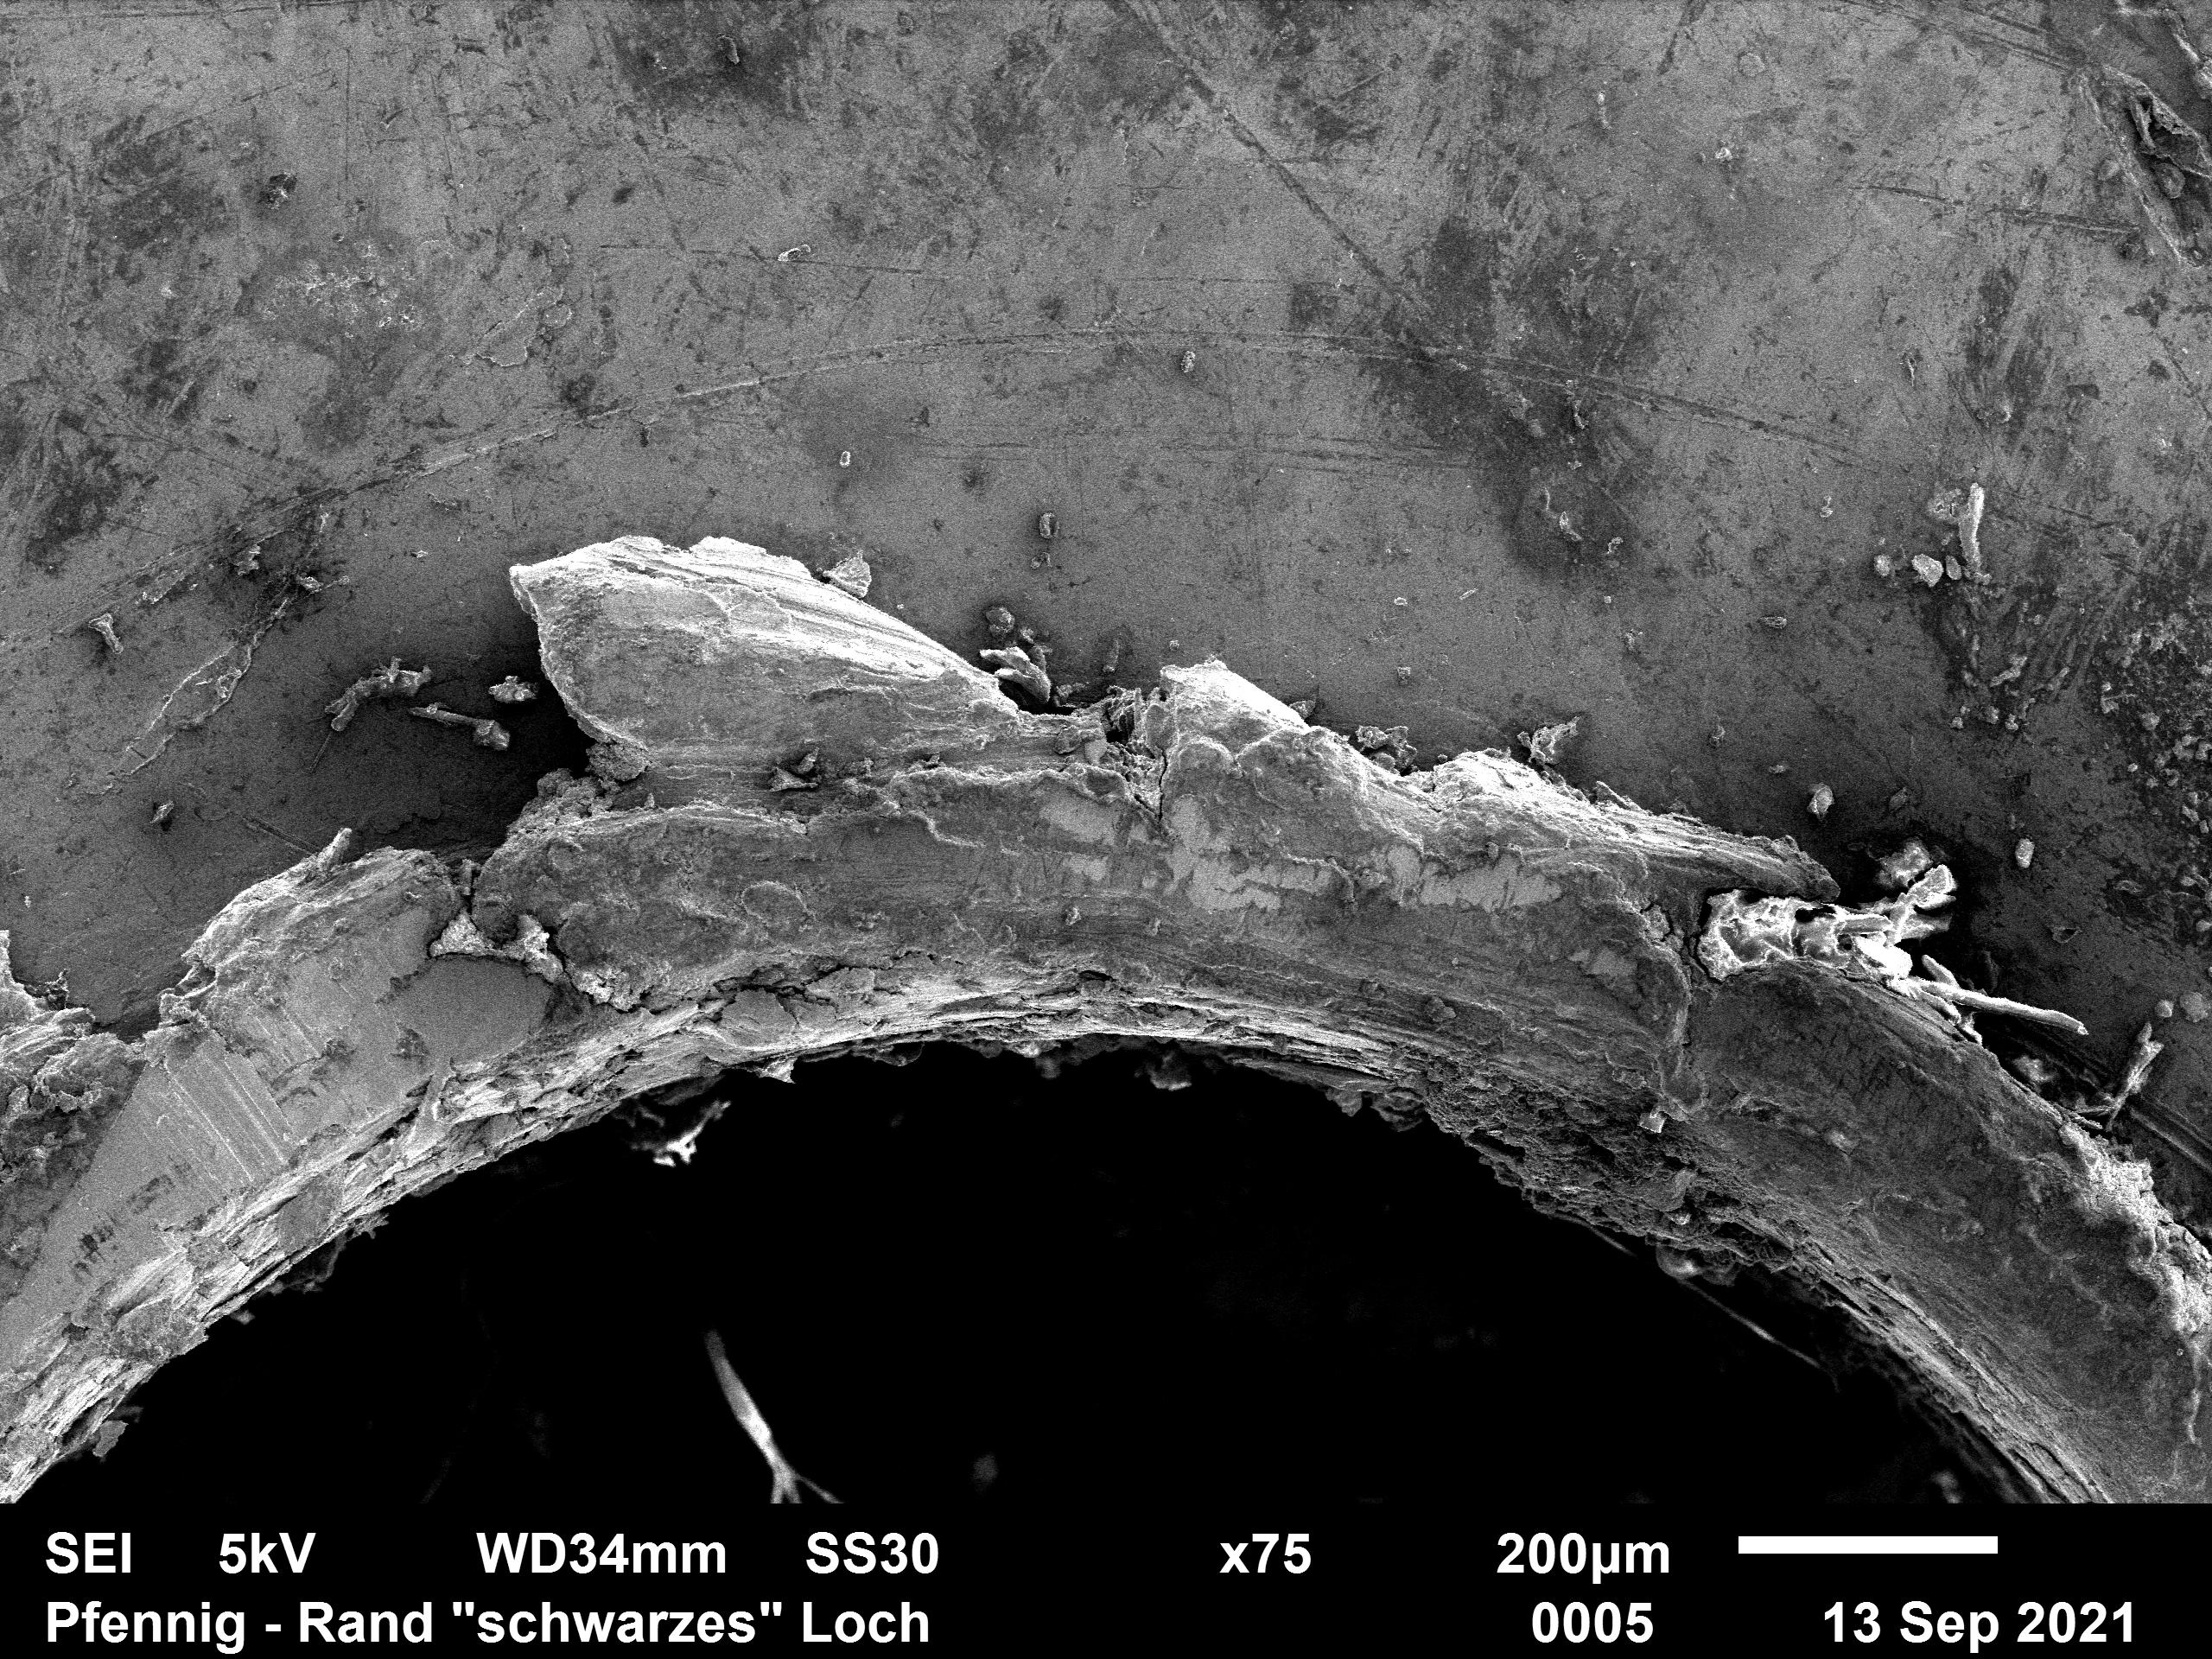
\includegraphics[width=\textwidth]{Auswertung/A/0005.png}
        \caption{$U_B = 5$ kV}
    \end{subfigure}
    \hfill
    \begin{subfigure}[b]{0.45\textwidth}
        \centering
        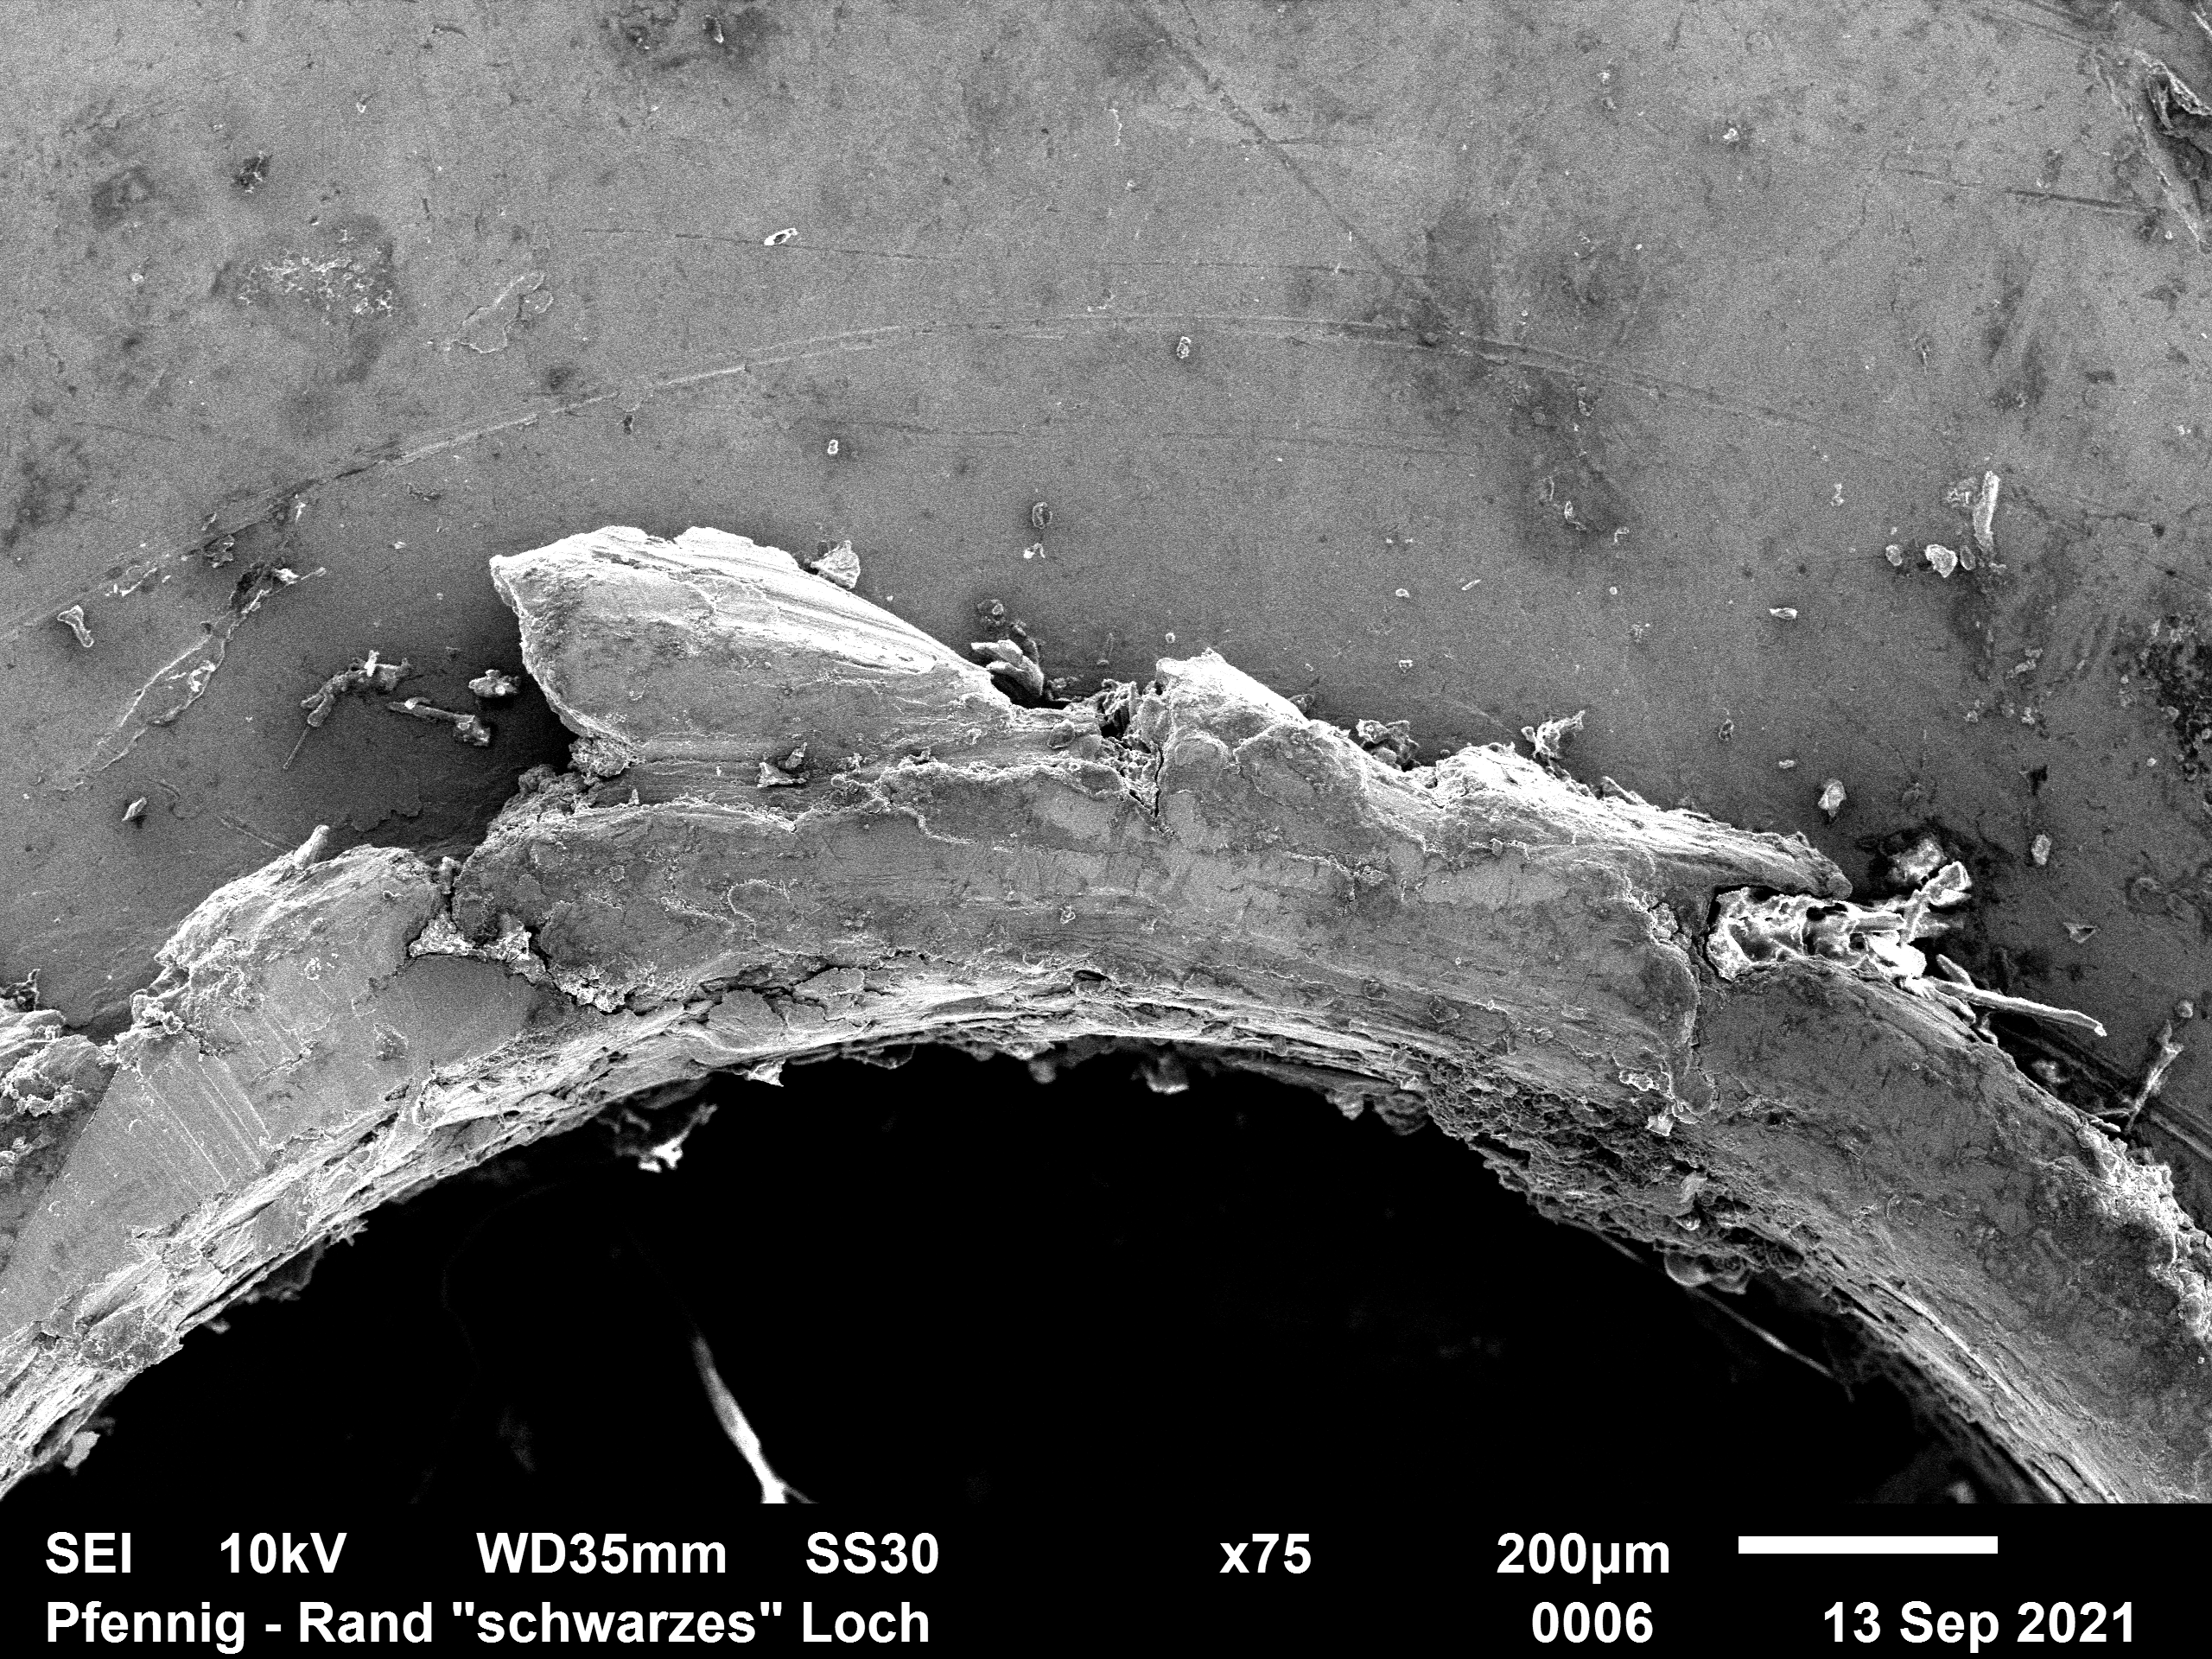
\includegraphics[width=\textwidth]{Auswertung/A/0006.png}
        \caption{$U_B = 10$ kV}
    \end{subfigure}
    \\
    \begin{subfigure}[b]{0.45\textwidth}
        \centering
        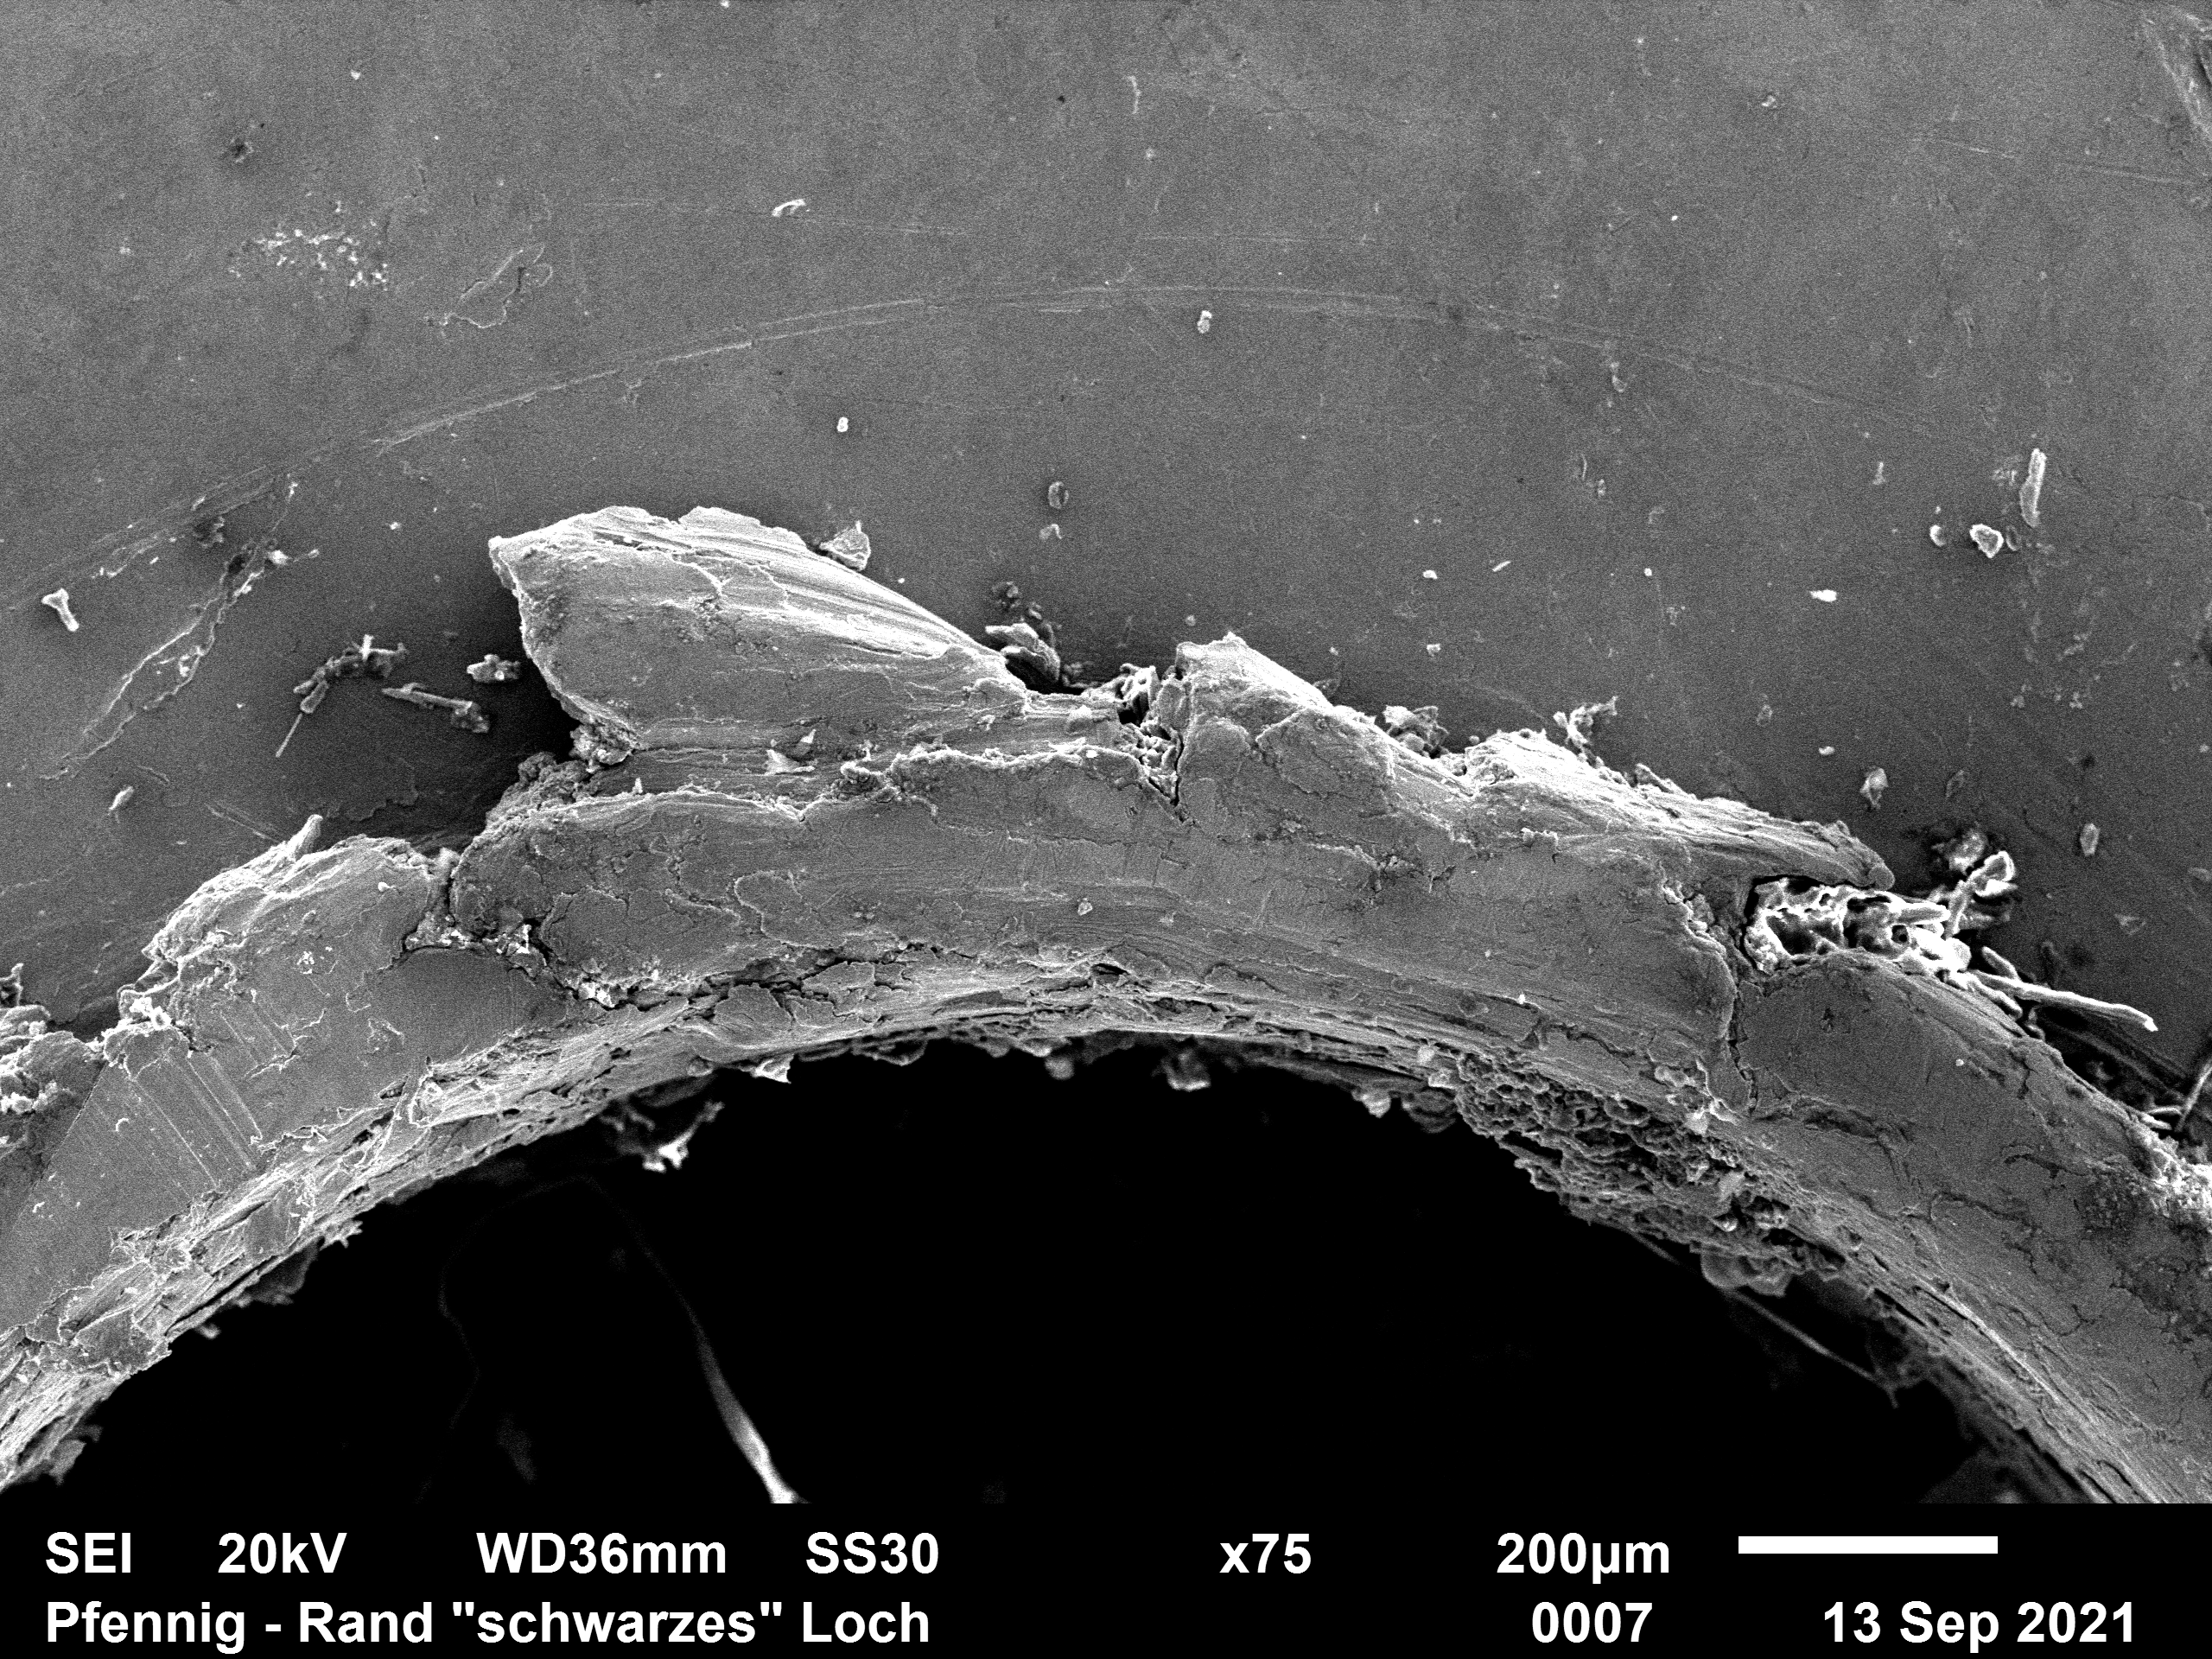
\includegraphics[width=\textwidth]{Auswertung/A/0007.png}
        \caption{$U_B = 20$ kV}
    \end{subfigure}
    \hfill
    \begin{subfigure}[b]{0.45\textwidth}
        \centering
        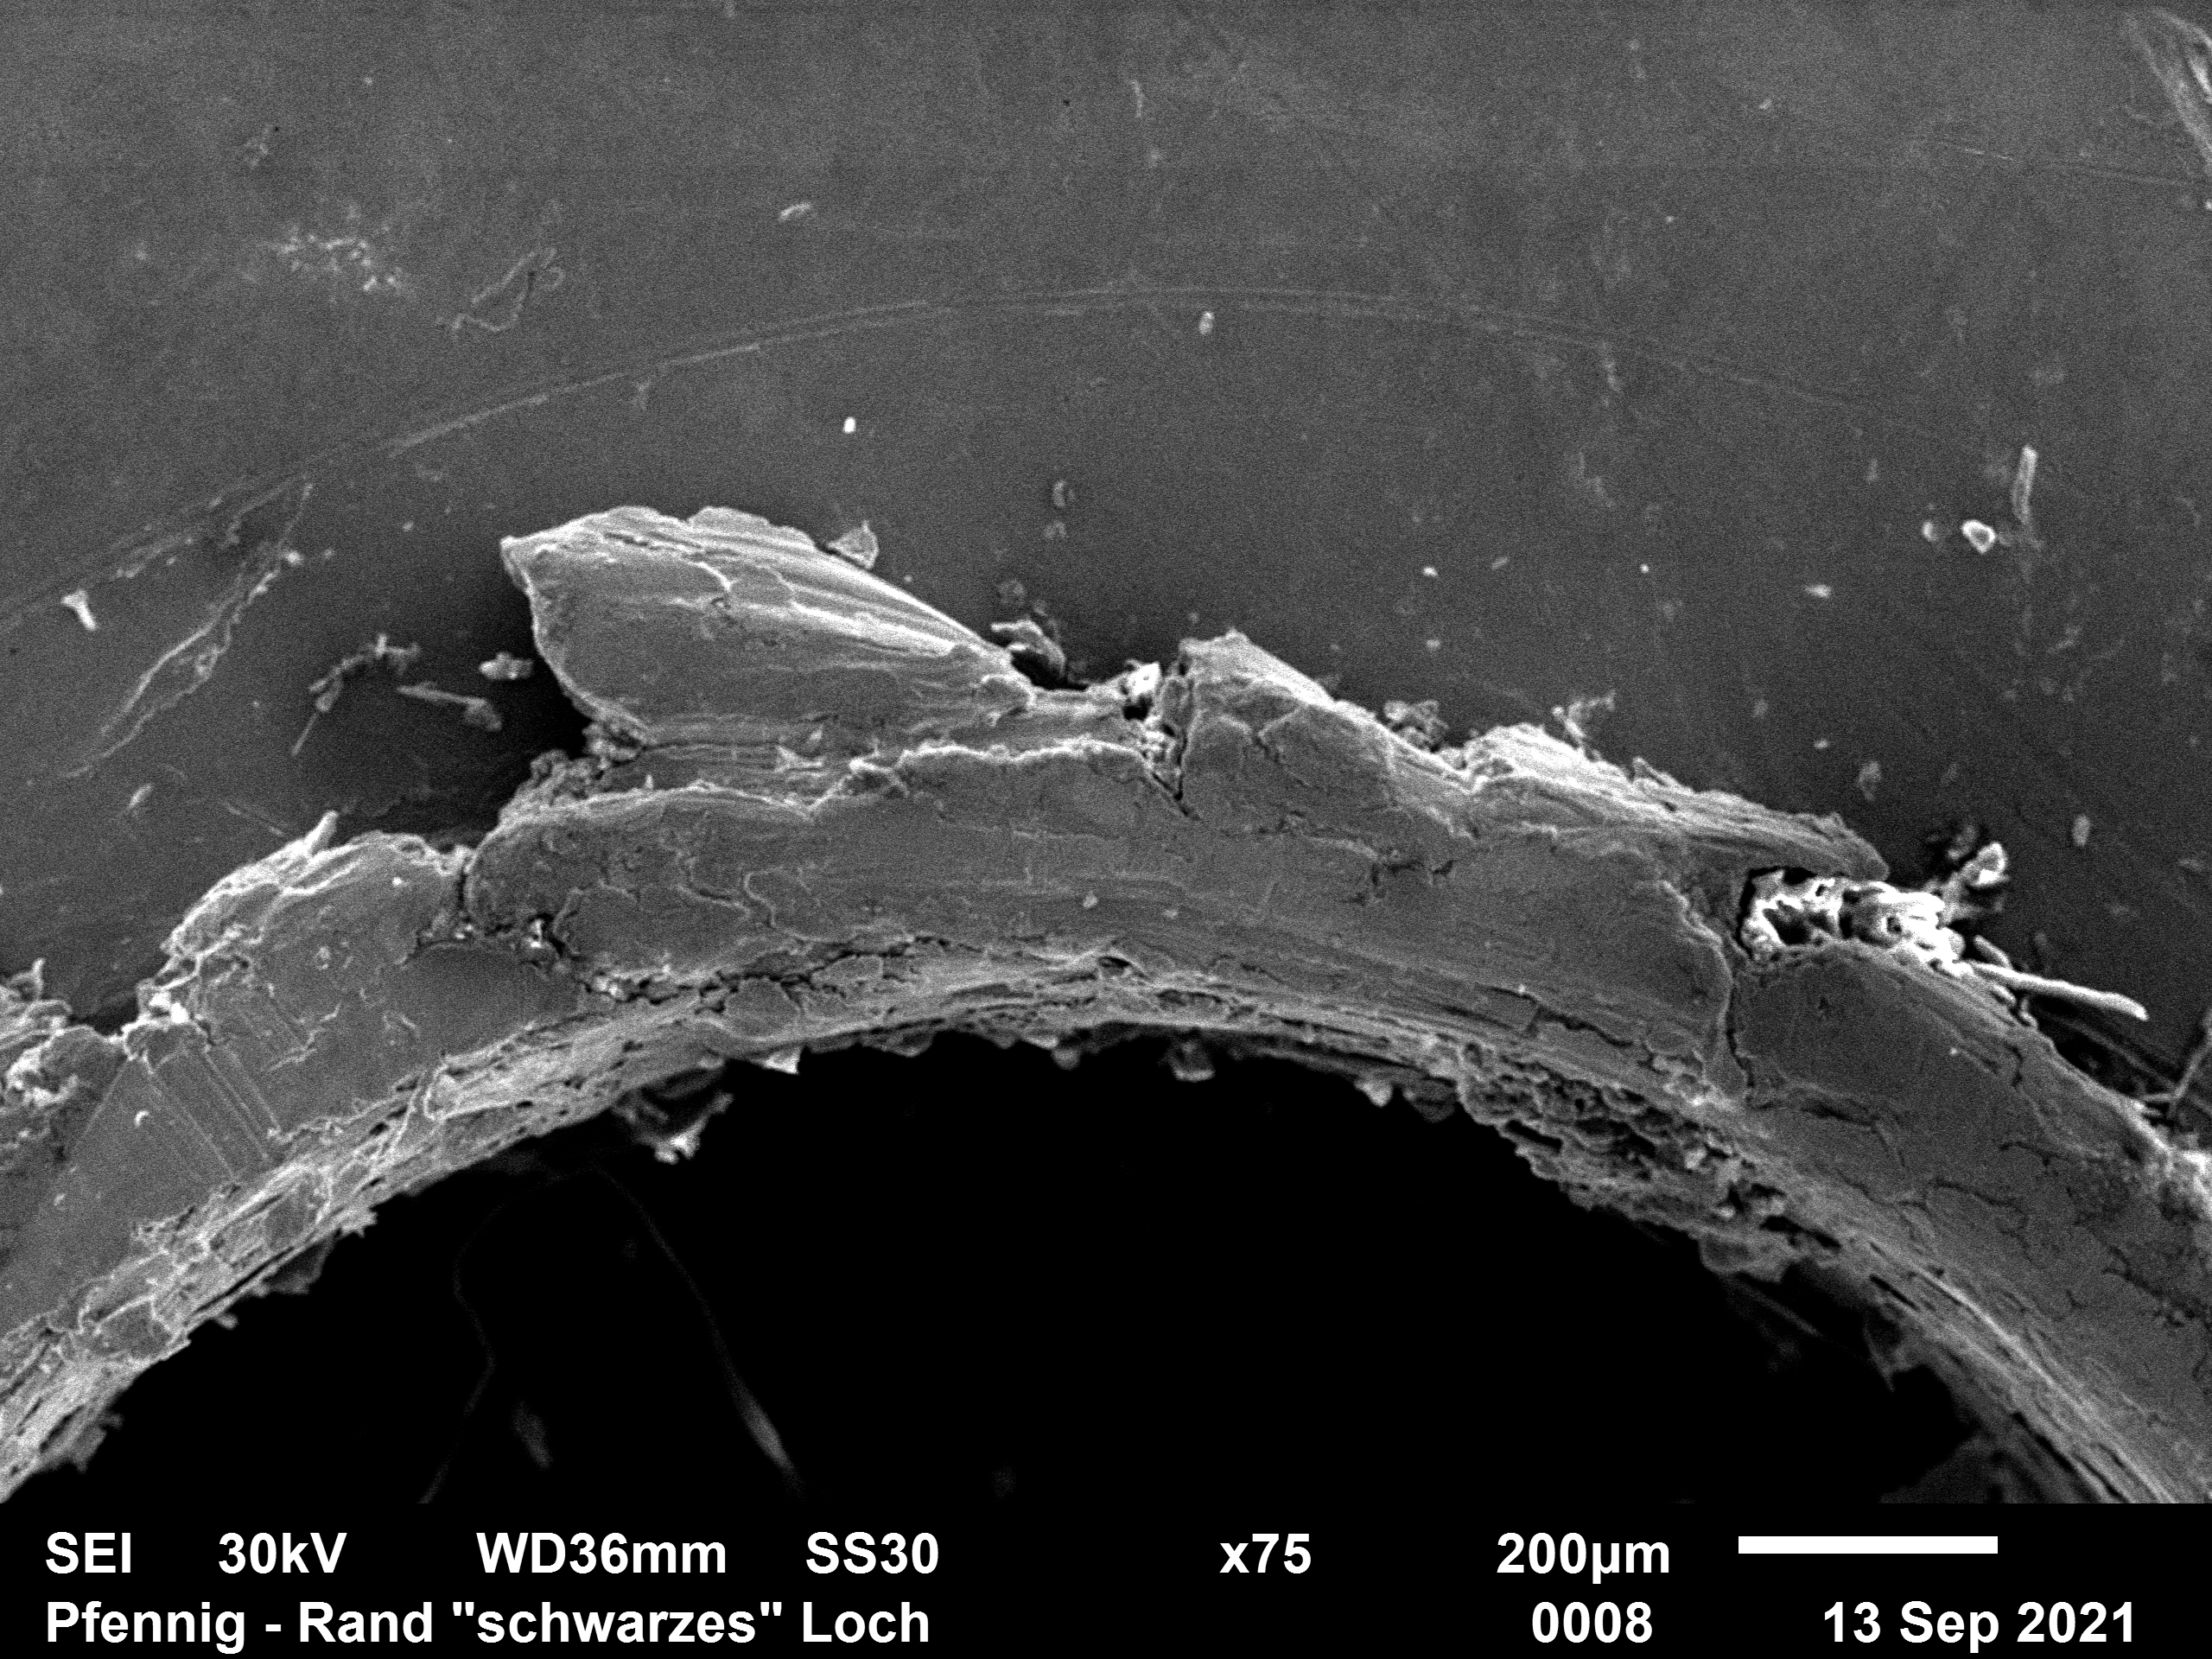
\includegraphics[width=\textwidth]{Auswertung/A/0008.png}
        \caption{$U_B = 30$ kV}
    \end{subfigure}
    \caption{SEI bei unterschiedlichen Beschleunigunsspannungen}
\end{figure}

Für niedrige Spannungen sind zunehmend Flecken auf der glatten Fläche zu erkennen, was möglicherweise durch Verunreinigungen auf der Probenoberfläche verursacht wird, welch bei niedrigerer Energie der Elektronen mehr ins Gewicht fallen. Elektronen mit niedriger Energie werden durch diese Rückstände weiter entschleunigt, weshalb dann dunkle Flecken zu erkennen sind.

\newpage
Als Nächstes wurde der Everhart-Thronley-Detektor im RE Modus (REF) verwendet und dabei ebenfalls die Beschleunigungsspannung variiert.
\begin{figure}[h]
    \centering
    
    \begin{subfigure}[b]{0.45\textwidth}
        \centering
        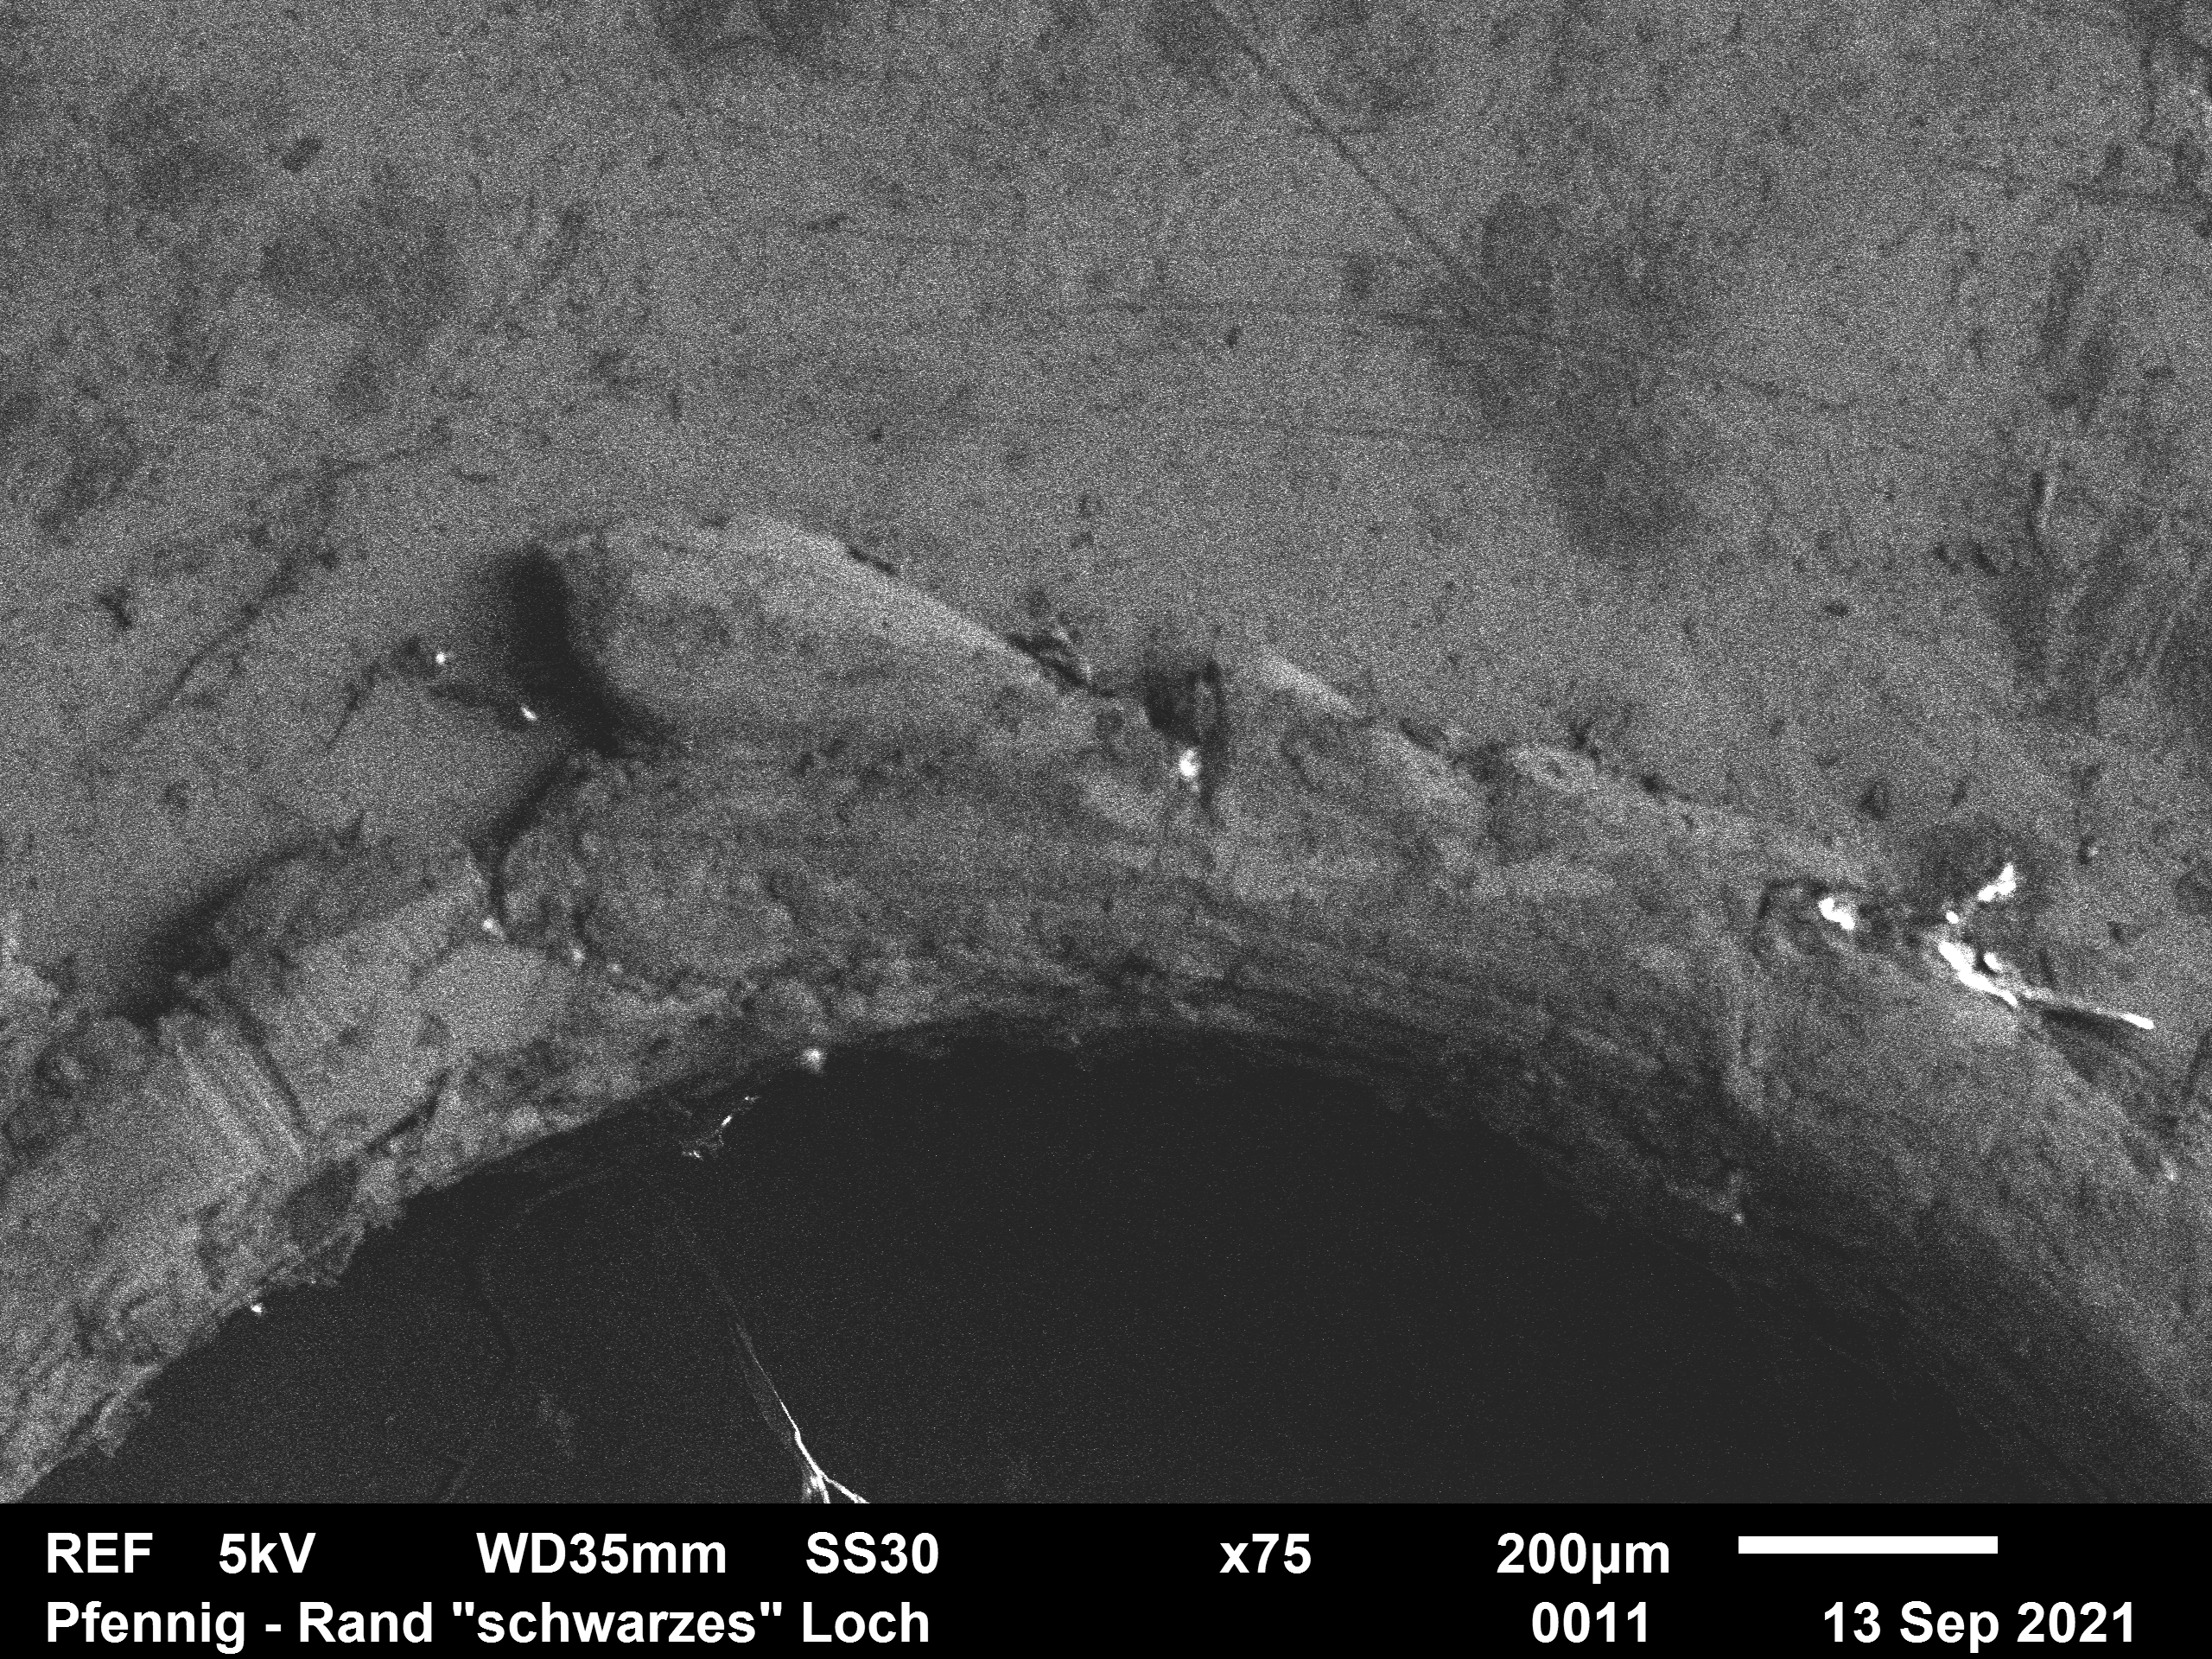
\includegraphics[width=\textwidth]{Auswertung/A/0011.png}
        \caption{$U_B = 5$ kV}
    \end{subfigure}
    \hfill
    \begin{subfigure}[b]{0.45\textwidth}
        \centering
        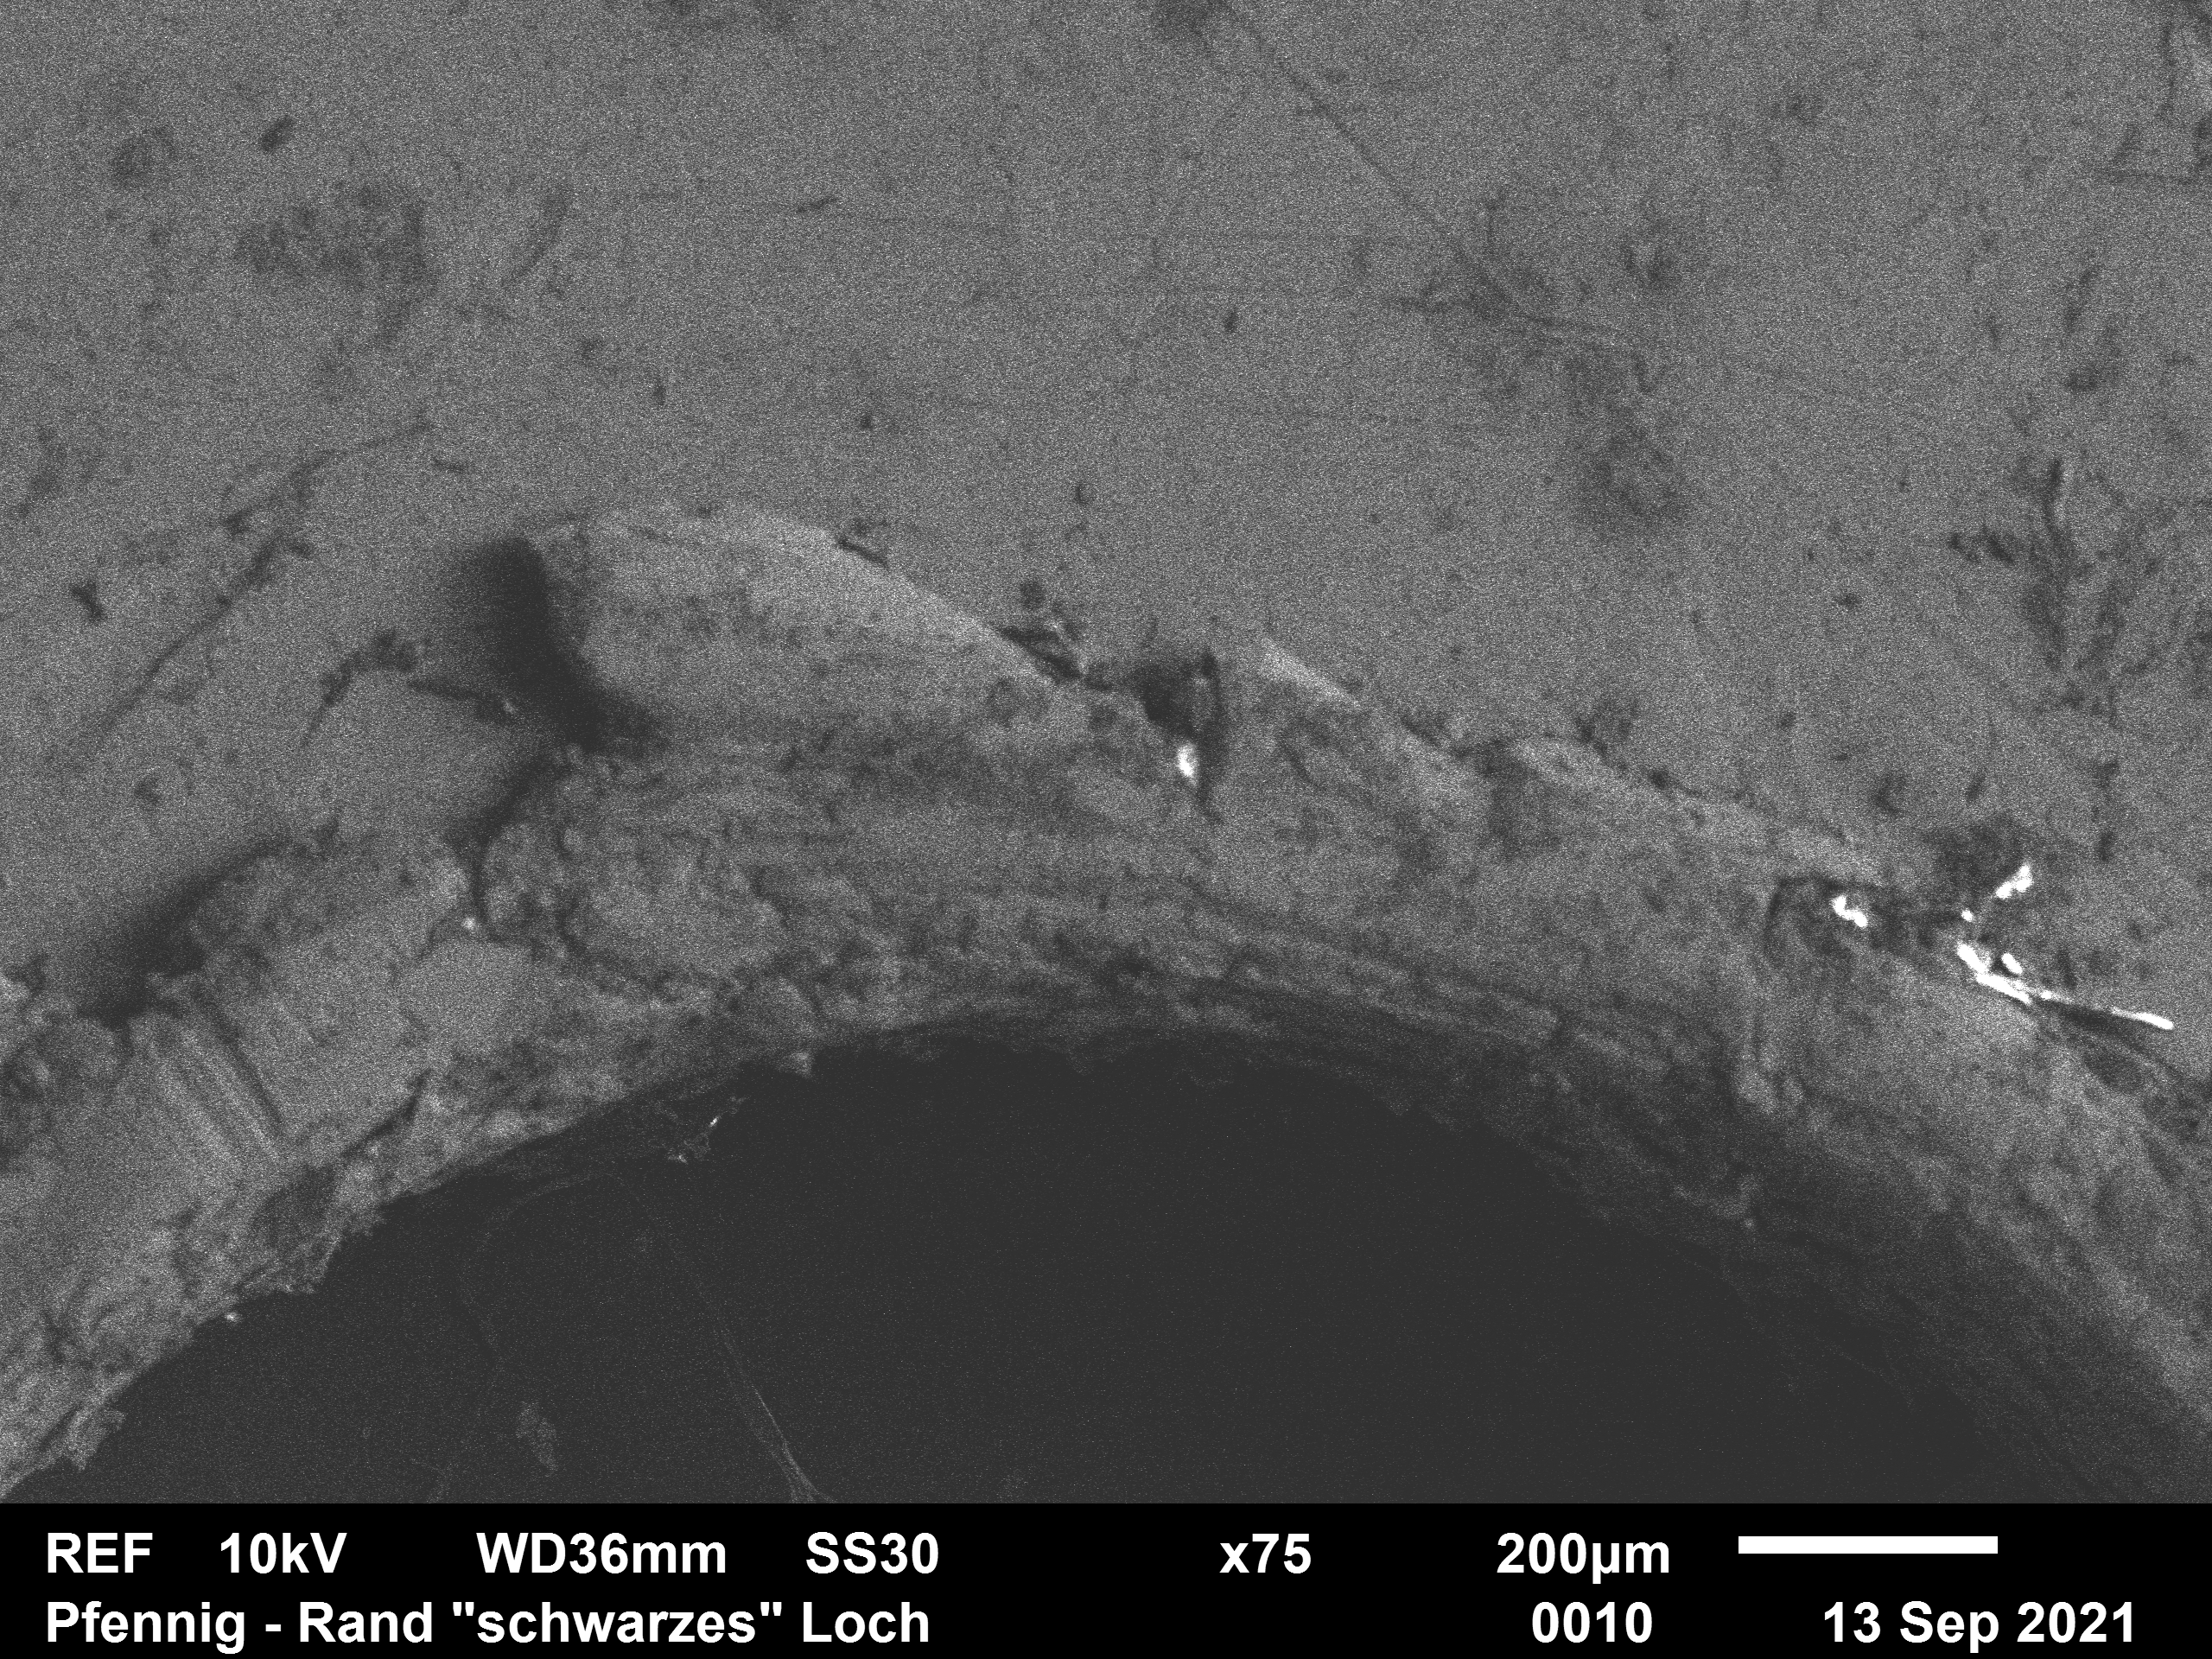
\includegraphics[width=\textwidth]{Auswertung/A/0010.png}
        \caption{$U_B = 10$ kV}
    \end{subfigure}
    \\
    \begin{subfigure}[b]{0.45\textwidth}
        \centering
        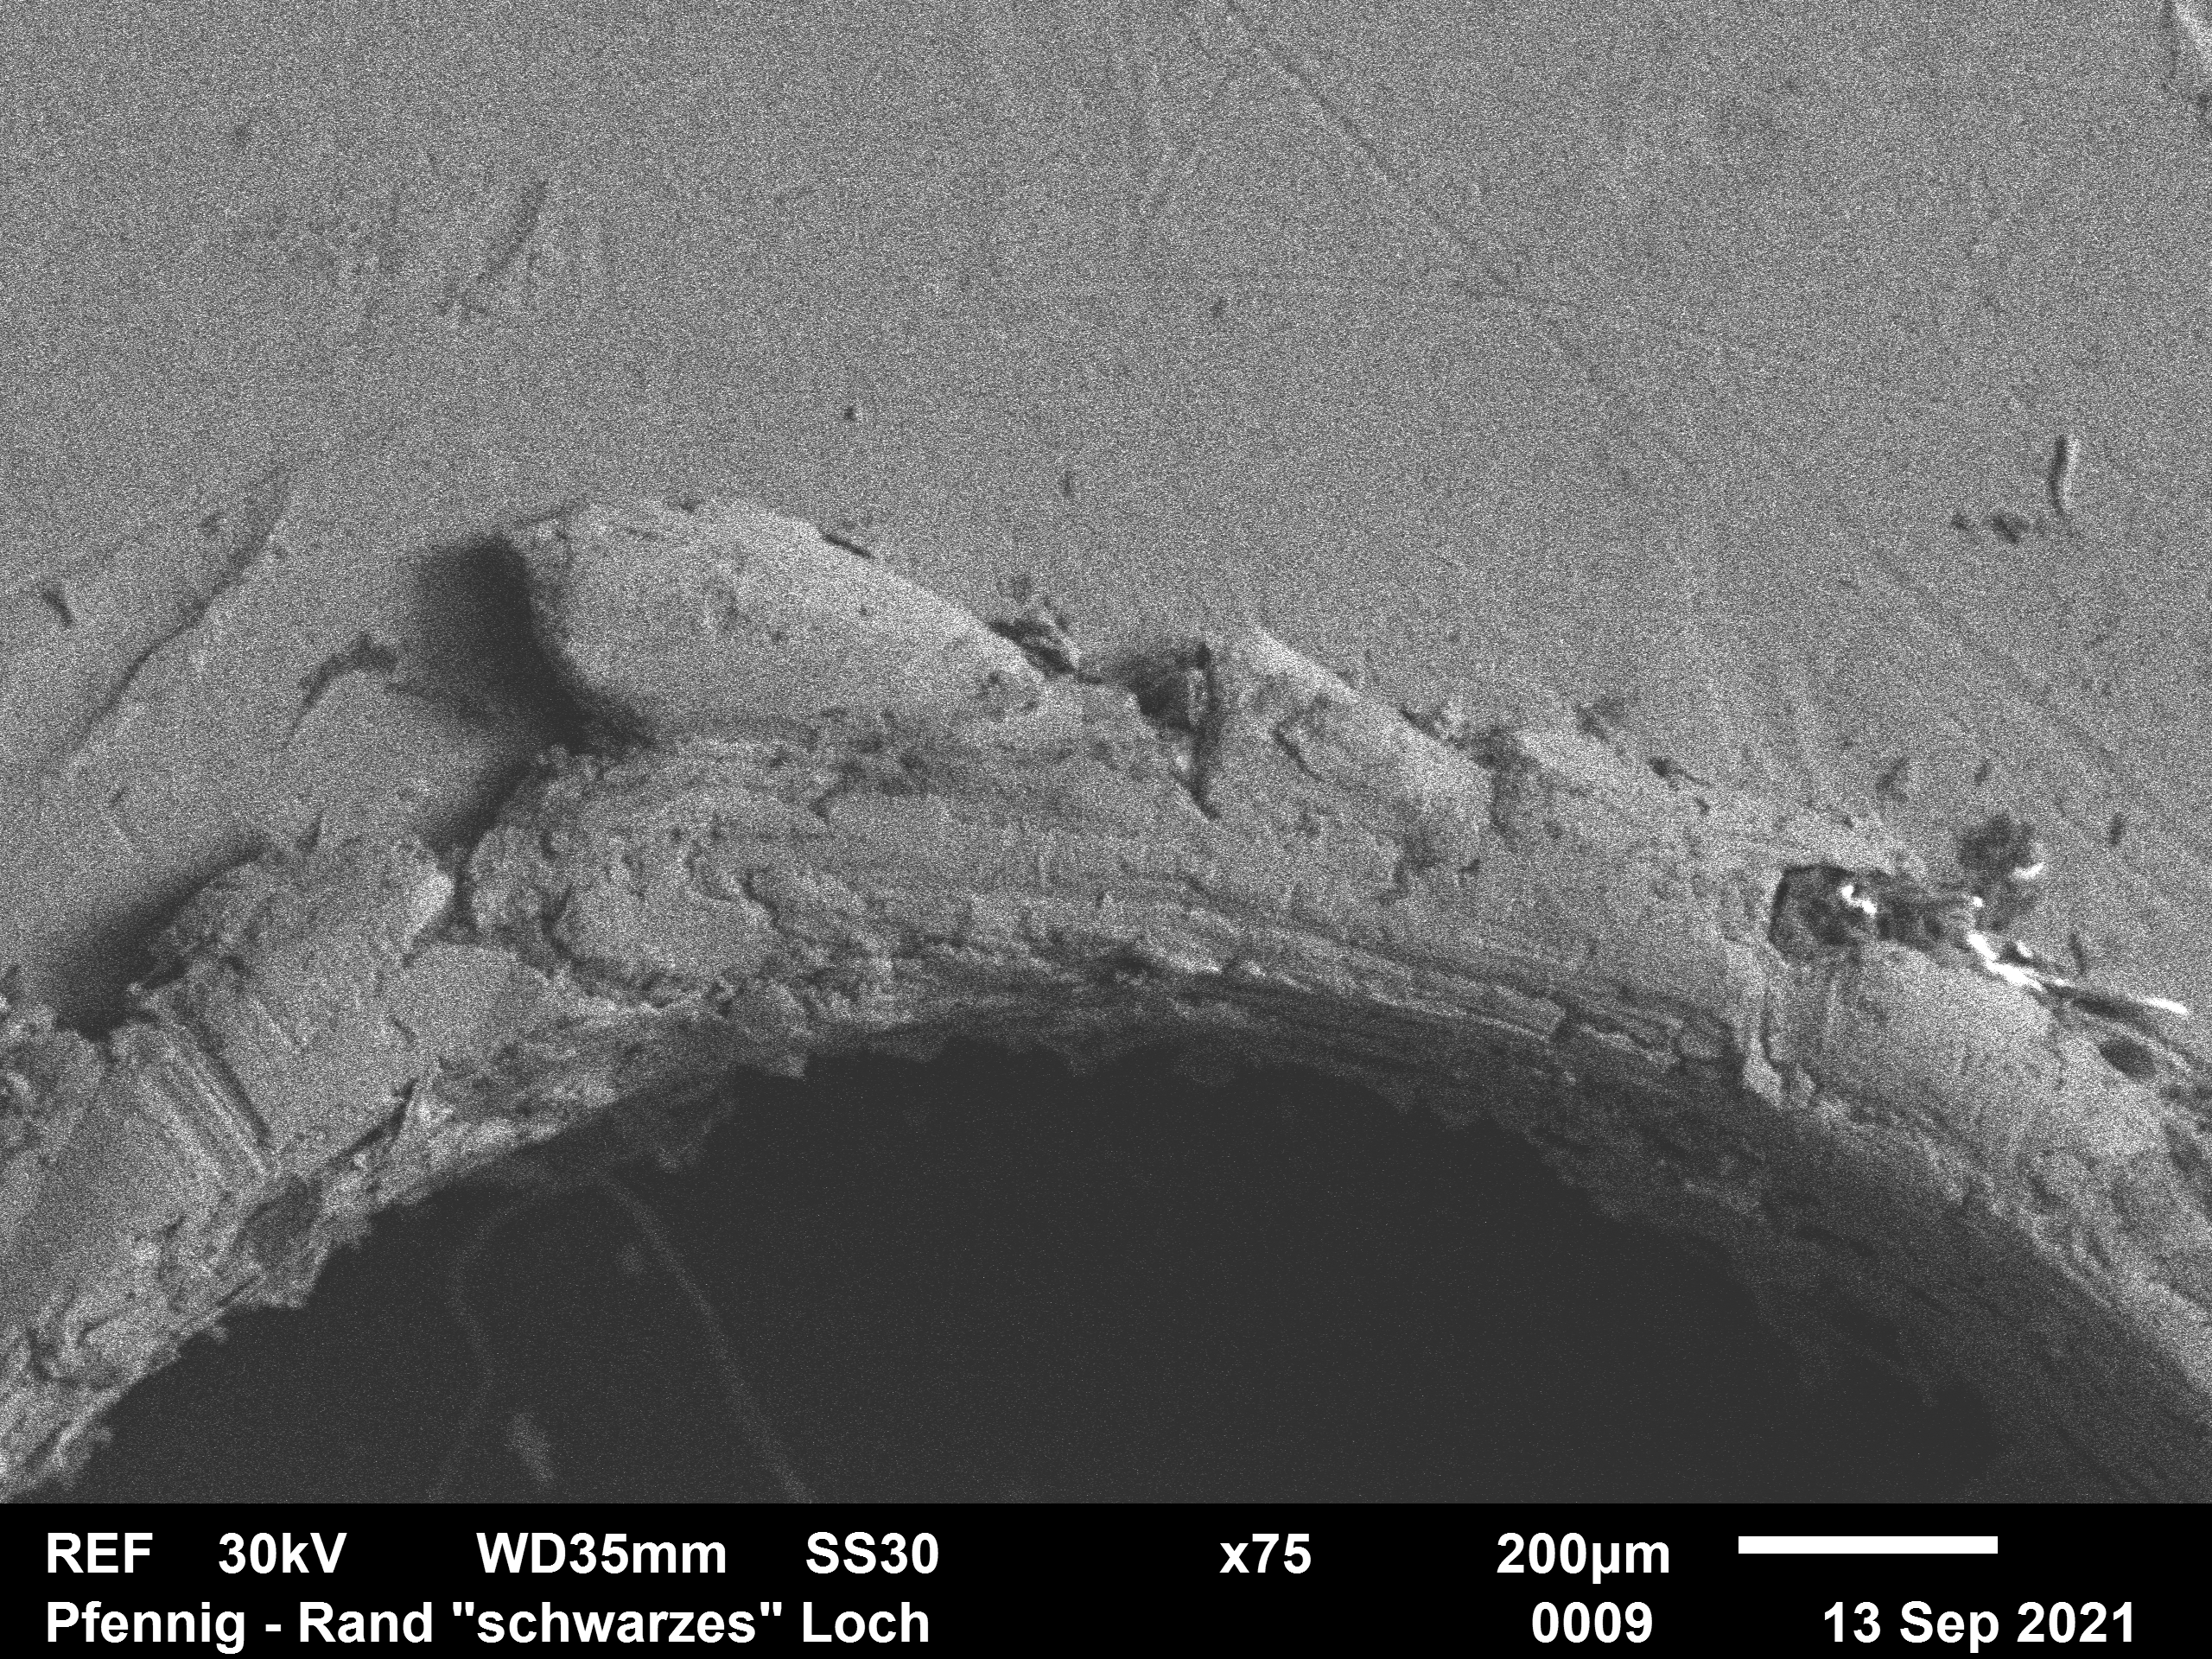
\includegraphics[width=\textwidth]{Auswertung/A/0009.png}
        \caption{$U_B = 30$ kV}
    \end{subfigure}
    \caption{REF bei unterschiedlichen Beschleunigunsspannungen}
\end{figure}

Genau wie oben sind bei niedriger Energie der Primärelektronen dunkle Flecken zu erkennen.\\
Weiterhin sind Abschattungskontraste der Bereiche, welche im Schatten des Everhart-Thronley-Detektors liegen, gut zu erkennen.

\newpage
Das gleich wurde auch für den Halbleiterdetektor im Compo-Mode (BEC) gemacht.
\begin{figure}[h]
    \centering
    
    \begin{subfigure}[b]{0.45\textwidth}
        \centering
        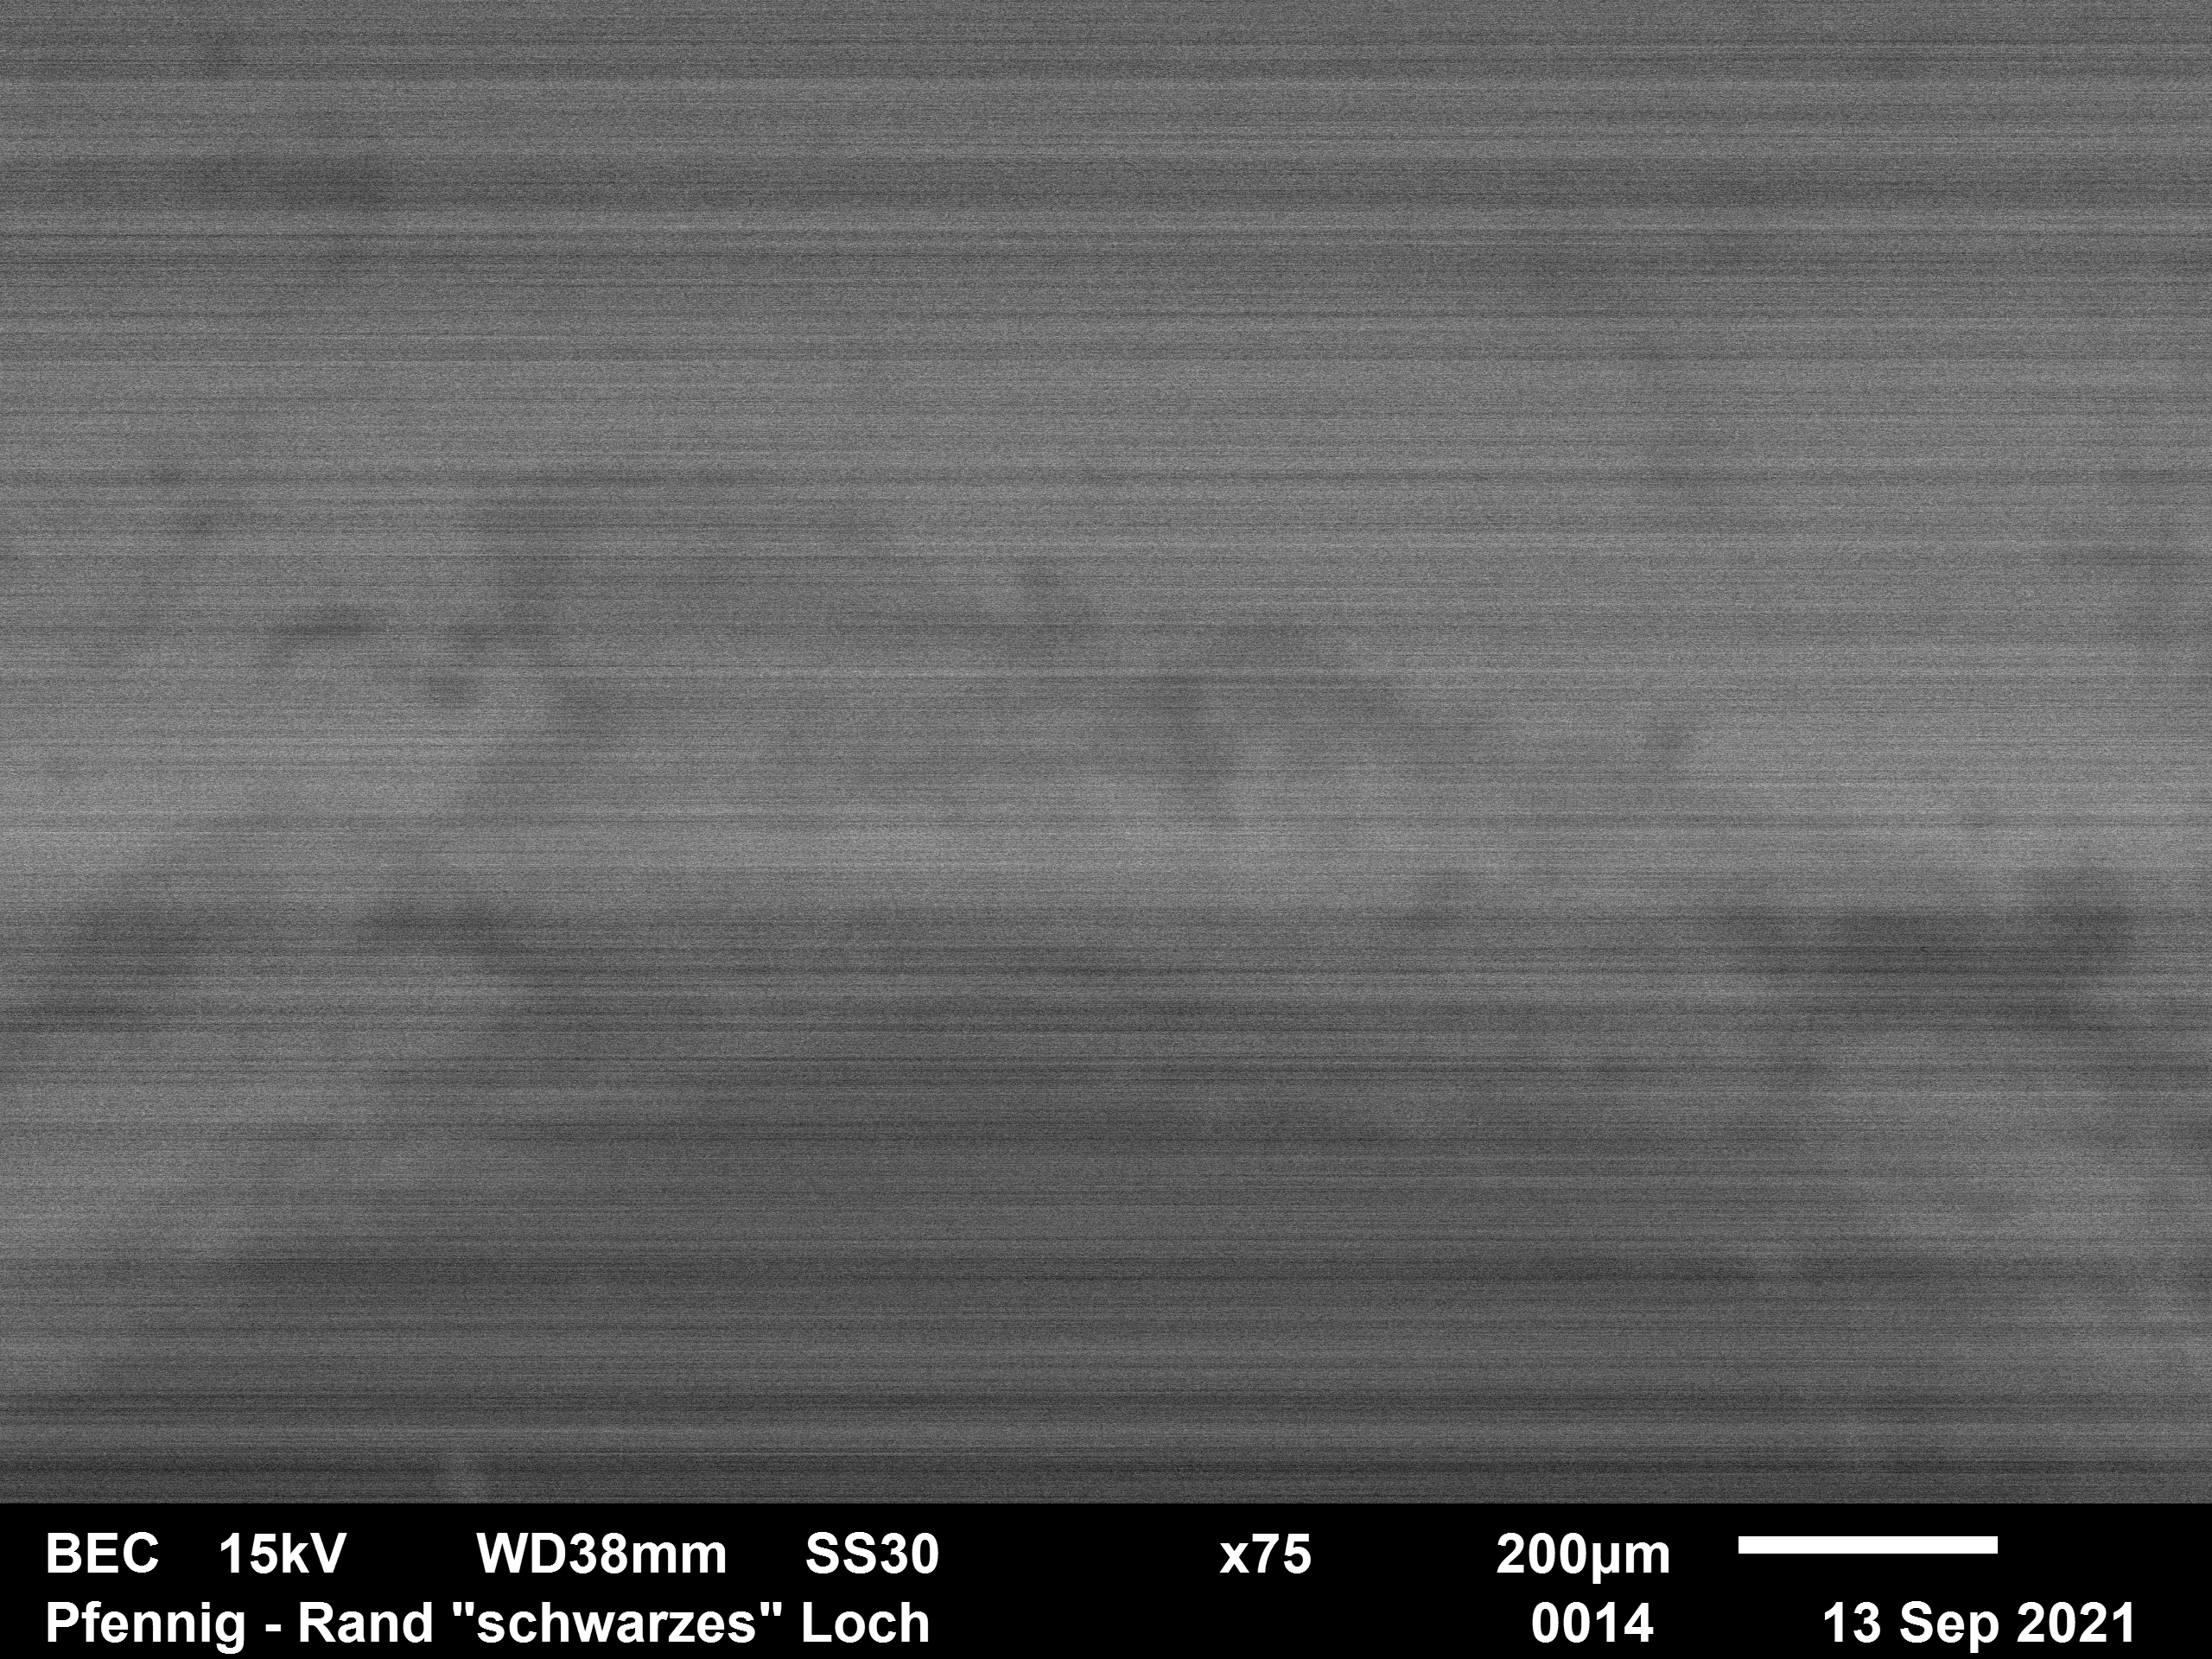
\includegraphics[width=\textwidth]{Auswertung/A/0014.png}
        \caption{$U_B = 15$ kV}
    \end{subfigure}
    \hfill
    \begin{subfigure}[b]{0.45\textwidth}
        \centering
        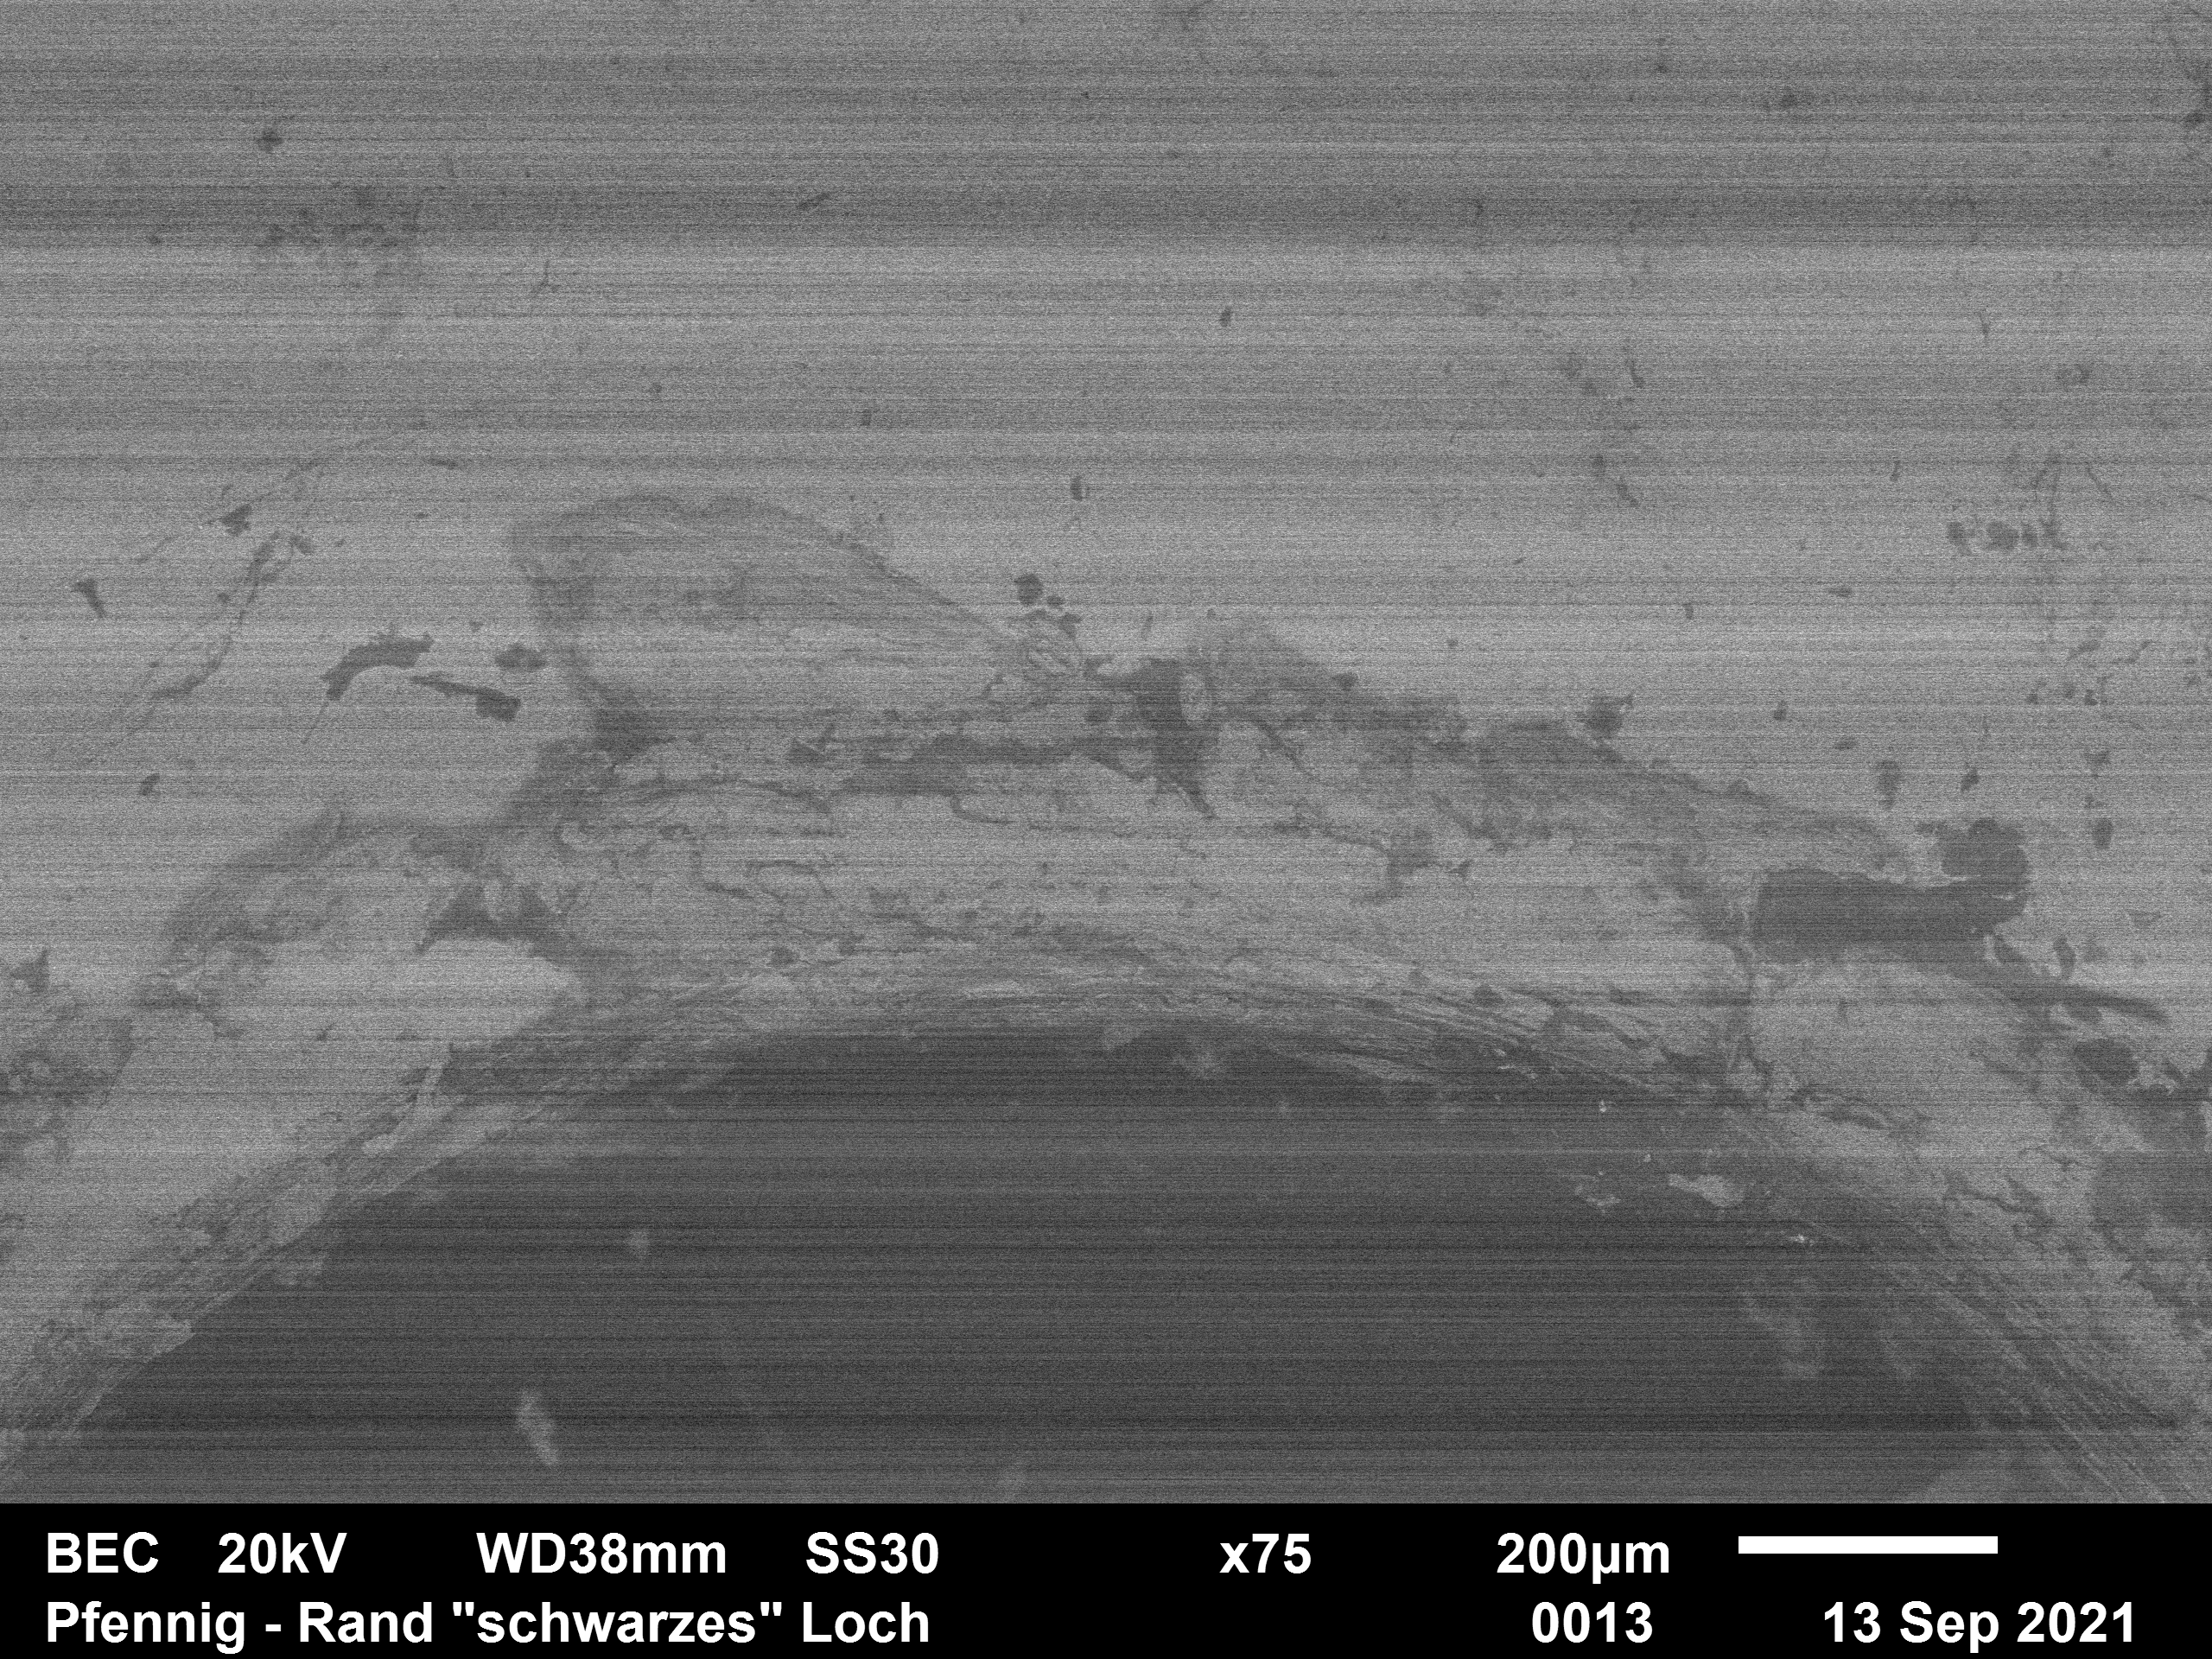
\includegraphics[width=\textwidth]{Auswertung/A/0013.png}
        \caption{$U_B = 20$ kV}
    \end{subfigure}
    \\
    \begin{subfigure}[b]{0.45\textwidth}
        \centering
        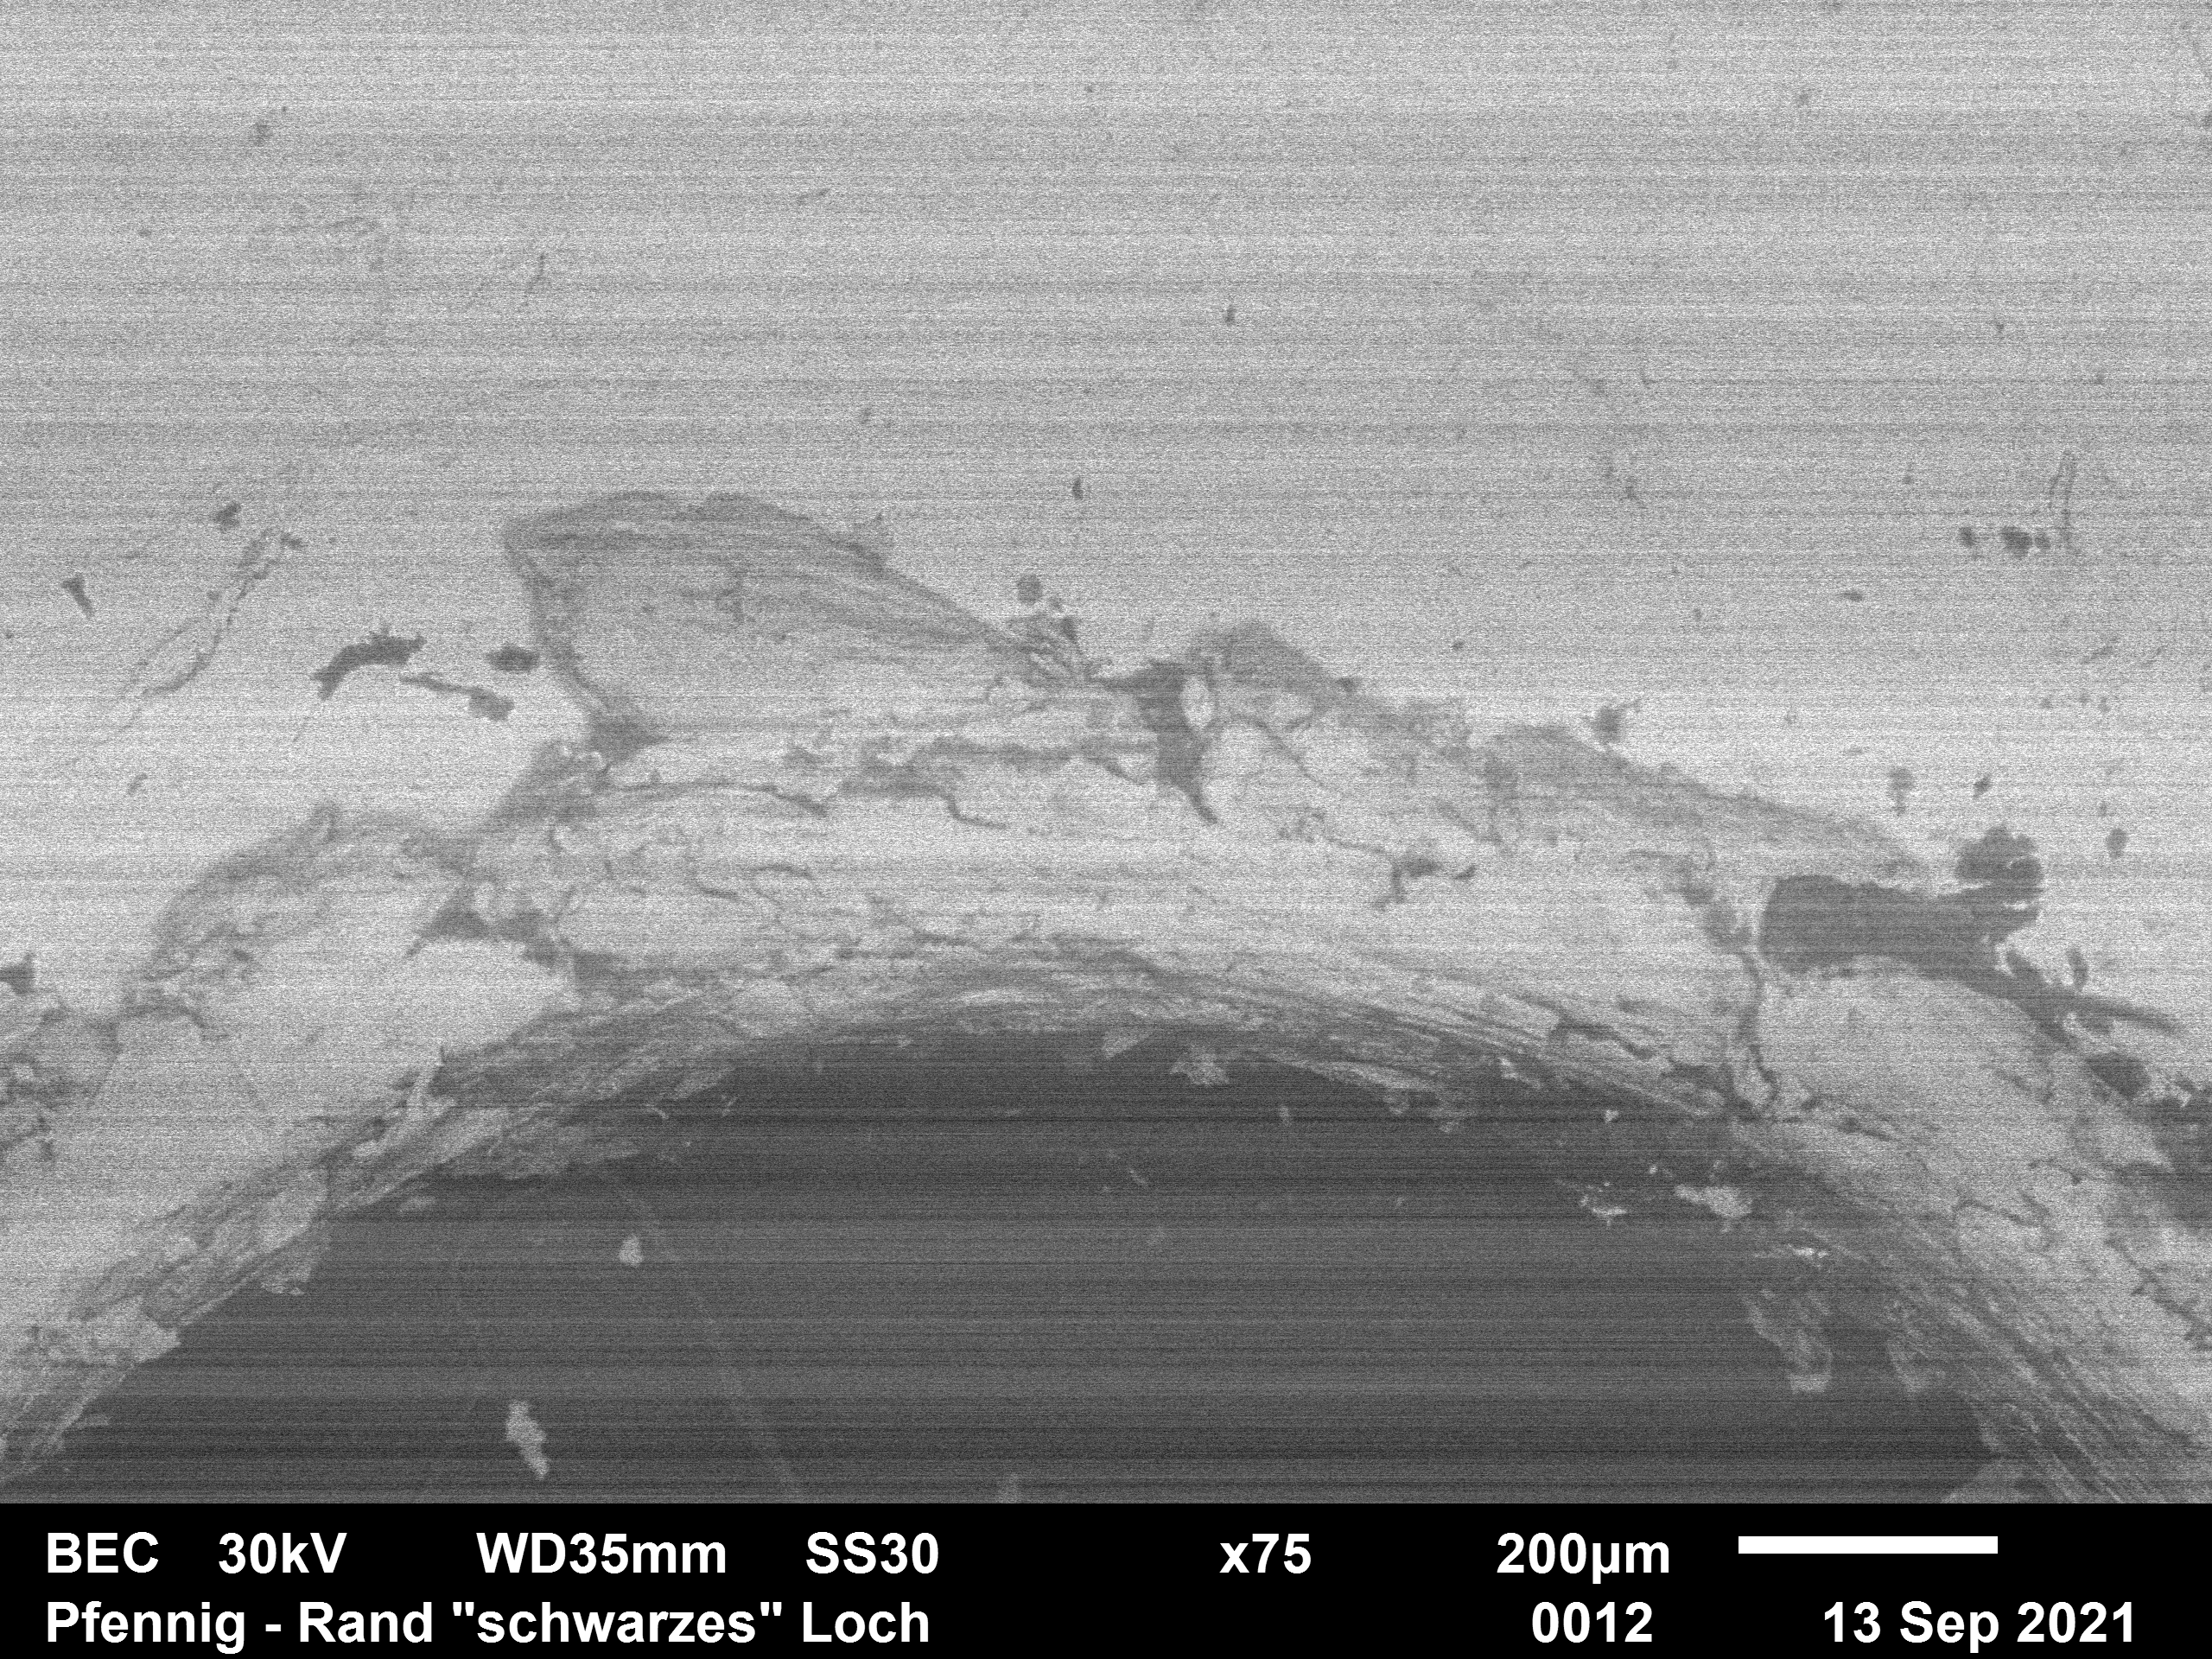
\includegraphics[width=\textwidth]{Auswertung/A/0012.png}
        \caption{$U_B = 30$ kV}
    \end{subfigure}
    \caption{BEC bei unterschiedlichen Beschleunigunsspannungen}
\end{figure}

Hier fällt sofort auf, dass die Bildqualität rapide mit der Beschleunigungsspannung abfällt. Also muss ein PE Strahl mit niedriger Energie weniger Rückstreuelektronen erzeugen, welche den Halbleiterdetektor erreichen. Dies entspricht auch unseren Erwartungen.

\newpage
Auch für den Halbleiterdetektor im Topo-Mode (BET) wurde die Beschleunigungsspannung variiert.
\begin{figure}[h]
    \centering
    
    \begin{subfigure}[b]{0.45\textwidth}
        \centering
        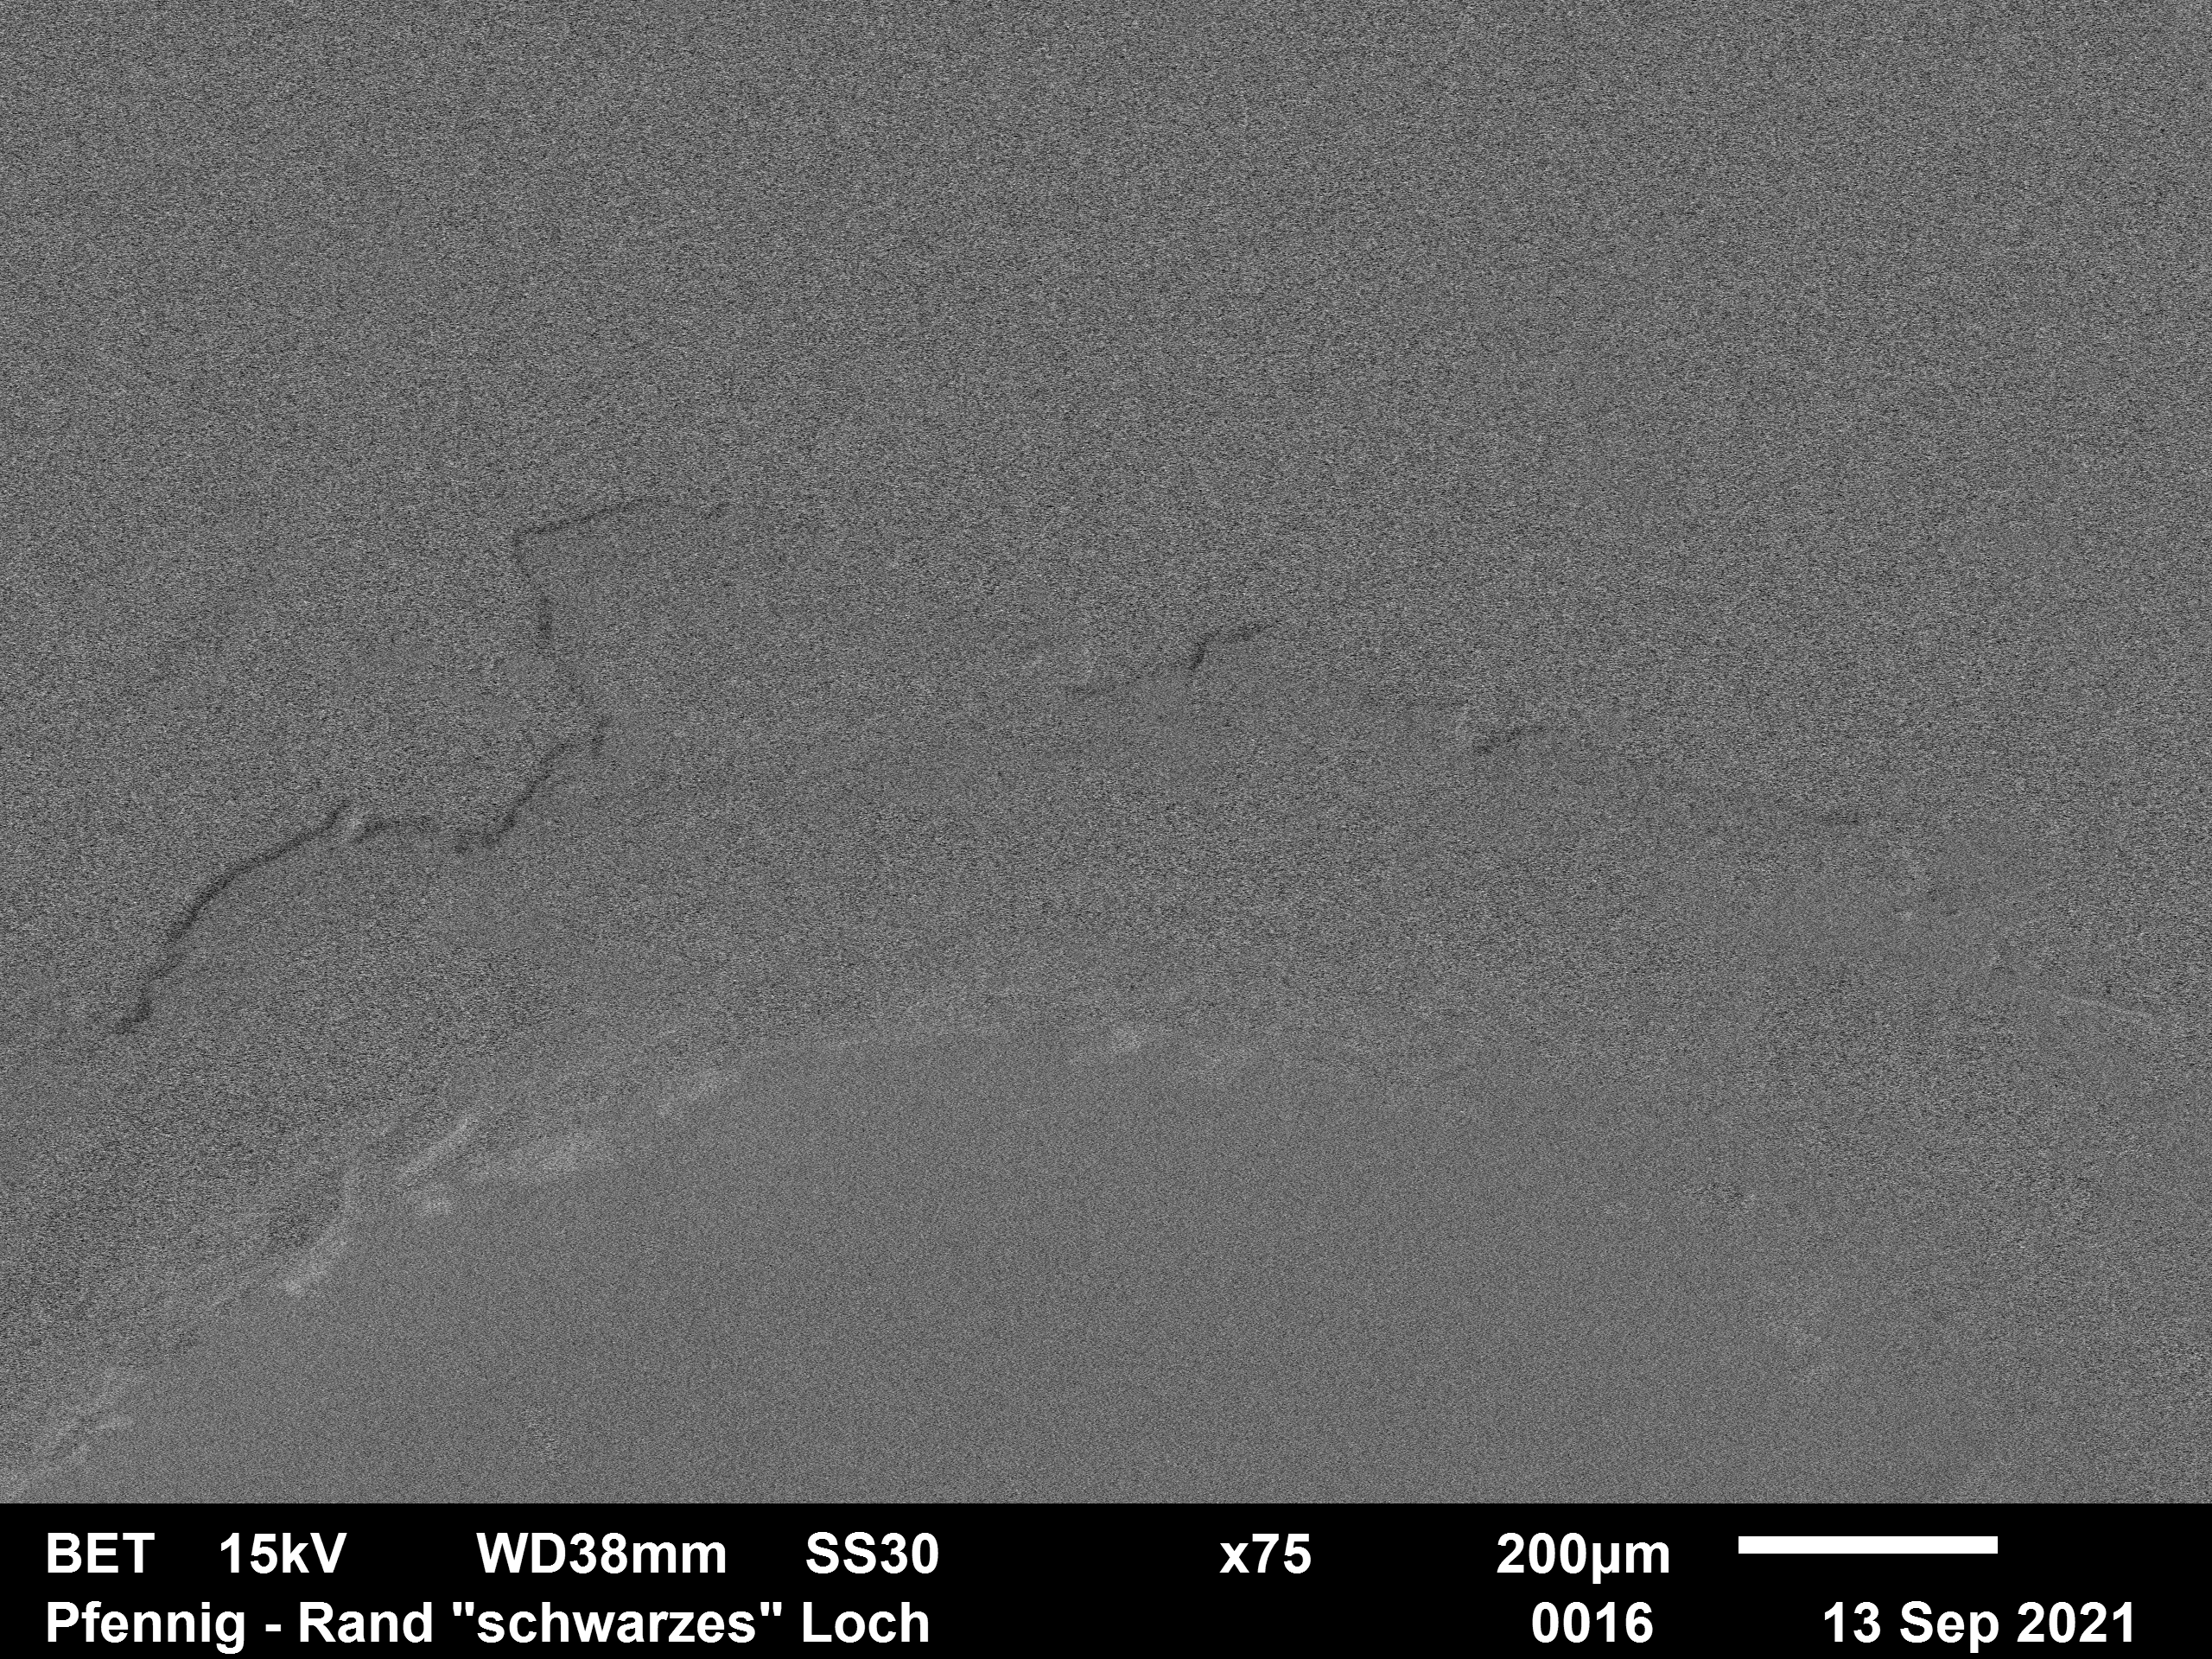
\includegraphics[width=\textwidth]{Auswertung/A/0016.png}
        \caption{$U_B = 15$ kV}
    \end{subfigure}
    \hfill
    \begin{subfigure}[b]{0.45\textwidth}
        \centering
        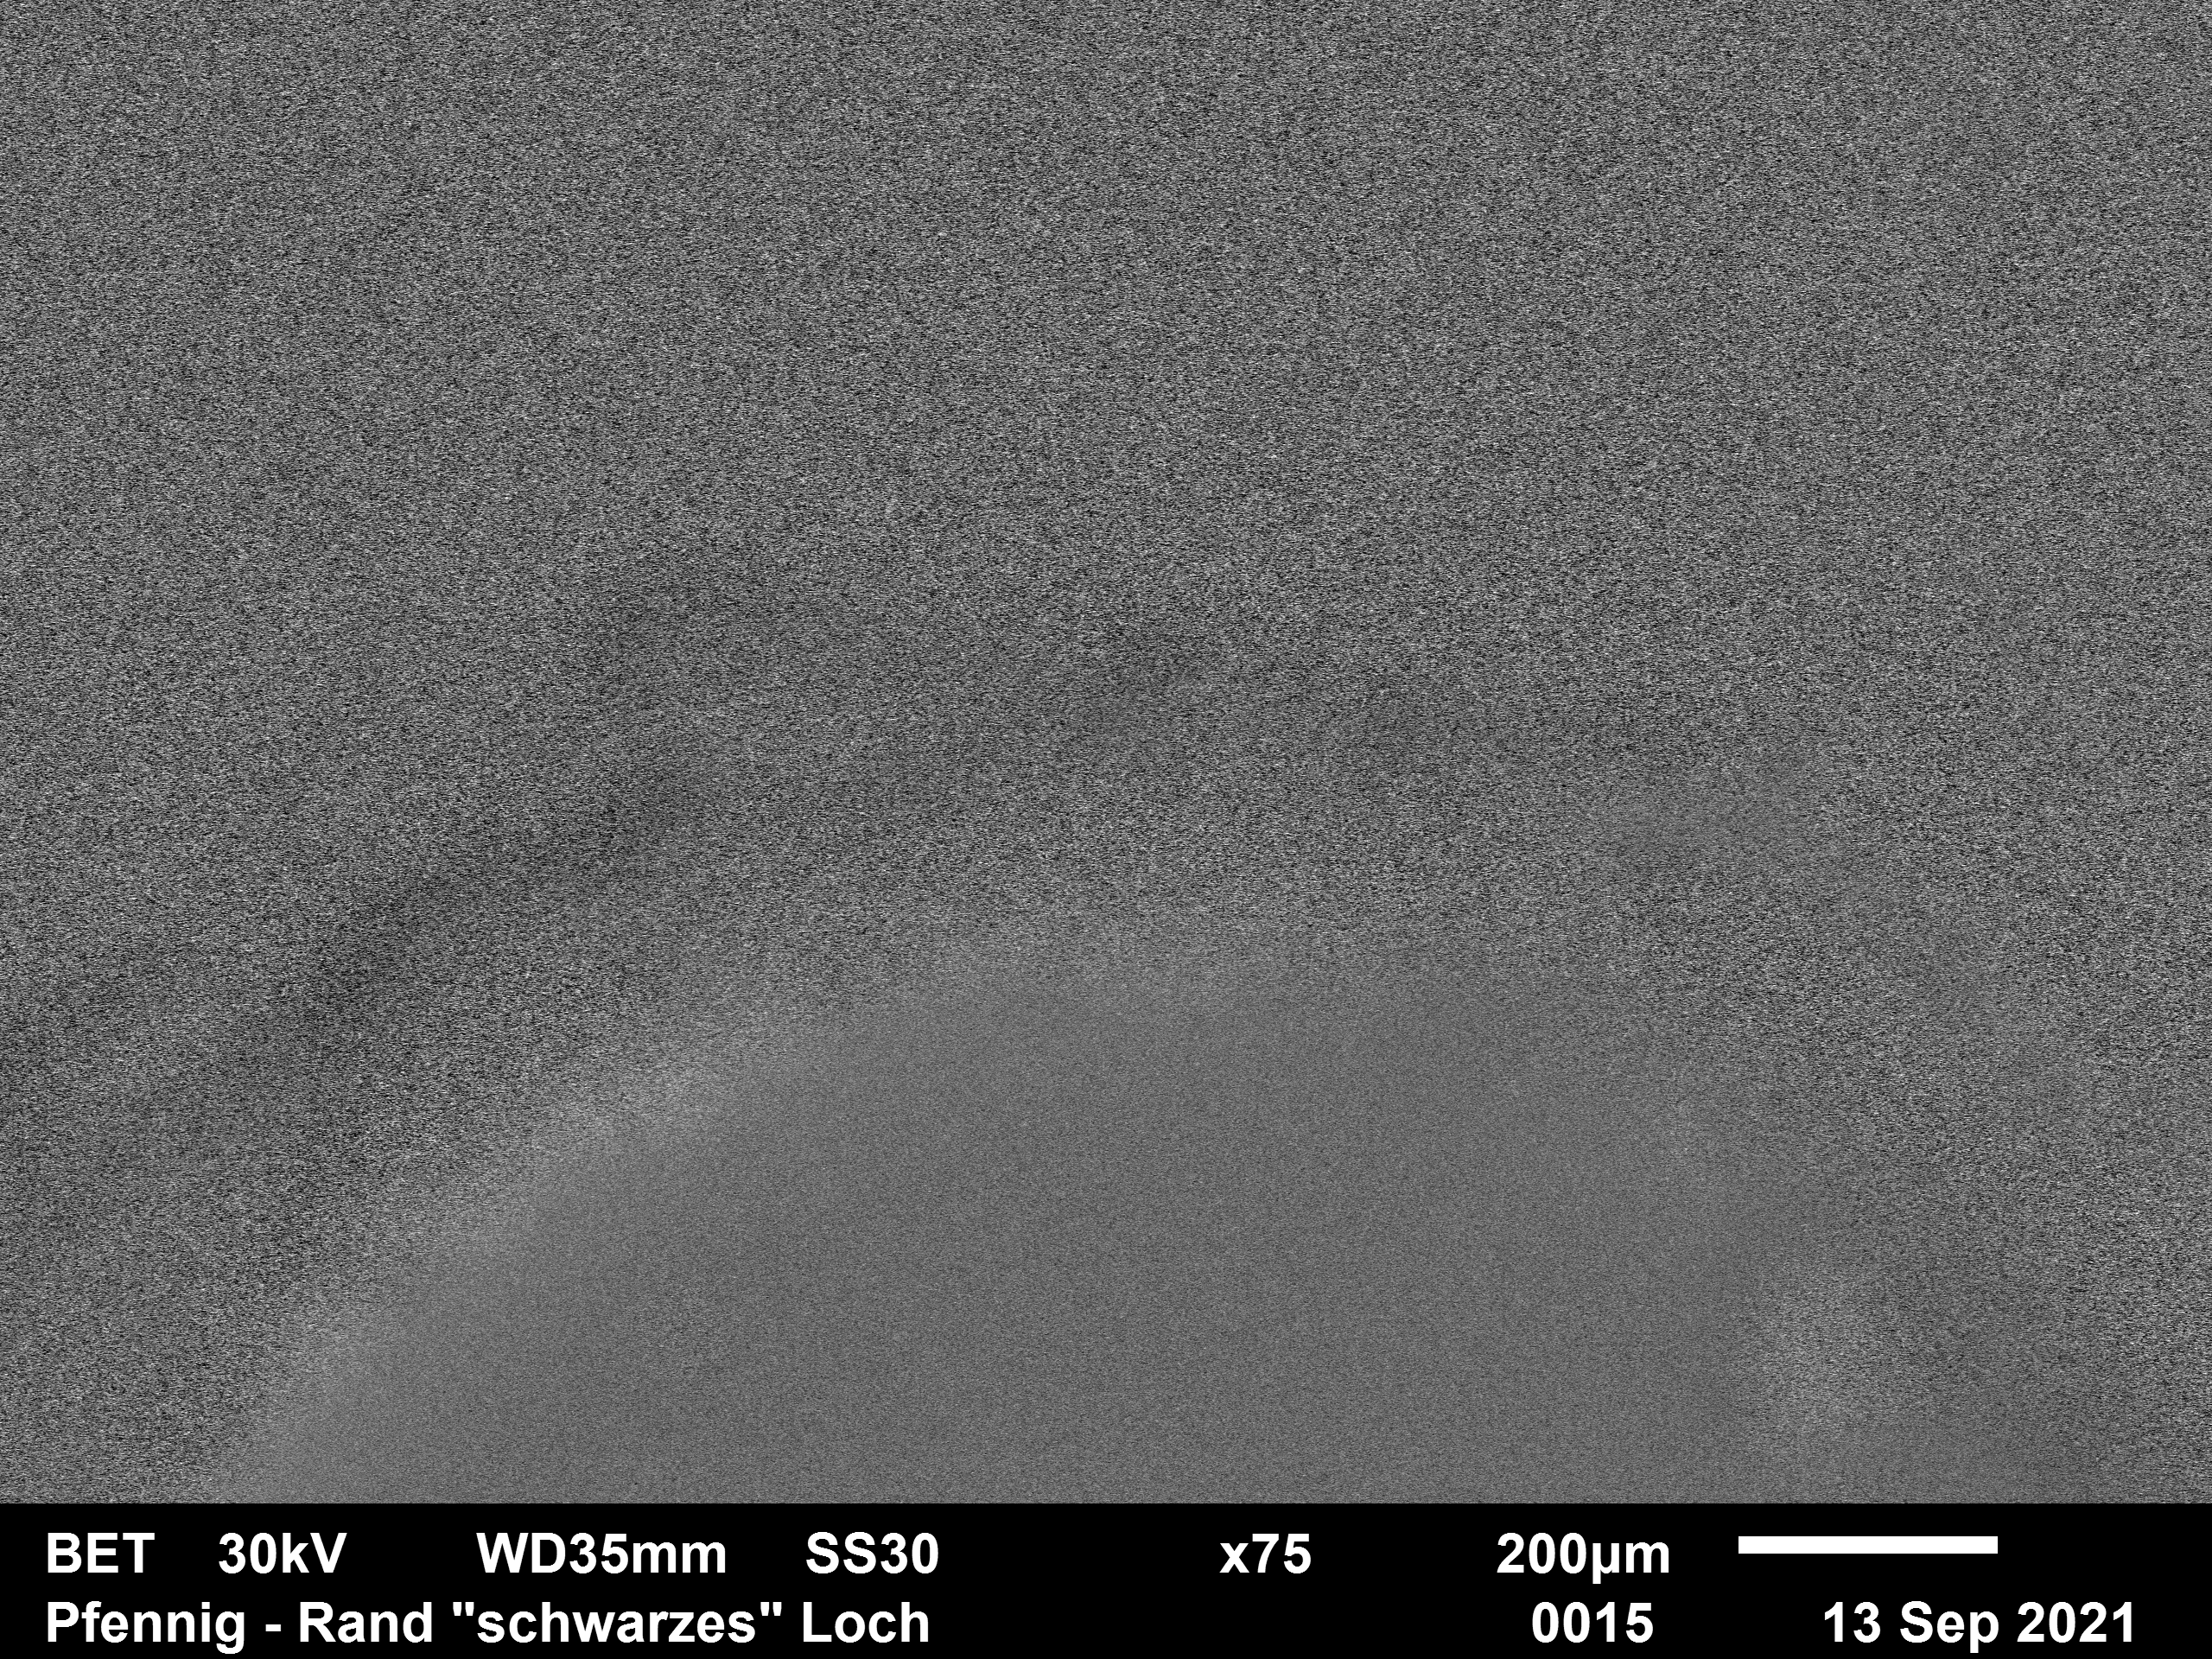
\includegraphics[width=\textwidth]{Auswertung/A/0015.png}
        \caption{$U_B = 30$ kV}
    \end{subfigure}
    
    \caption{BET bei unterschiedlichen Beschleunigunsspannungen}
\end{figure}

Für die Bilder im BET Modus lassen sich wenig Aussagen machen, da die Bildqualität im Allgemeinen sehr schlecht ist. Es lassen sich nur kannten erkennen, was im Topo-Mode keine Überraschung ist. Außerdem liegt die Vermutung nahe, dass die Einstellung des Fokus für $U_B = 30$ kV nicht optimal gewählt wurde. Unserer Vermutung nach müssten die Kannten für größeren Energie beim PE Strahl besser zu erkennen sein.

\newpage
Außerdem wurde eine Stelle mit verschiedenen Strahldurschmessern abgetastet.
\begin{figure}[h]
    \centering
    
    \begin{subfigure}[b]{0.45\textwidth}
        \centering
        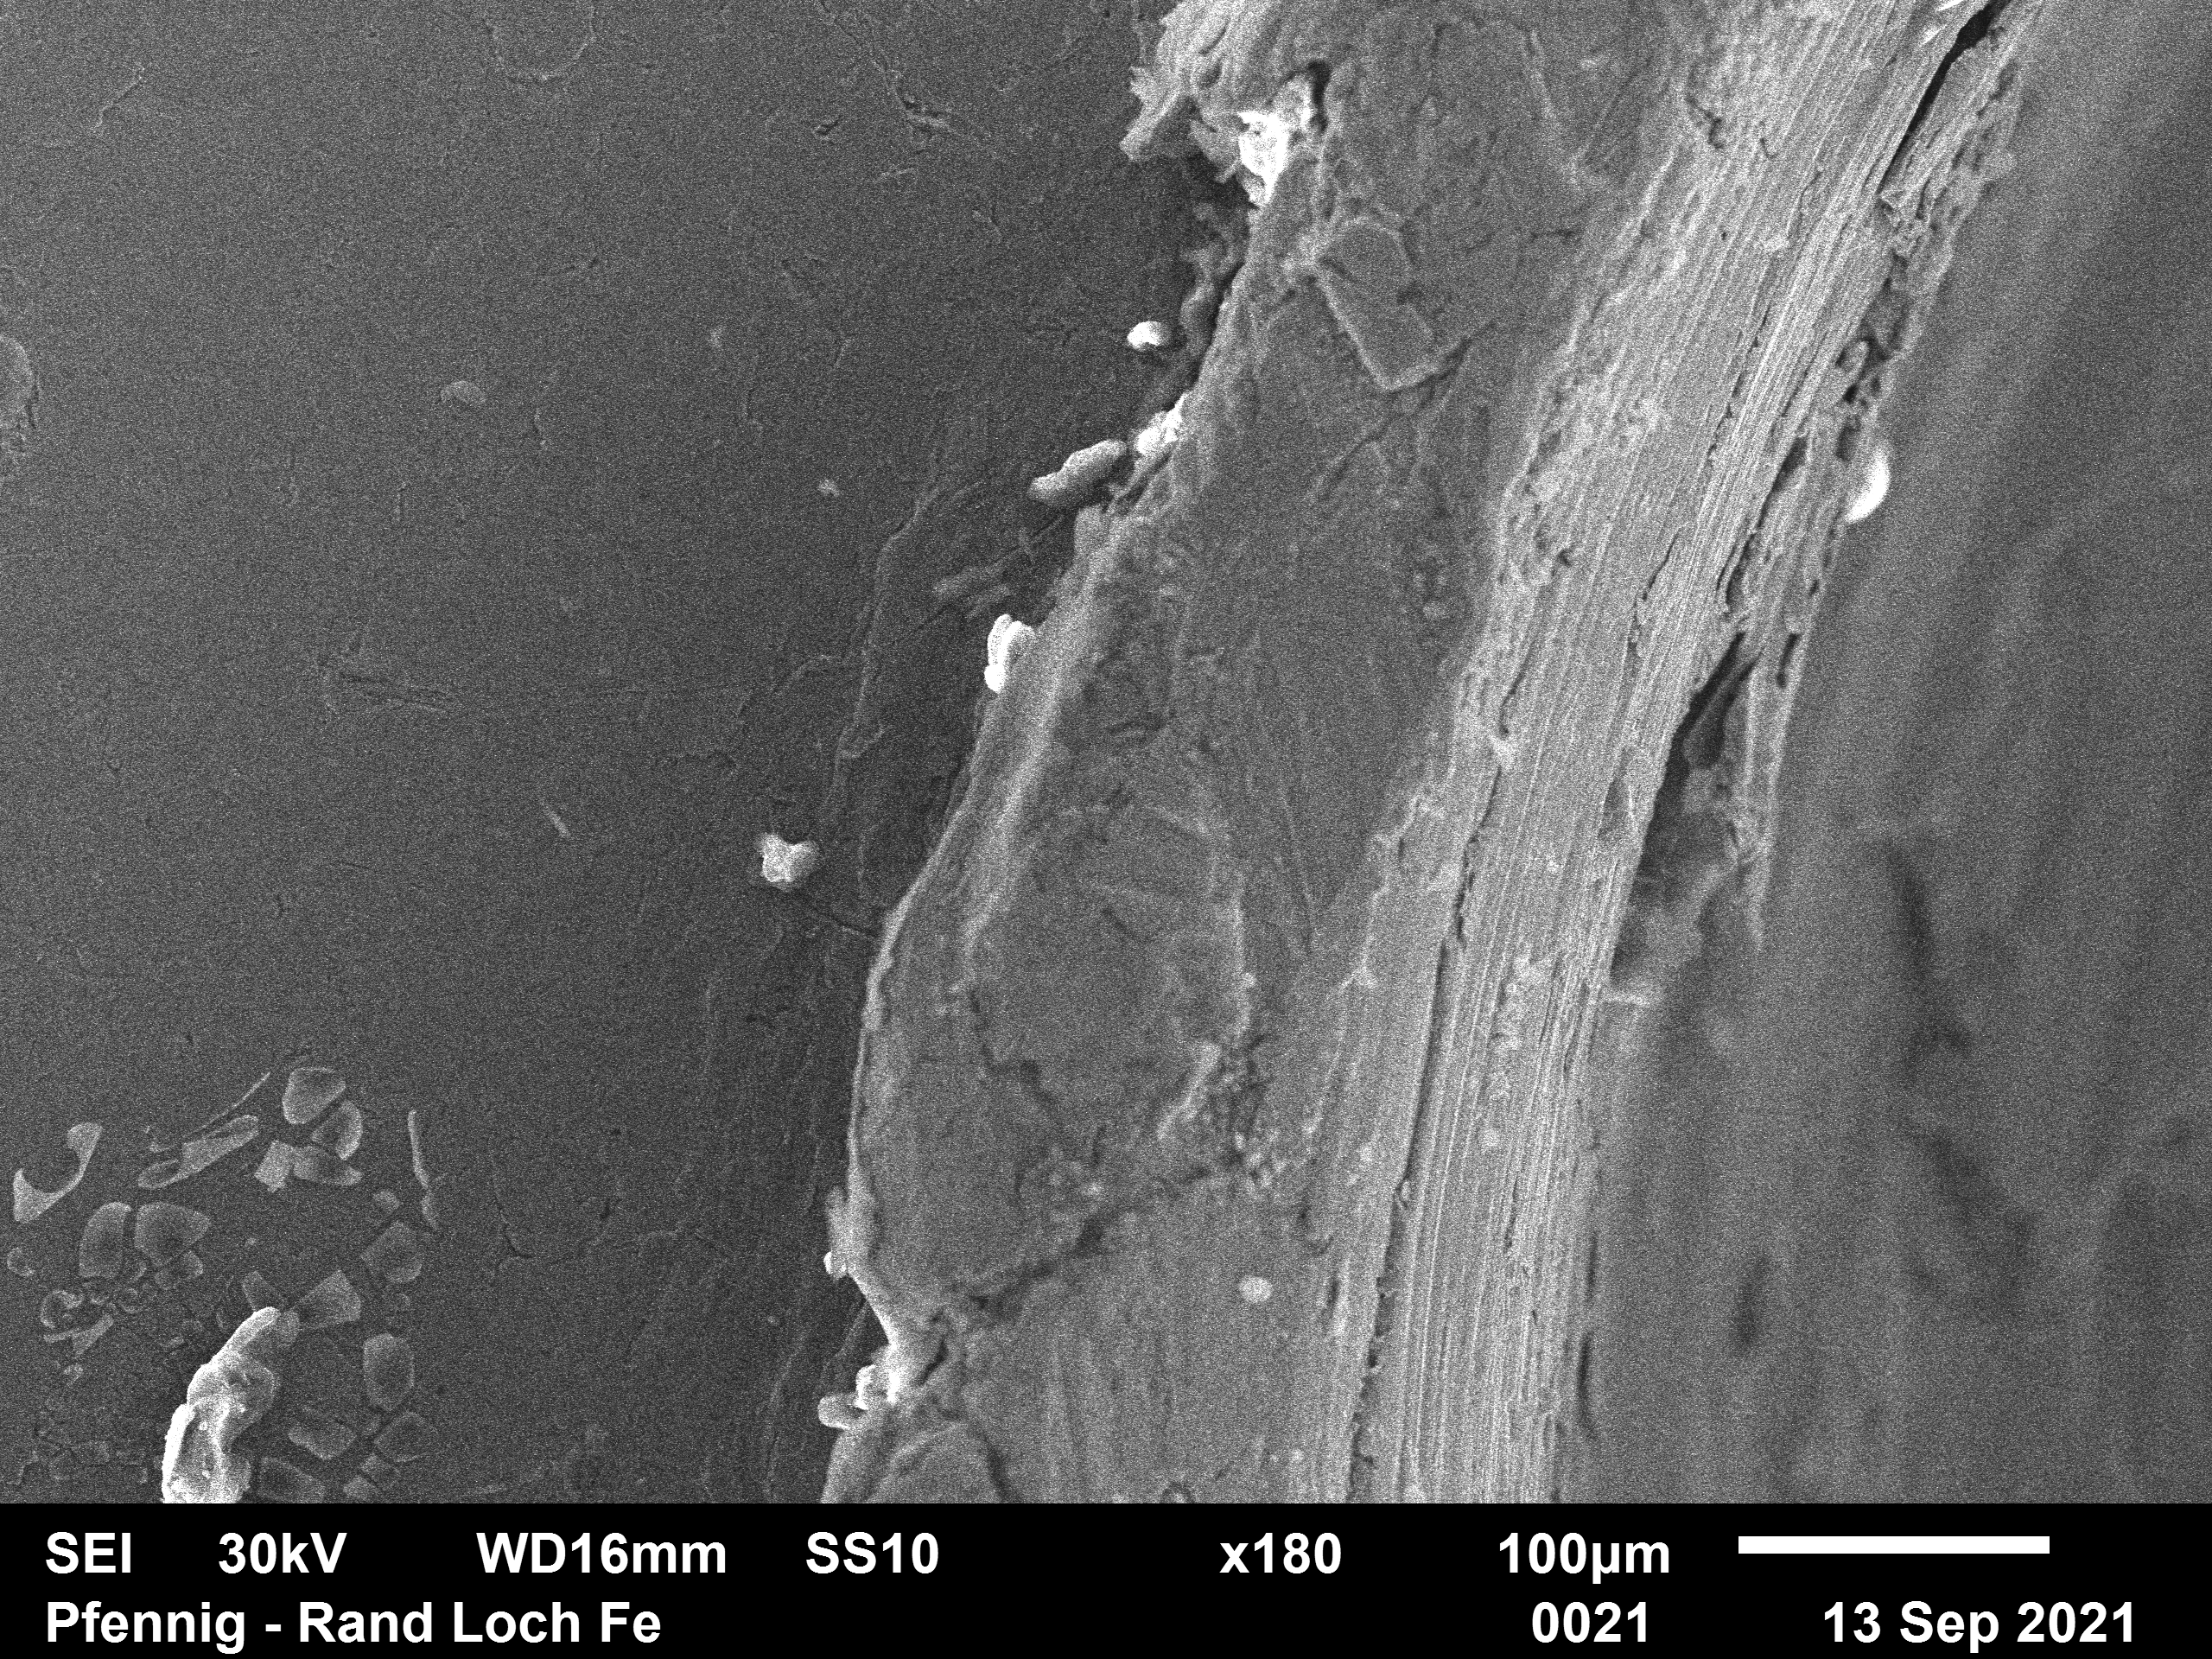
\includegraphics[width=\textwidth]{Auswertung/A/0021.png}
        \caption{SS 10}
    \end{subfigure}
    \hfill
    \begin{subfigure}[b]{0.45\textwidth}
        \centering
        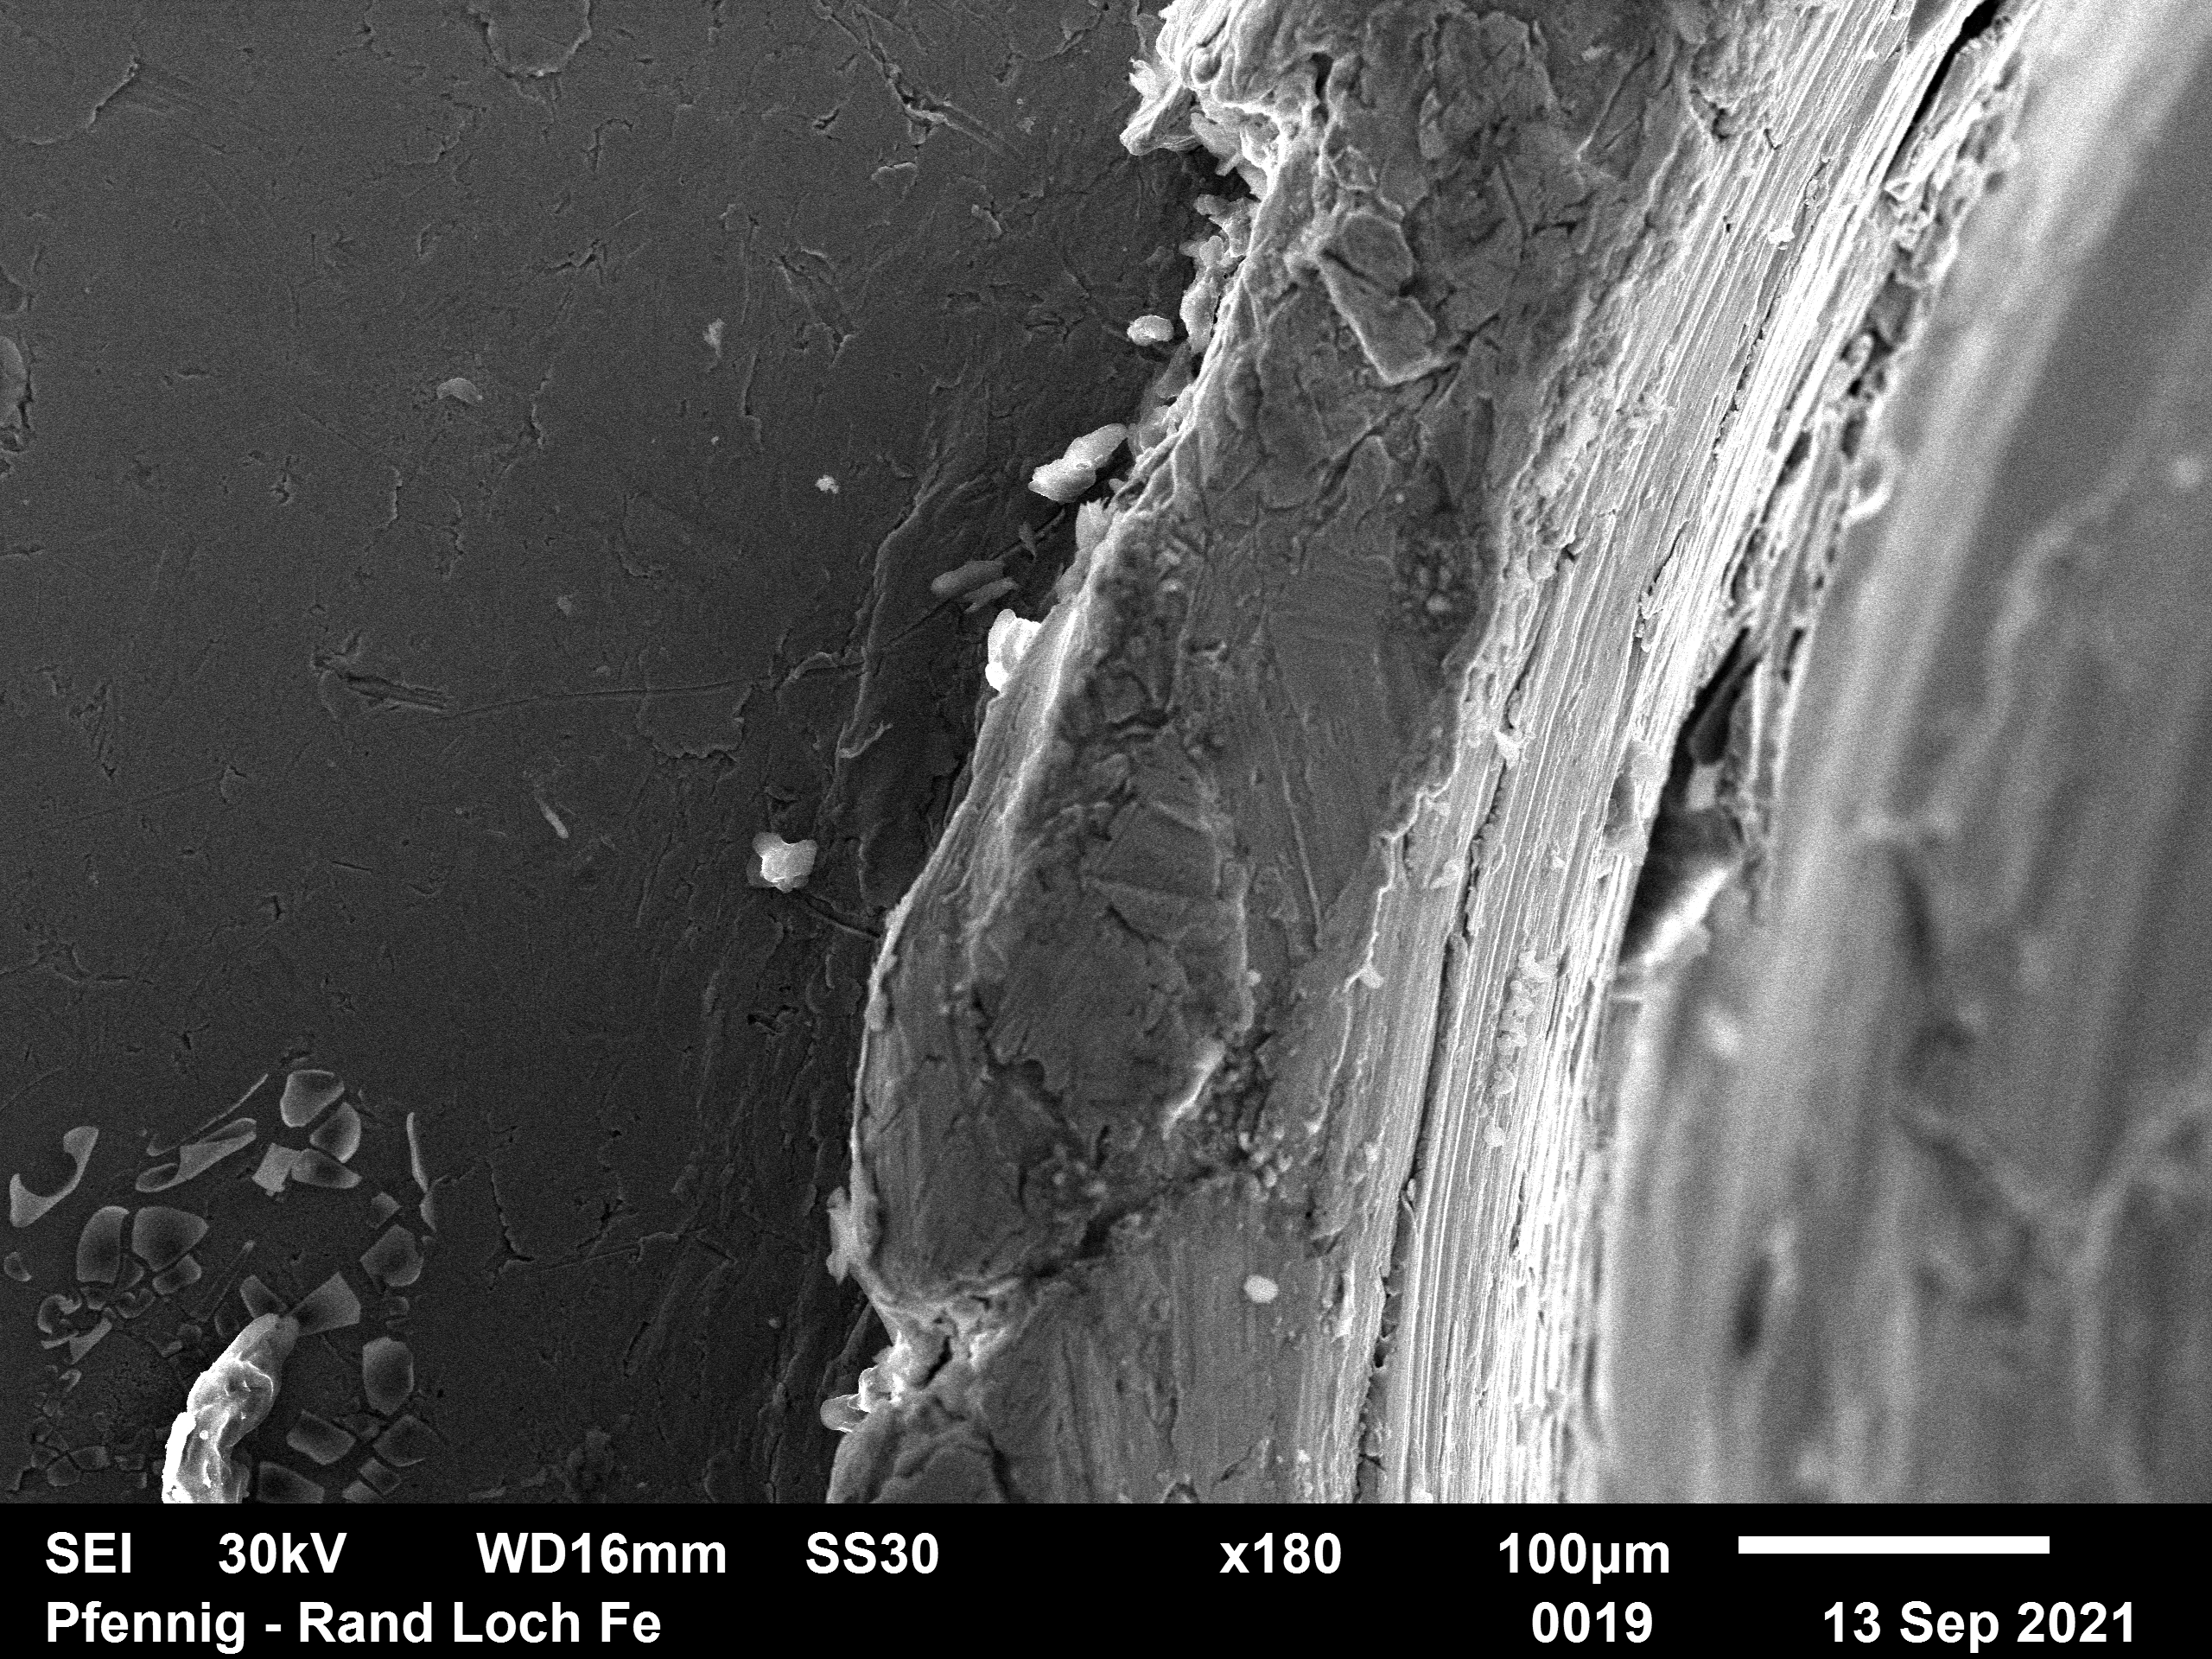
\includegraphics[width=\textwidth]{Auswertung/A/0019.png}
        \caption{SS 30}
    \end{subfigure}
    \\
    \begin{subfigure}[b]{0.45\textwidth}
        \centering
        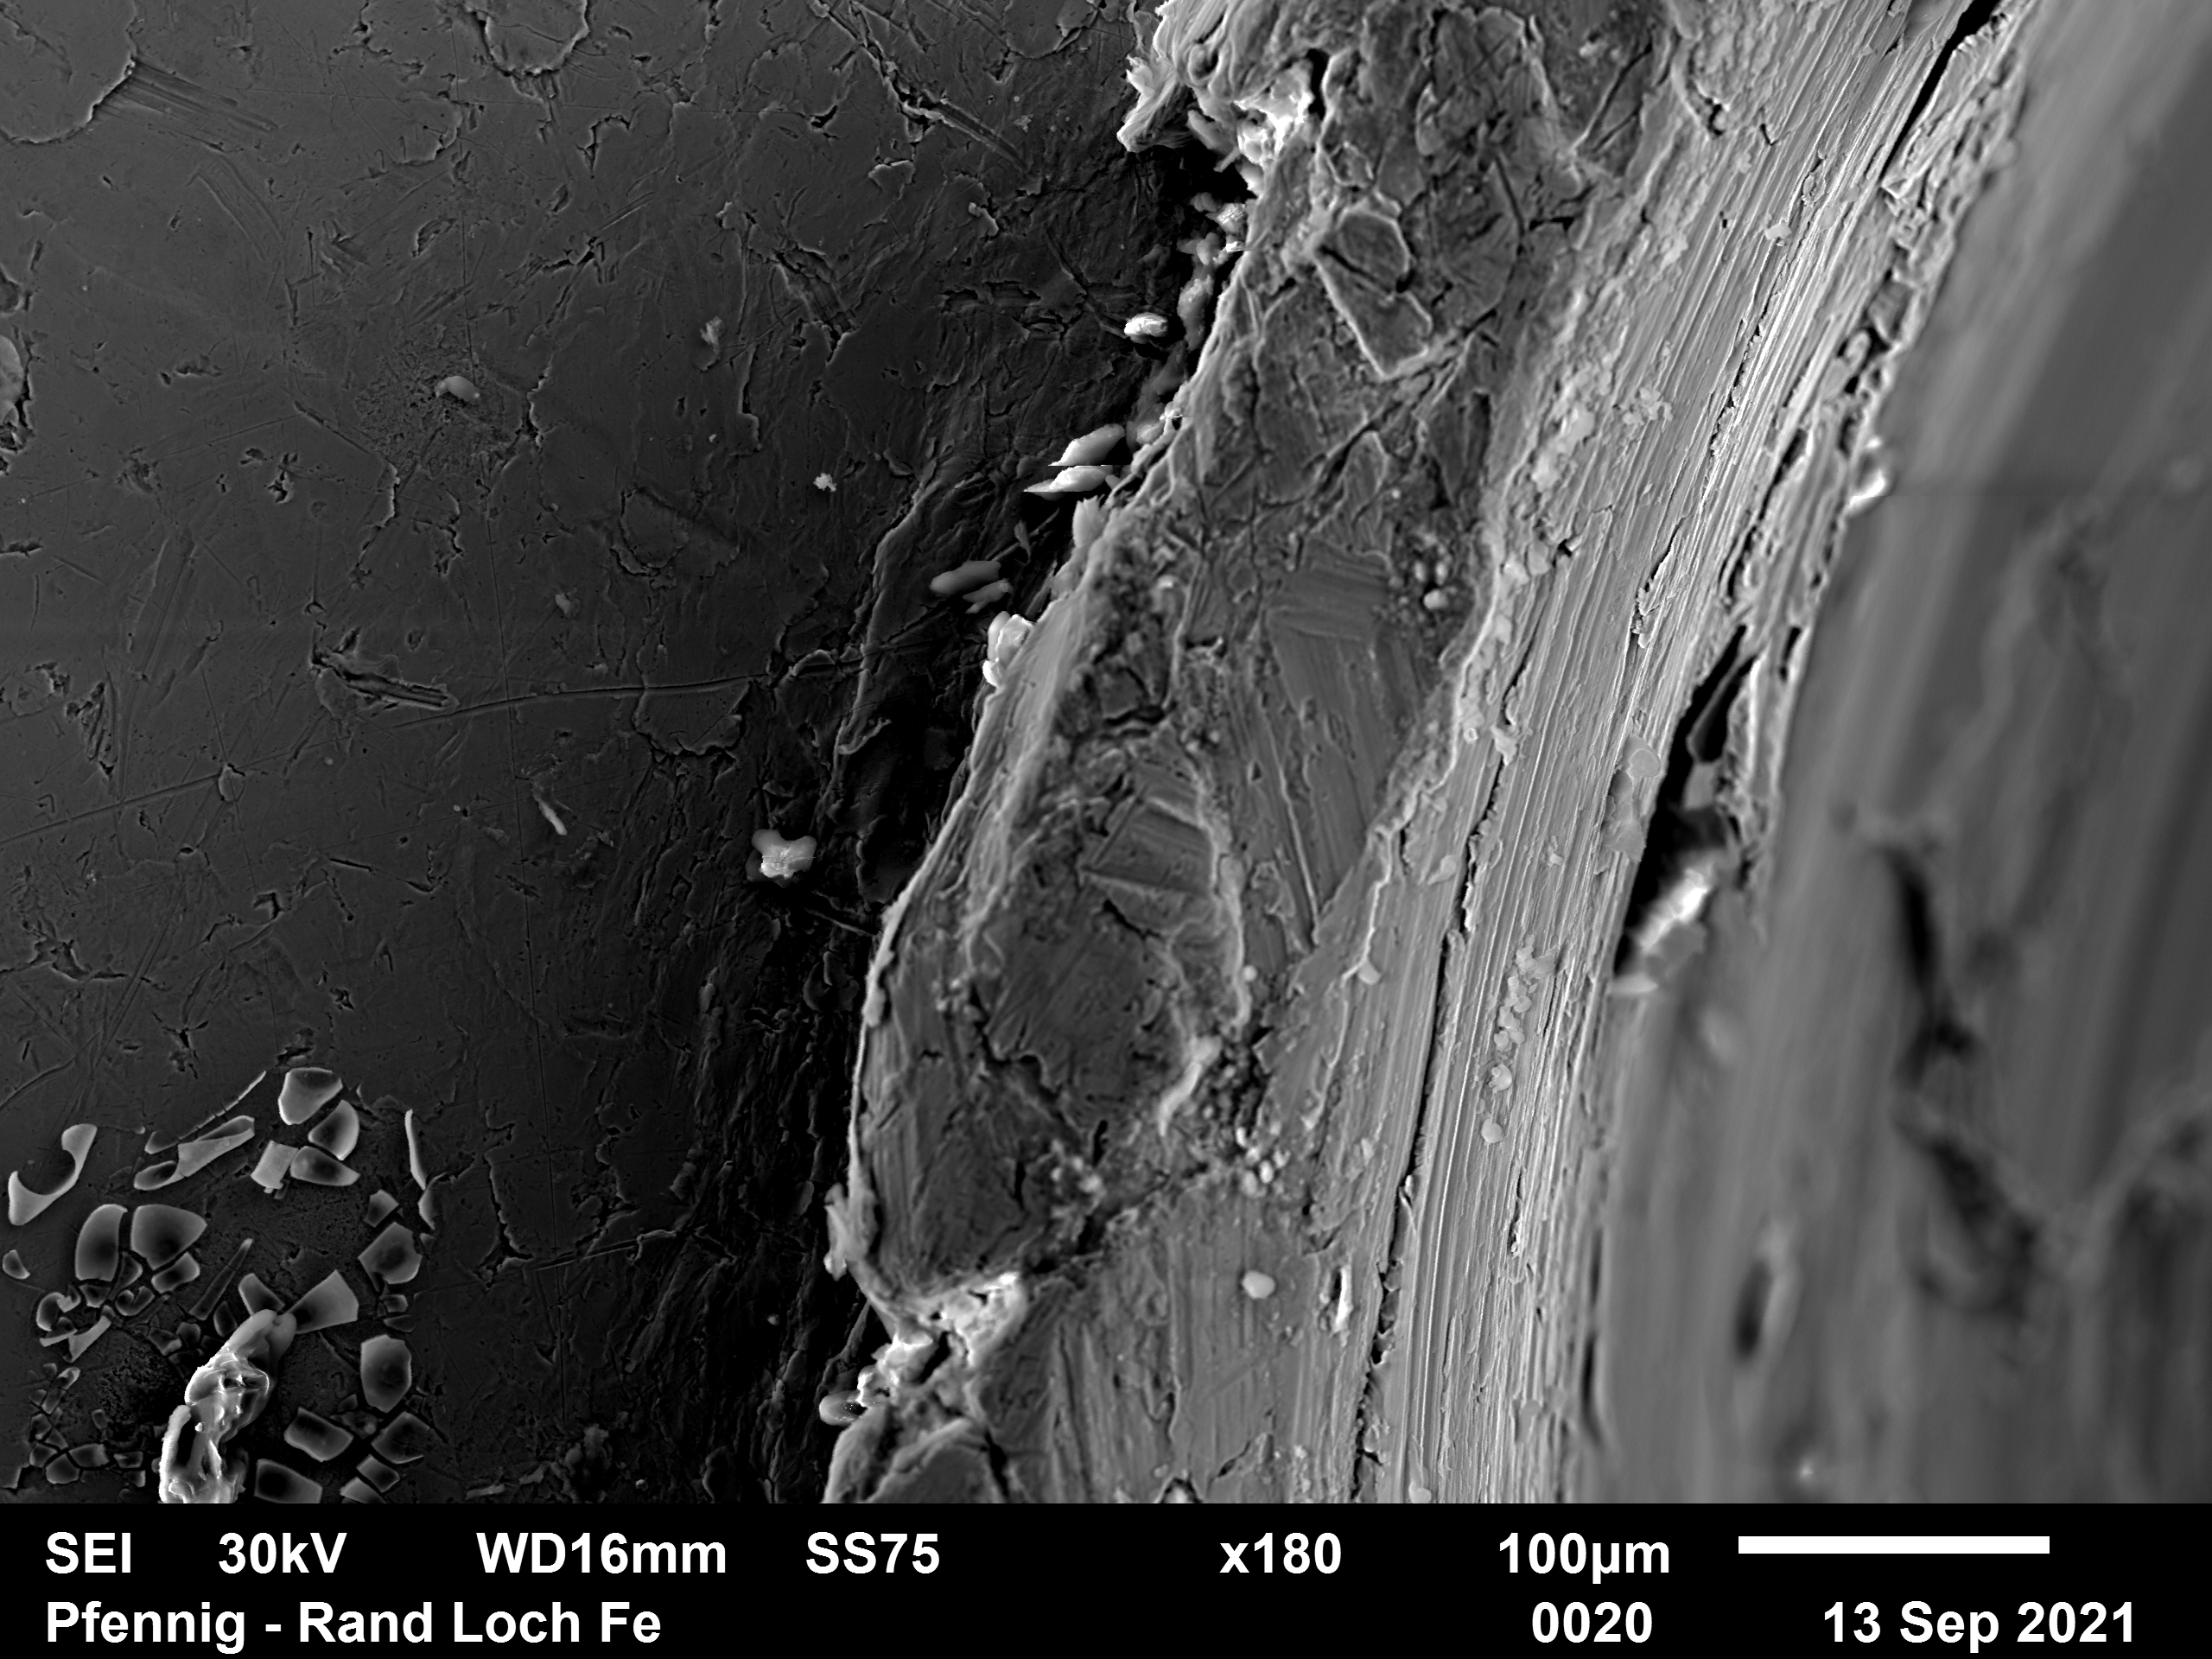
\includegraphics[width=\textwidth]{Auswertung/A/0020.png}
        \caption{SS 75}
    \end{subfigure}
    \caption{SEI bei unterschiedlichen Strahldurschmessern}
\end{figure}

Hier fällt auf, dass die Bilder mit abnehmenden SS körniger werden und somit auch weniger Details zu erkennen sind.

\newpage
\subsection*{EDX Analyse}

Nun sollen das Röntgenspektrum der Münze, sowie des gefüllten Lochs mithilfe des EDX Detektors aufgezeichnet werden. Mit dessen Hilfe kann die Materialzusammensetzung ermittelt werden. \\

Zuerst wurde das Spektrum der Münze aufgenommen: 
\begin{figure}[h]
    \centering
    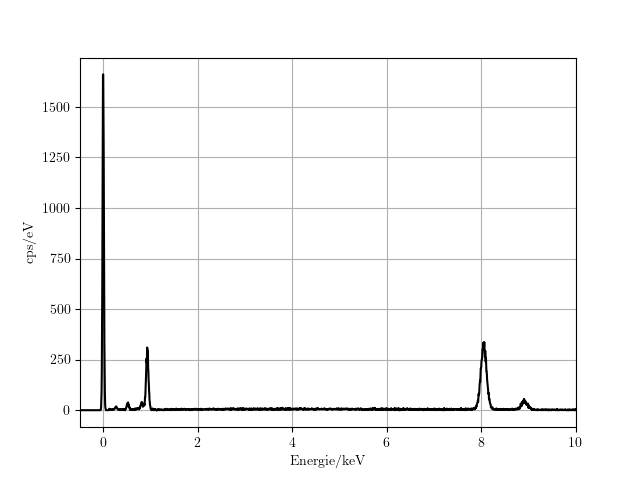
\includegraphics[width=\textwidth]{Auswertung/A/EdxFl.png}
    \caption{Röntgenspektrum der Kupfermünze}
\end{figure}

Die EDX Analyse wird weitestgehend automatisch vom Computer übernommen. Nach aktivierung der Messung wird ein Röntgenspektrum aufgezeichnet. Anhand der Peaks werden die enthaltenen Elemente bestimmt und anhand der Intensität dieser wird die Konzentration der jeweiligen Stoffe durch den PC ermittelt.

\begin{table}[h]
    \centering
    \begin{tabular}{c|c|c|c|c|c|c}
        Element & OZ &Serie& unn. C & norm. C &  Atom. C  & Fehler (1 Sigma) \\
         & & & [Gew. \%] & [Gew. \%] & [At. \%] & [Gew. \%] \\
        \hline\hline
        C & 6 & K & 13,96&11,87&23,84 & 35,27\\
        O & 8 & K & 10,72&9,11&20,33 & 3,41\\
        Cu & 29 & K & 92,94&79,02&44,40 & 2,50\\
    \end{tabular}
    \caption{Ergebnisse der EDX-Analyse der Kupfermünze}
\end{table}

Nach der Analyse geht klar hervor das Kupfer den größten Anteil ausmacht, was bei einer Kupfermünze alles andere als verwunderlich ist. Die Übrigen Bestandteile, Kohlenstoff und Sauerstoff, sind wohl auf Organische verunreinigungen zurück zuführen.

\newpage
Anschließend wurde das Spektrum des Materials in einem der Löcher aufgenommen: 
\begin{figure}[h]
    \centering
    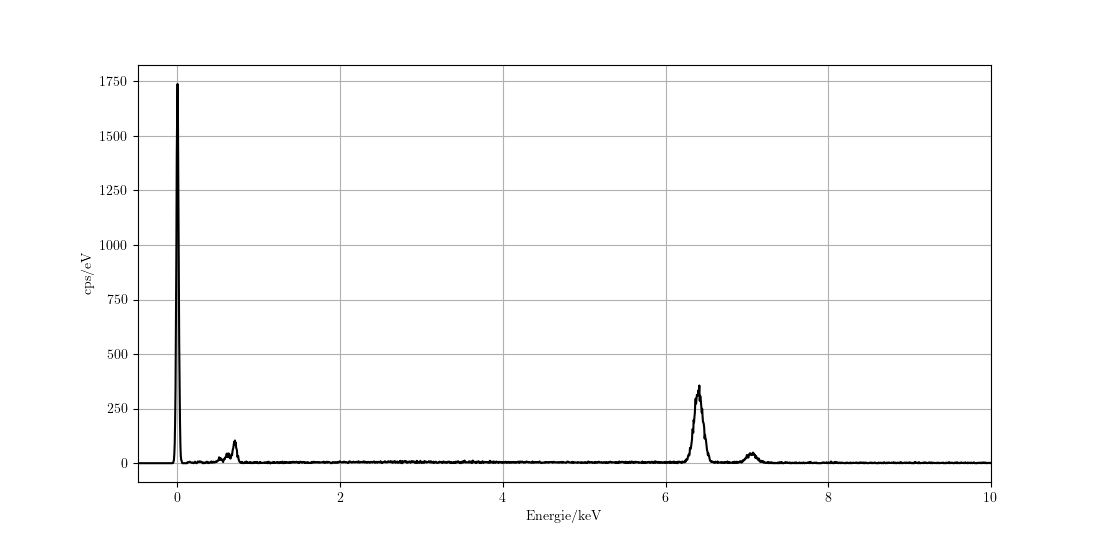
\includegraphics[width=\textwidth]{Auswertung/A/EdxLoch.png}
    \caption{Röntgenspektrum des Fremdmaterials}
\end{figure}


\begin{table}[h]
    \centering
    \begin{tabular}{c|c|c|c|c|c|c}
        Element & OZ &Serie& unn. C & norm. C &  Atom. C  & Fehler (1 Sigma) \\
         & & & [Gew. \%] & [Gew. \%] & [At. \%] & [Gew. \%] \\
        \hline\hline
        C & 6 & K & 7,06&7,57&23,84 & 4,17\\
        O & 8 & K & 7,52&8,06&19,05 & 2,83\\
        Fe & 26 & K & 78,68&84,36&57,11 & 2,19\\
    \end{tabular}
    \caption{Ergebnisse der EDX-Analyse des Fremdmaterials}
\end{table}

Die Ergebnisse der Zweiten EDX Analyse sind hingegen wesentlich interessanter, wohingegen Kohlenstoff und Sauerstoff wieder auf organische kontamination hindeuten haben wir so herausgefunden, dass das Loch mit Eisen gefüllt wurde.

\newpage
\section{Fliege}

Als nächste Probe wurde eine Fliege eingelegt. Da es sich hierbei um organisches Material handelt wurde sie mit Gold bedampft, um eine Untersuchung möglich zu machen. Weiterhin ist darauf zu achten, die Beschleunigungsspannung nicht zu groß (ca. 10  kV) einzustellen, da die Probe sonst beschädigt werden kann. \\

Zuerst wurde die Flieg im Ganzen aufgenommen. Um dabei eine höhe Tiefenschärfe zu erreichen wurde ein großer Arbeitsabstand eingestellt.
\begin{figure}[h]
    \centering
    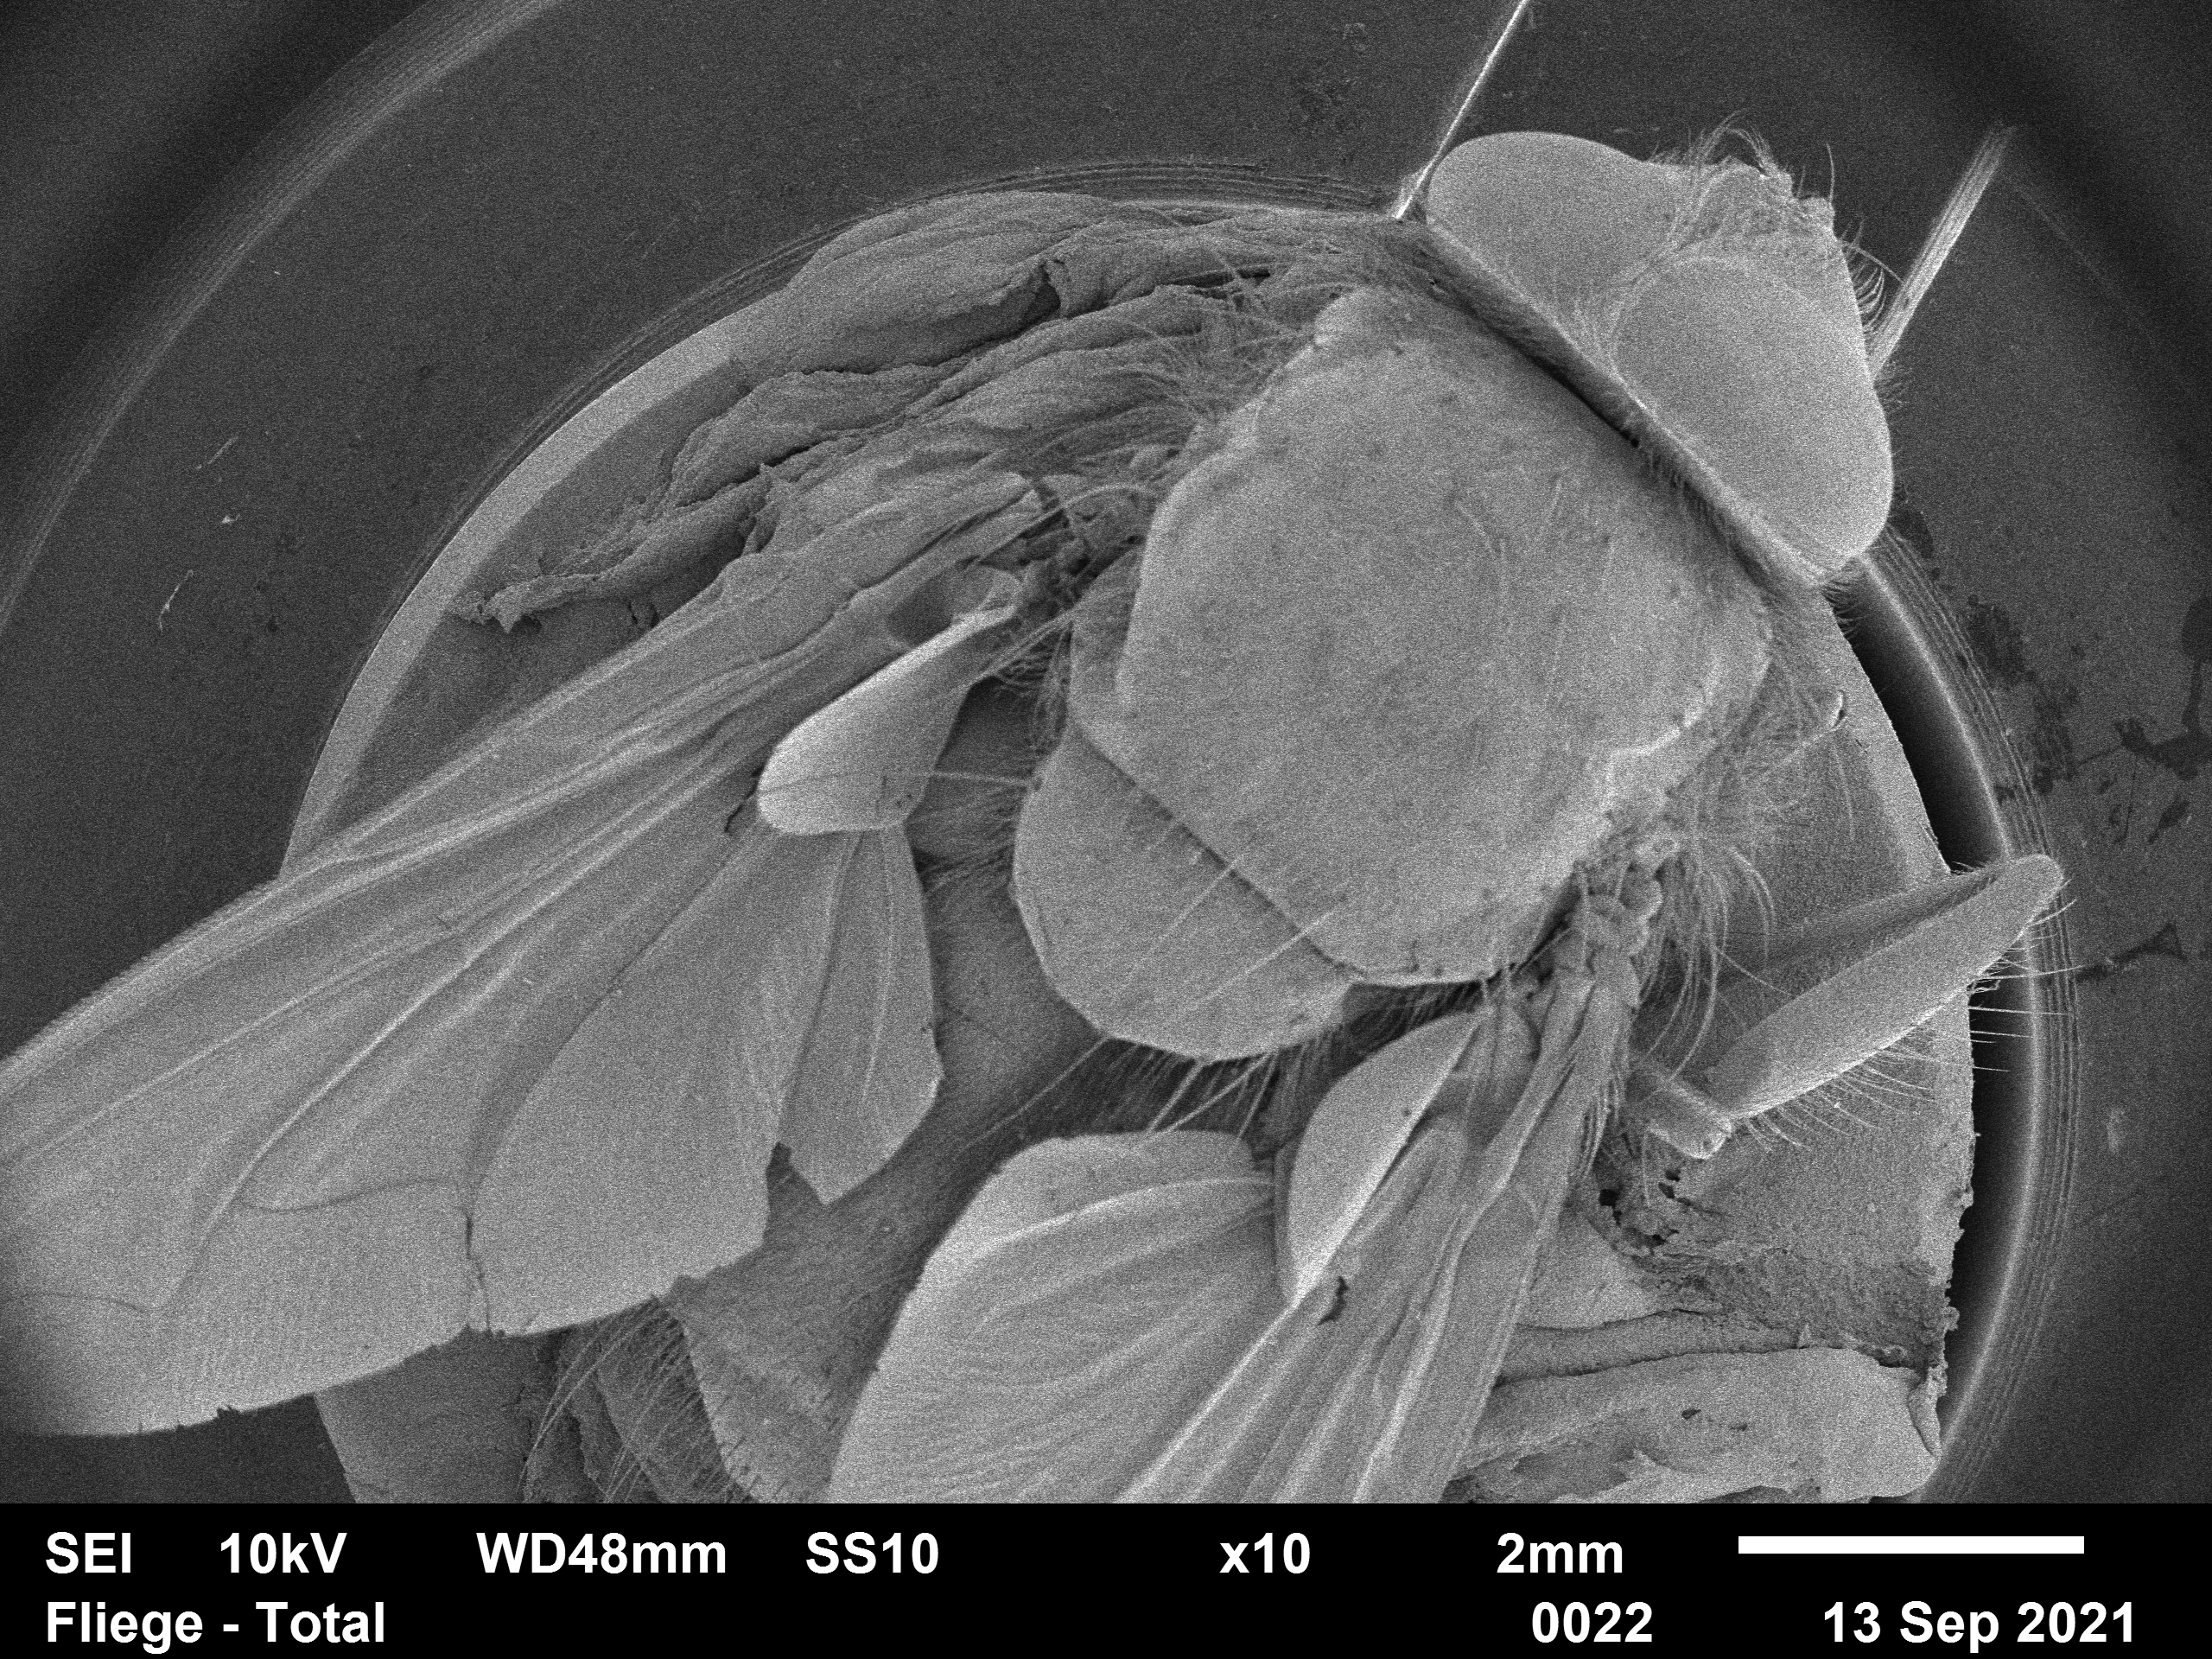
\includegraphics[width=\textwidth]{Auswertung/B/0022.png}
    \caption{Gesamtaufnahme der Fliege}
\end{figure}

\newpage
Als Nächstes wurde ein Segment des Facettenauges vermessen.
\begin{figure}[h]
    \centering
    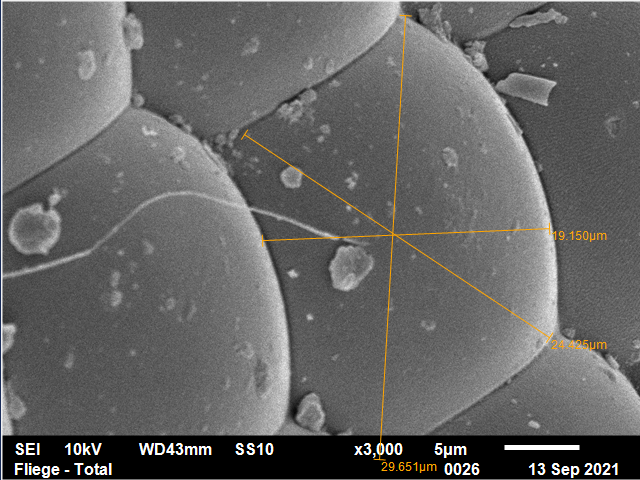
\includegraphics[width=\textwidth]{Auswertung/B/26-2.PNG}
    \caption{Segment eines Facettenauges der Fliege mit Bemaßung}
\end{figure}

Die größe der Segmente beläuft sich auf ca. 20 $\mu$m.

\newpage
\section{Zinnstandart}
In diesem Abschnitt sollen der Einfluss des Strahldurchmessers, der Beschleunigungsspannung und des Arbeitsabstands genauer beleuchtet werden. \\

Zuerst wird dazu der Strahldurchmesser variiert.
\begin{figure}[h]
    \centering
    \begin{subfigure}[b]{0.25\textwidth}
        \centering
        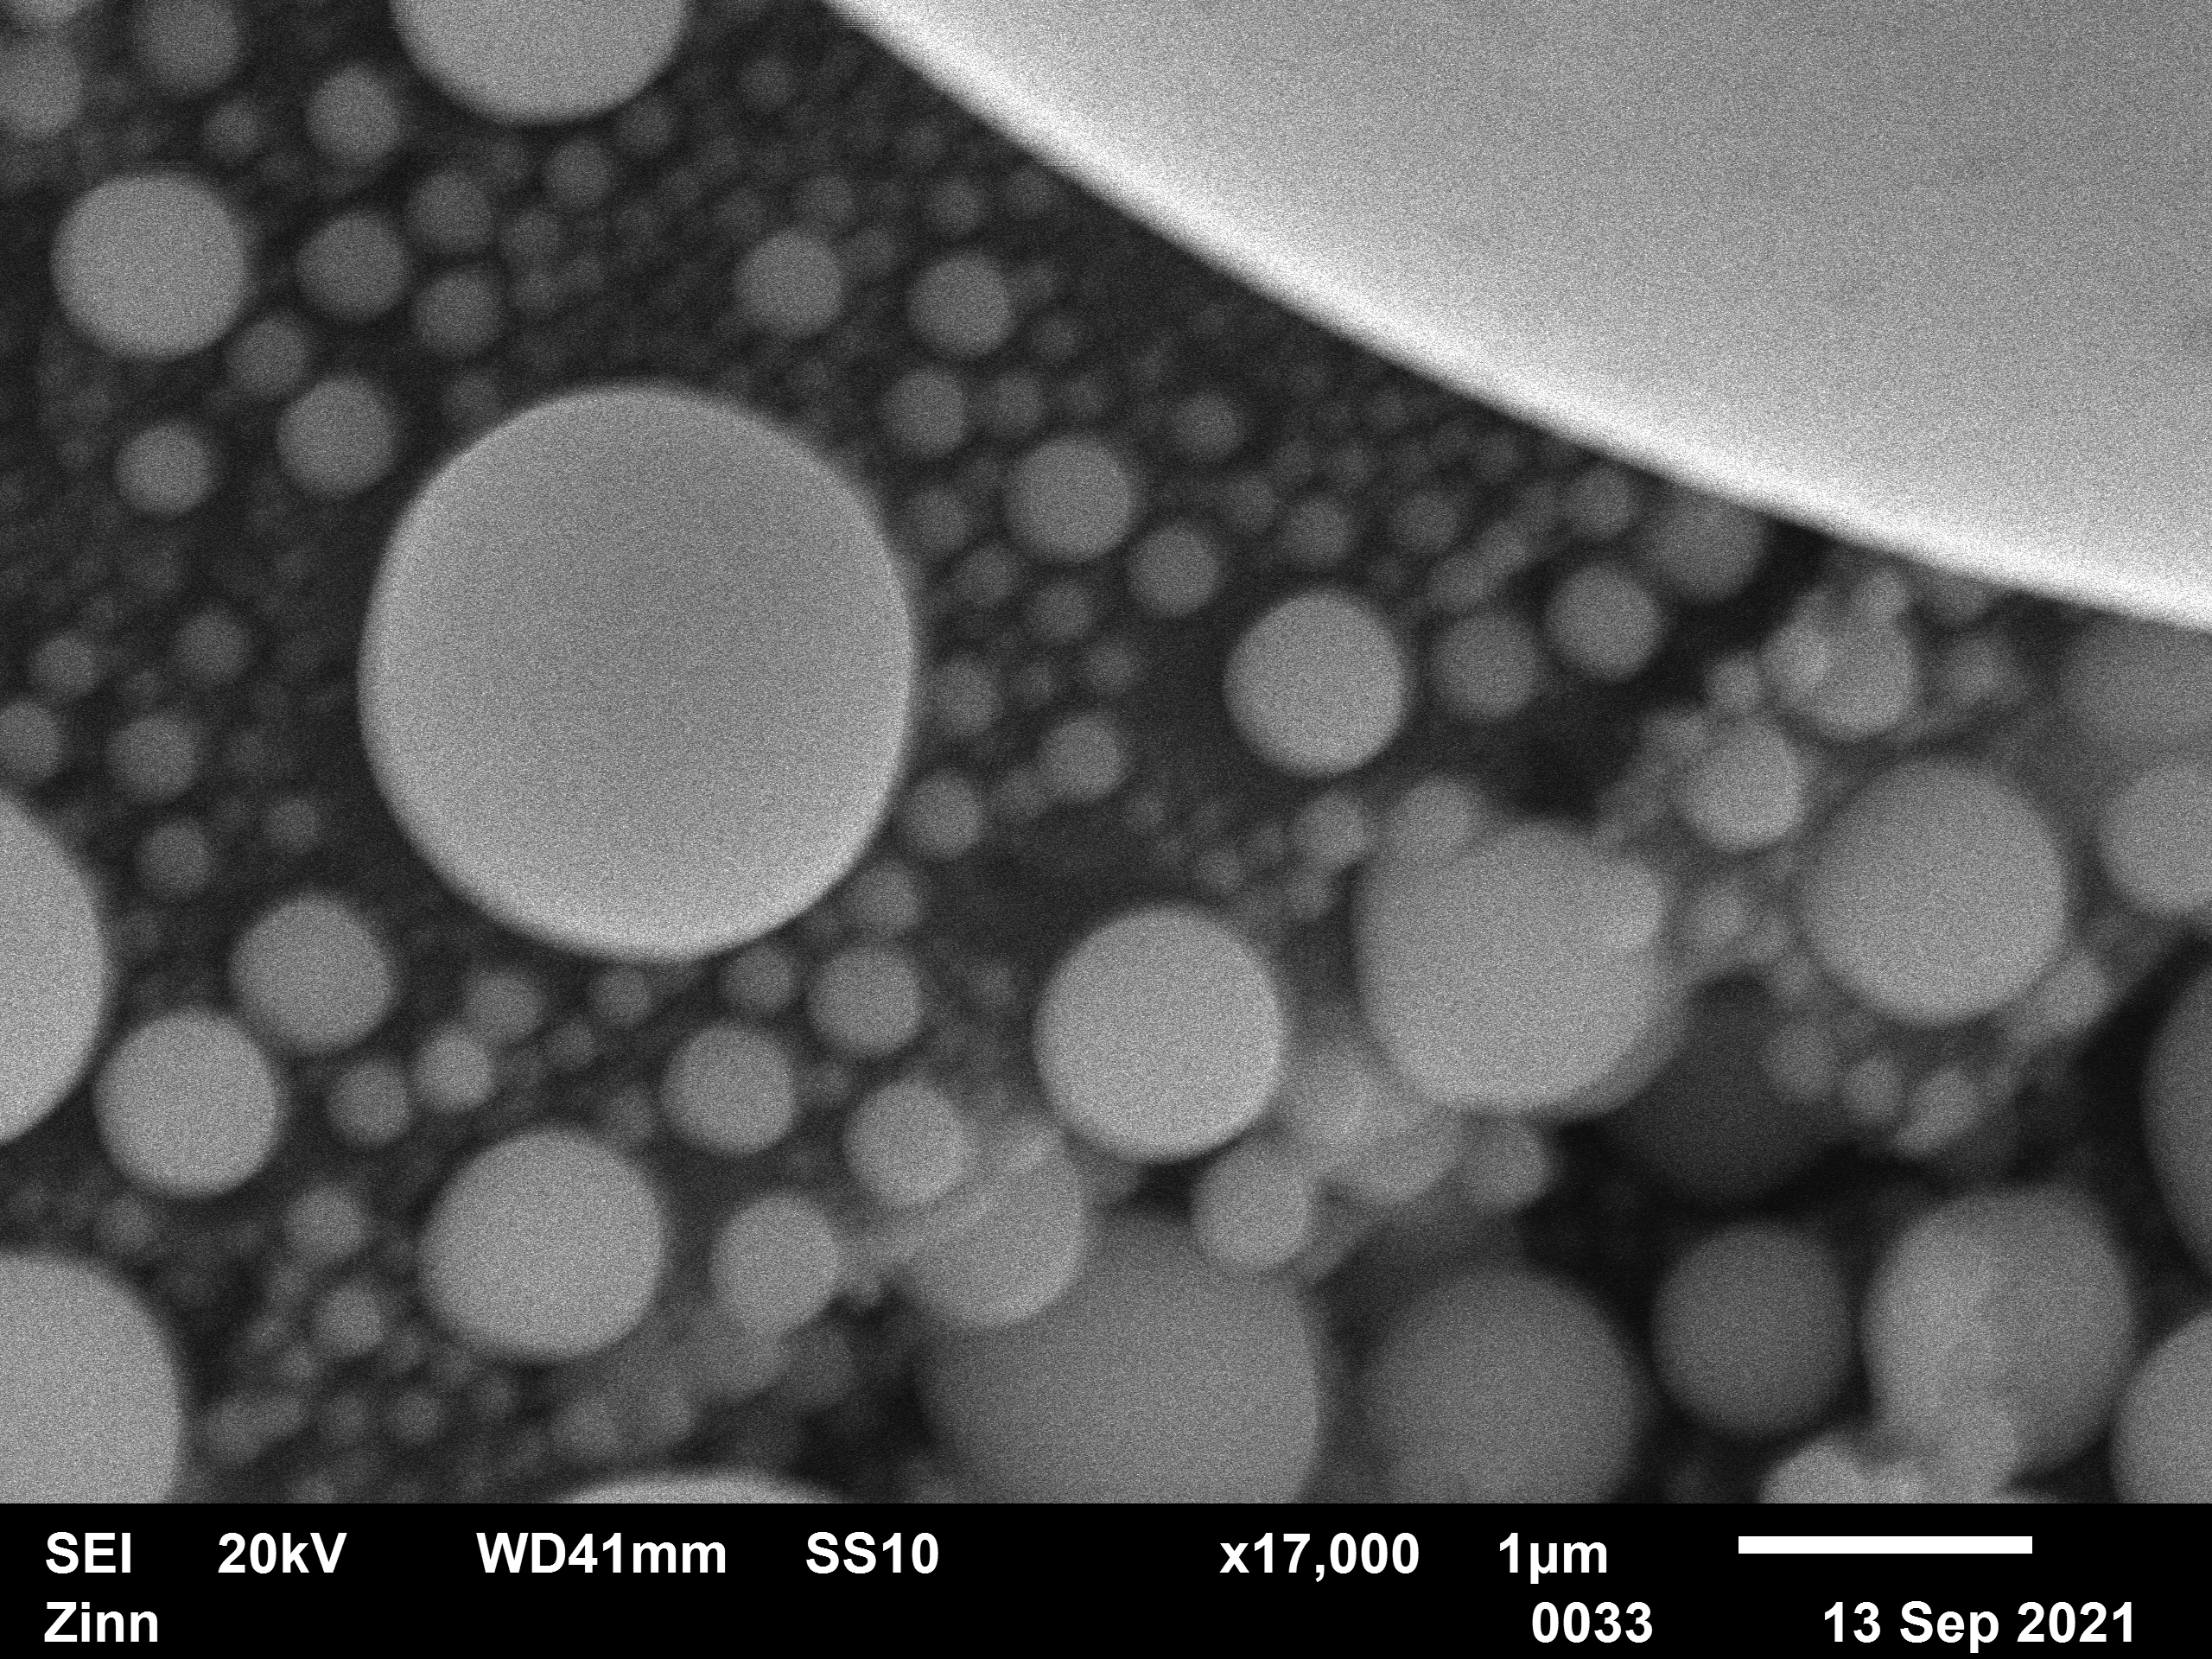
\includegraphics[width=\textwidth]{Auswertung/C/0033.png}
        \caption{SS 10}
    \end{subfigure}
    \hfill
    \begin{subfigure}[b]{0.25\textwidth}
        \centering
        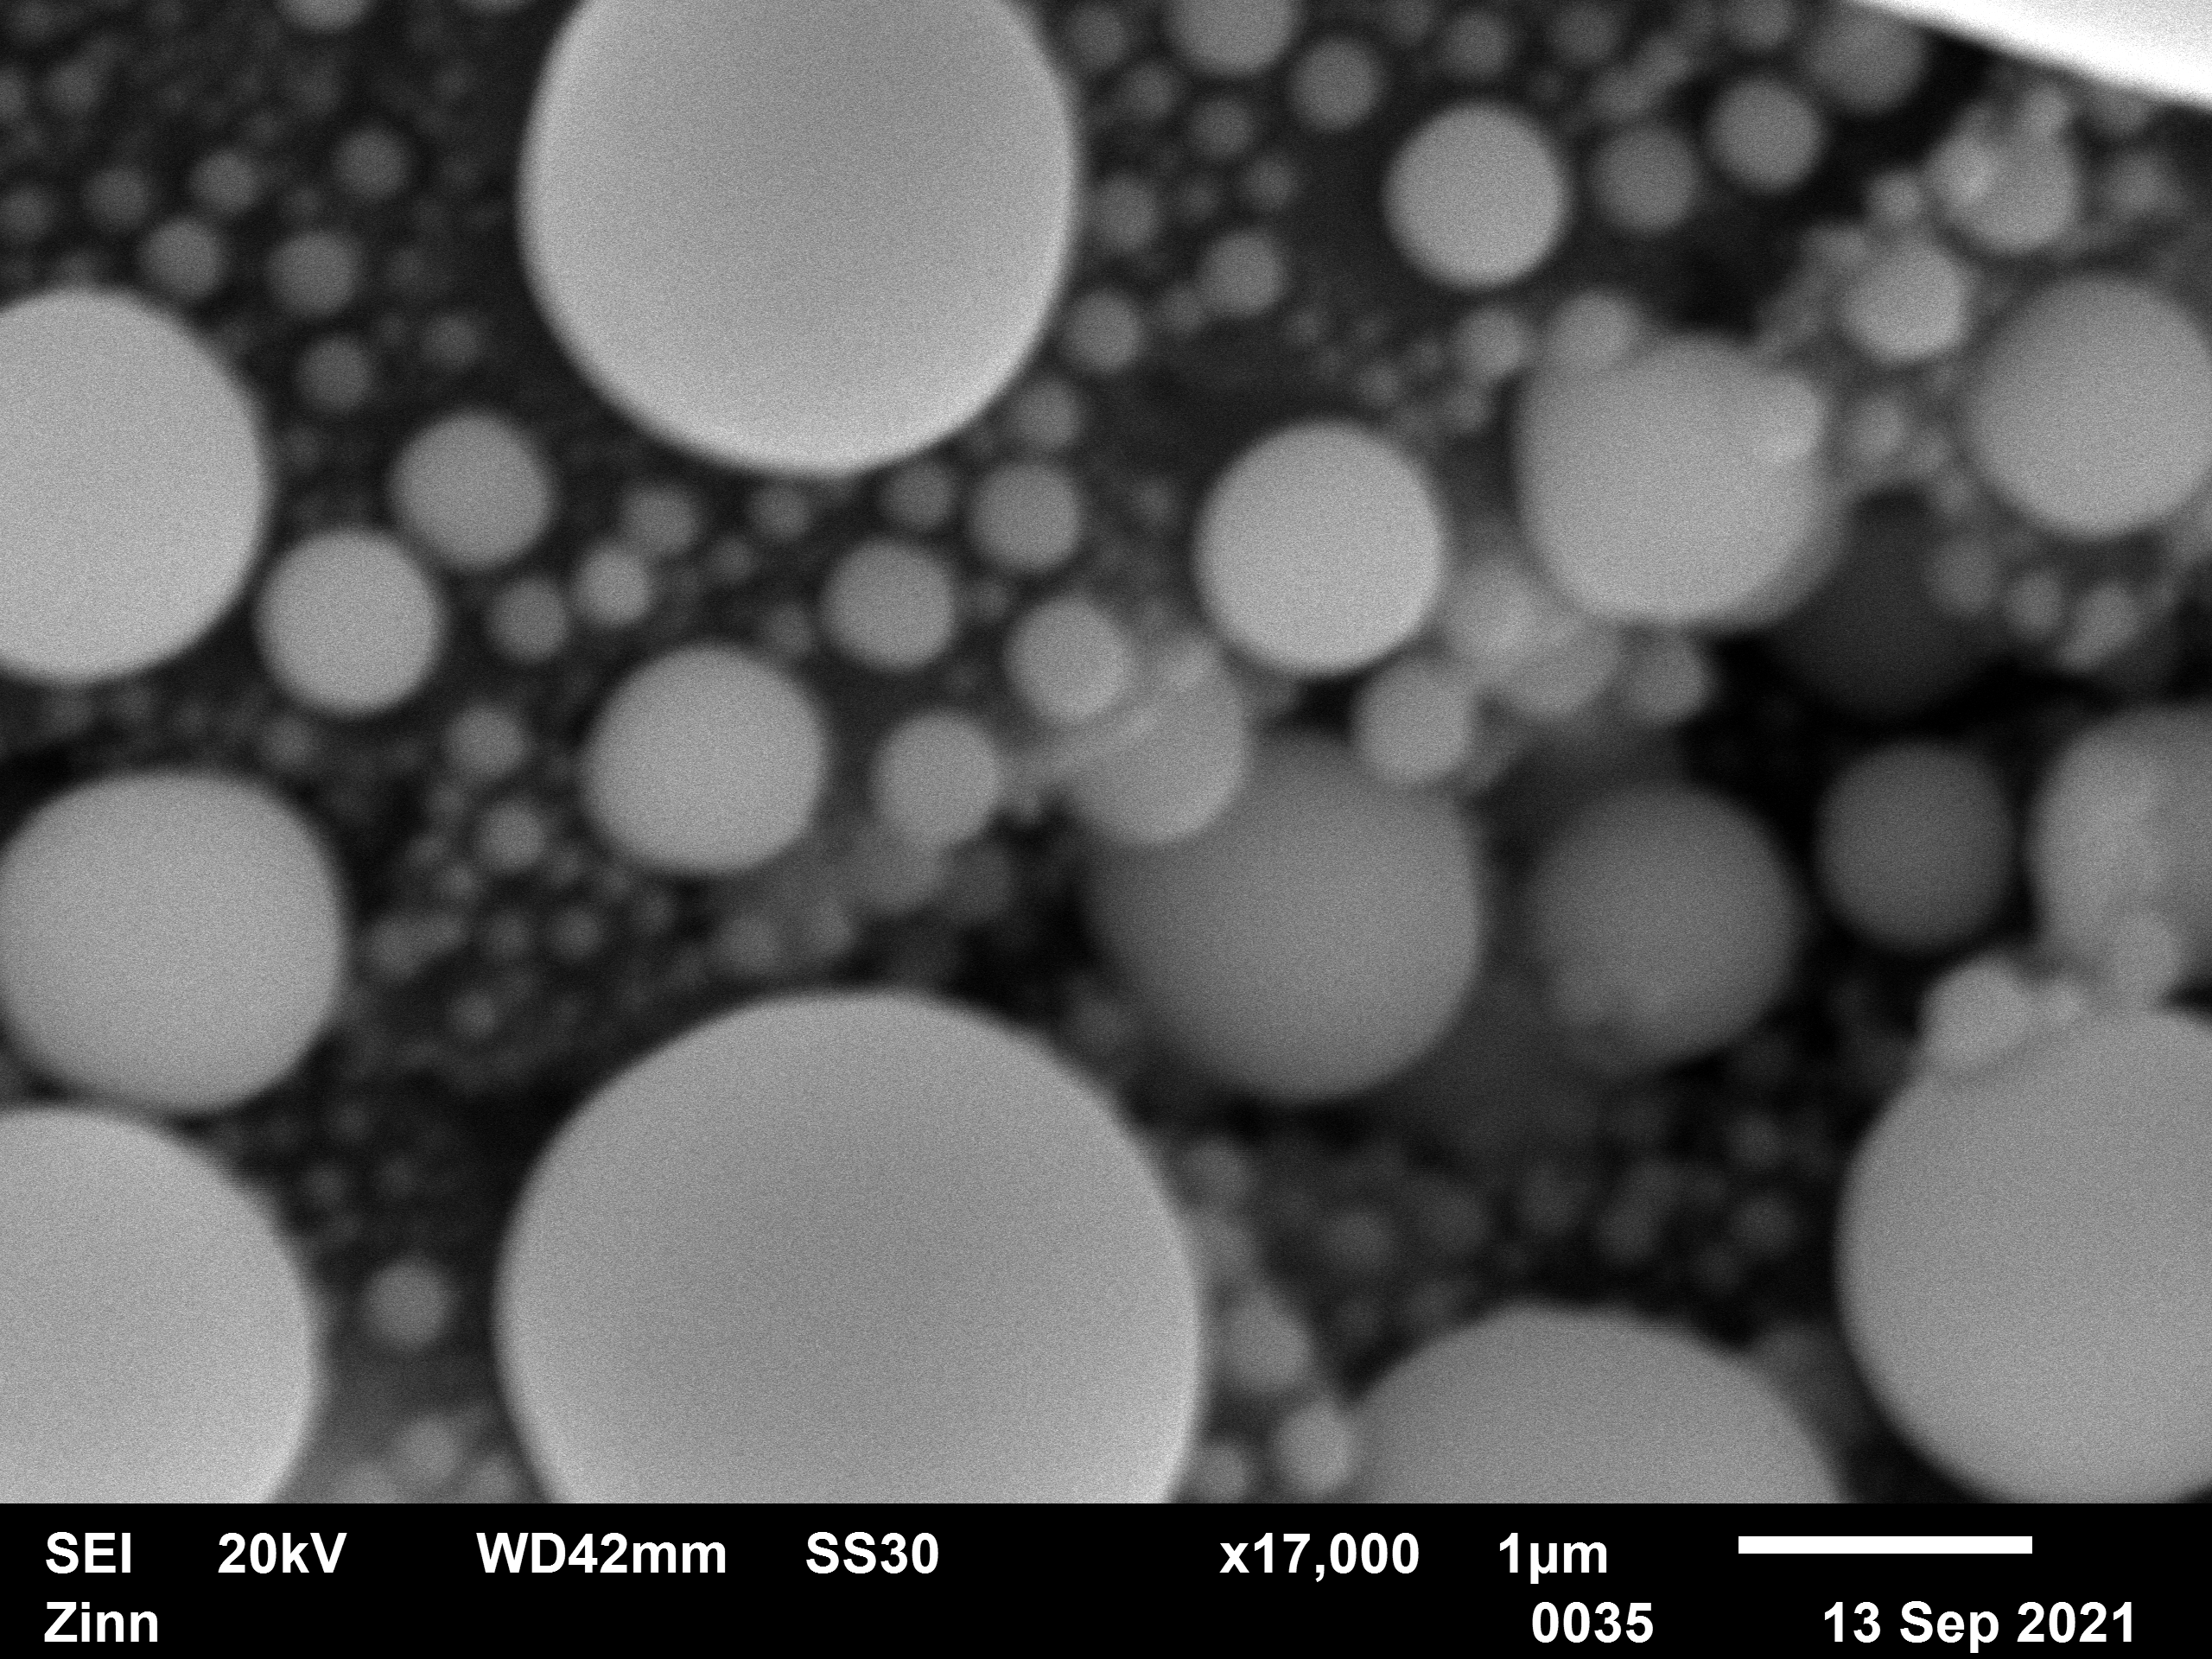
\includegraphics[width=\textwidth]{Auswertung/C/0035.png}
        \caption{SS 30}
    \end{subfigure}
    \hfill
    \begin{subfigure}[b]{0.25\textwidth}
        \centering
        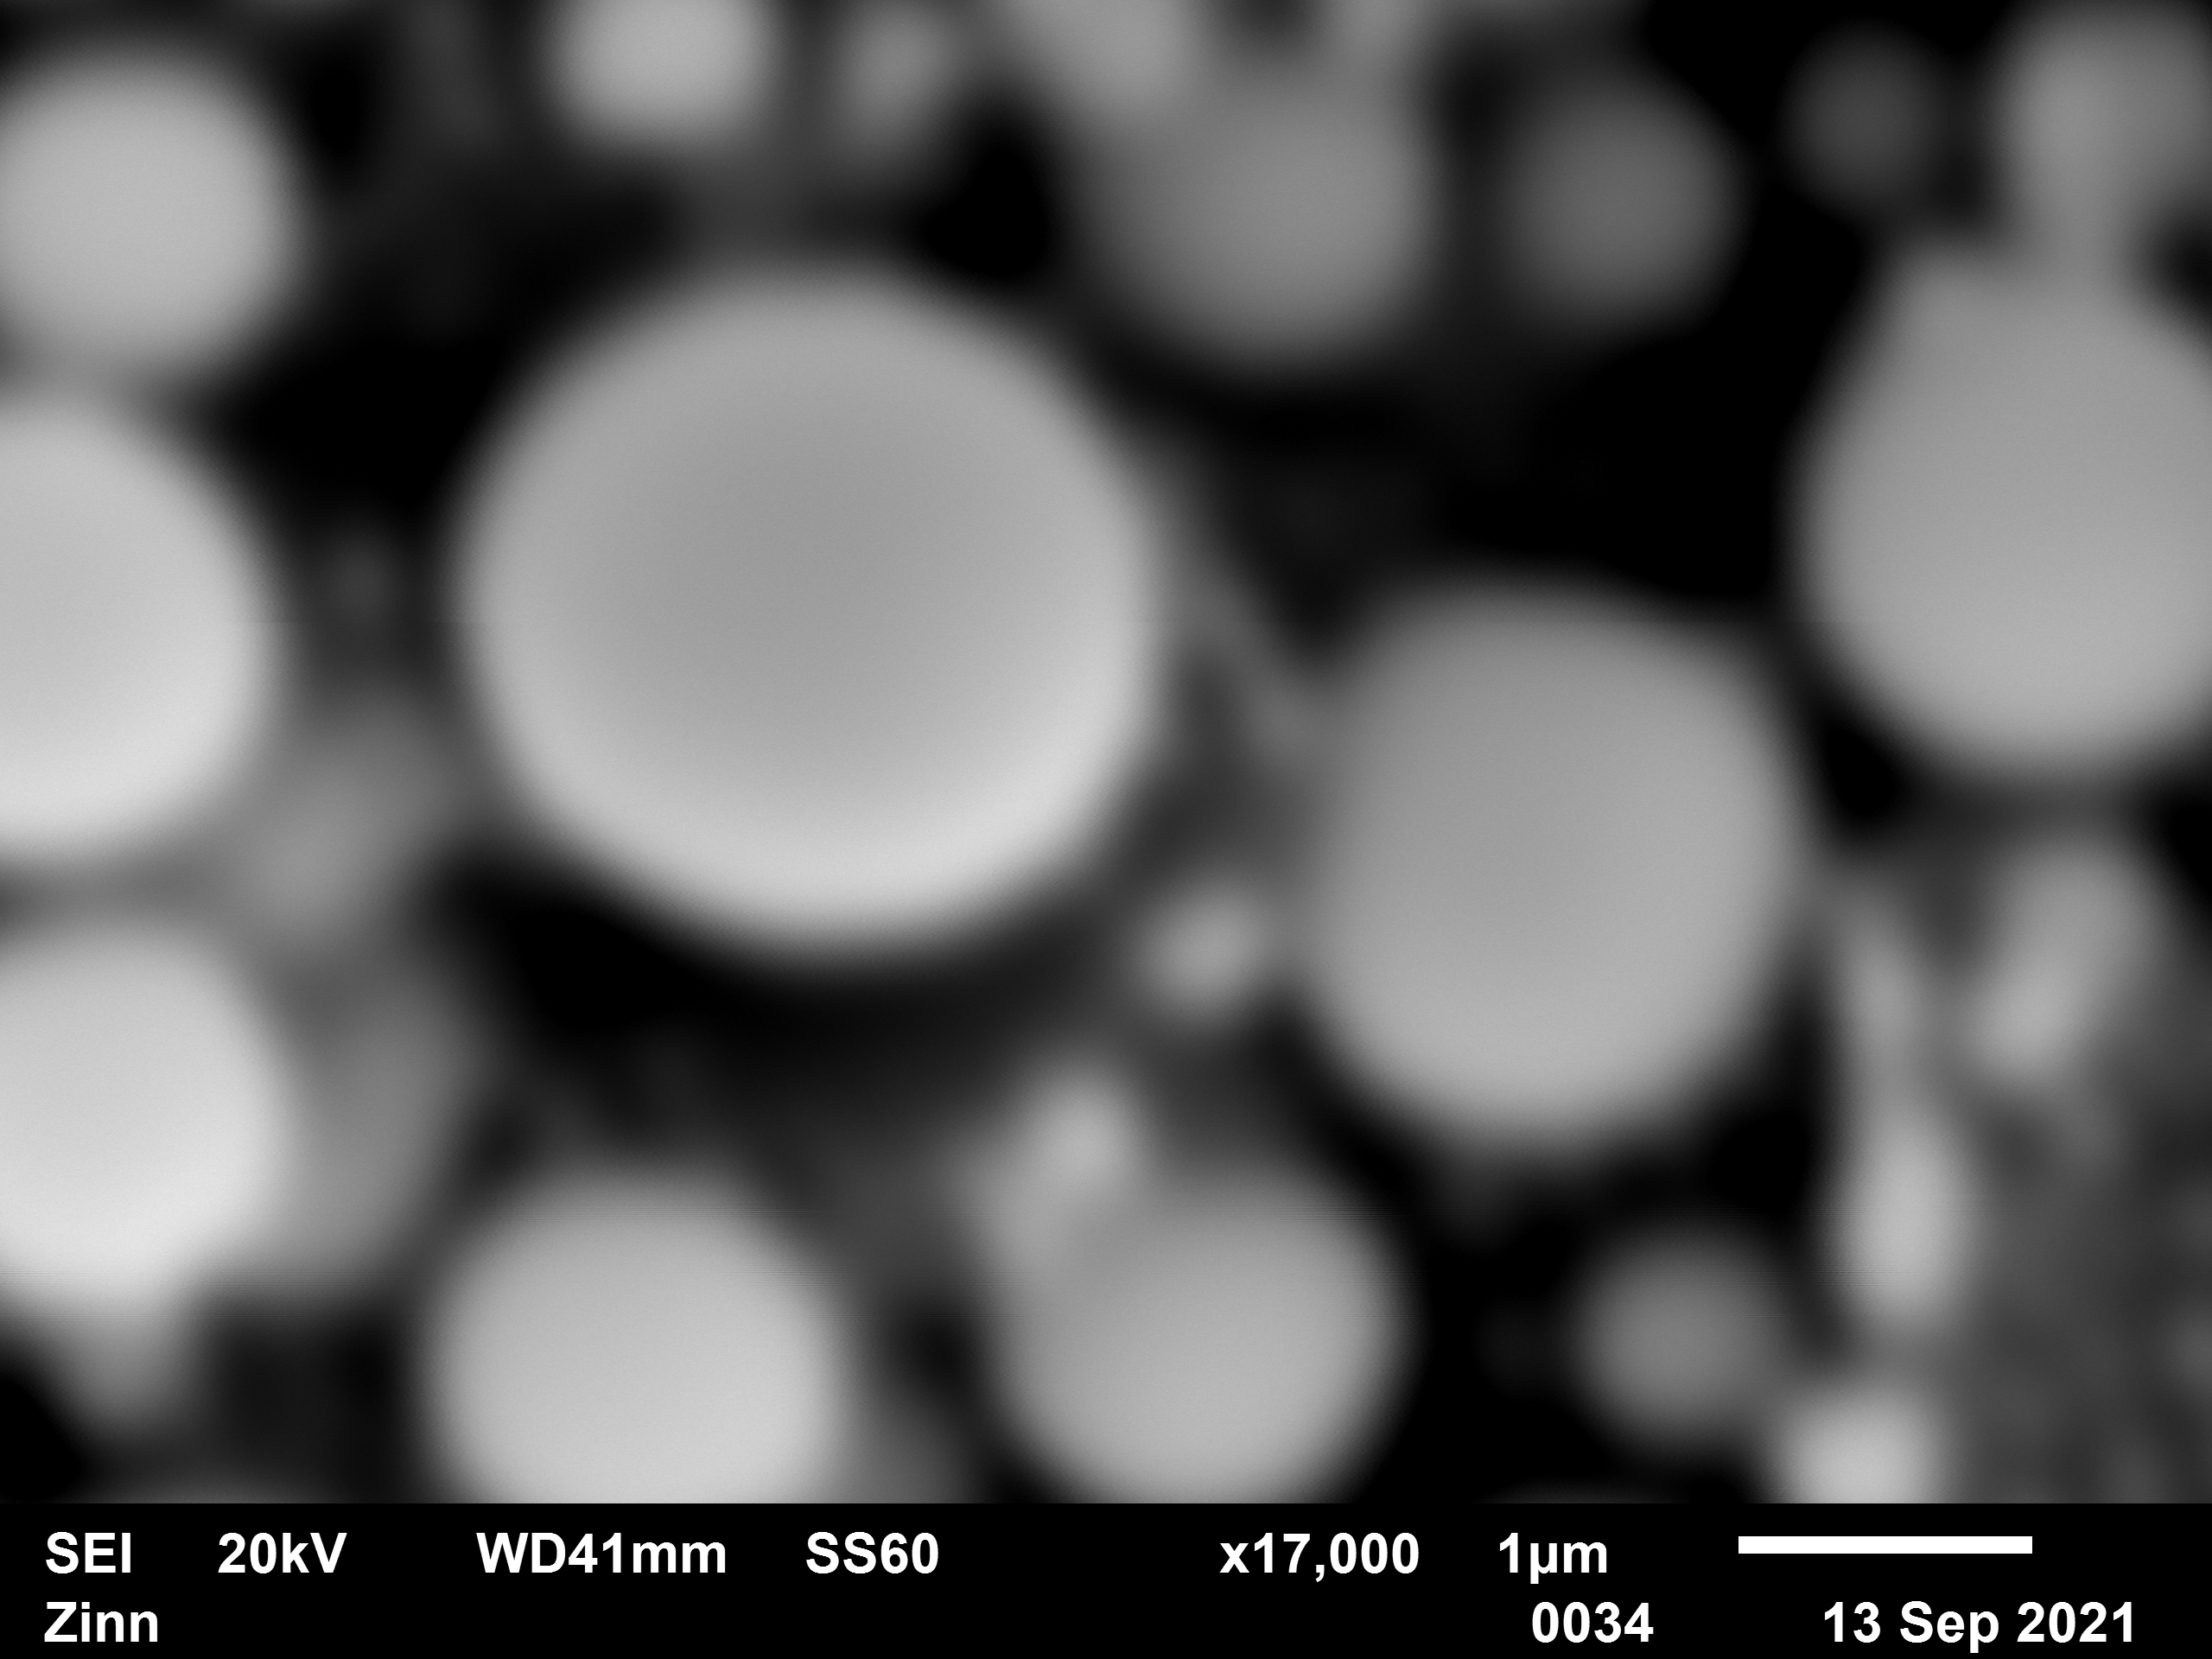
\includegraphics[width=\textwidth]{Auswertung/C/0034.png}
        \caption{SS 60}
    \end{subfigure}
    \caption{Zinstandart bei verschiedenen Strahldurchmessern}
\end{figure}

Es fällt auf, dass mit größerem SS die Schärfe und die Auflösung der Aufnahmen Schlechter wurden.

Außerdem wird auch die Beschleunigungsspannung variiert.
\begin{figure}[h]
    \centering
    \begin{subfigure}[b]{0.25\textwidth}
        \centering
        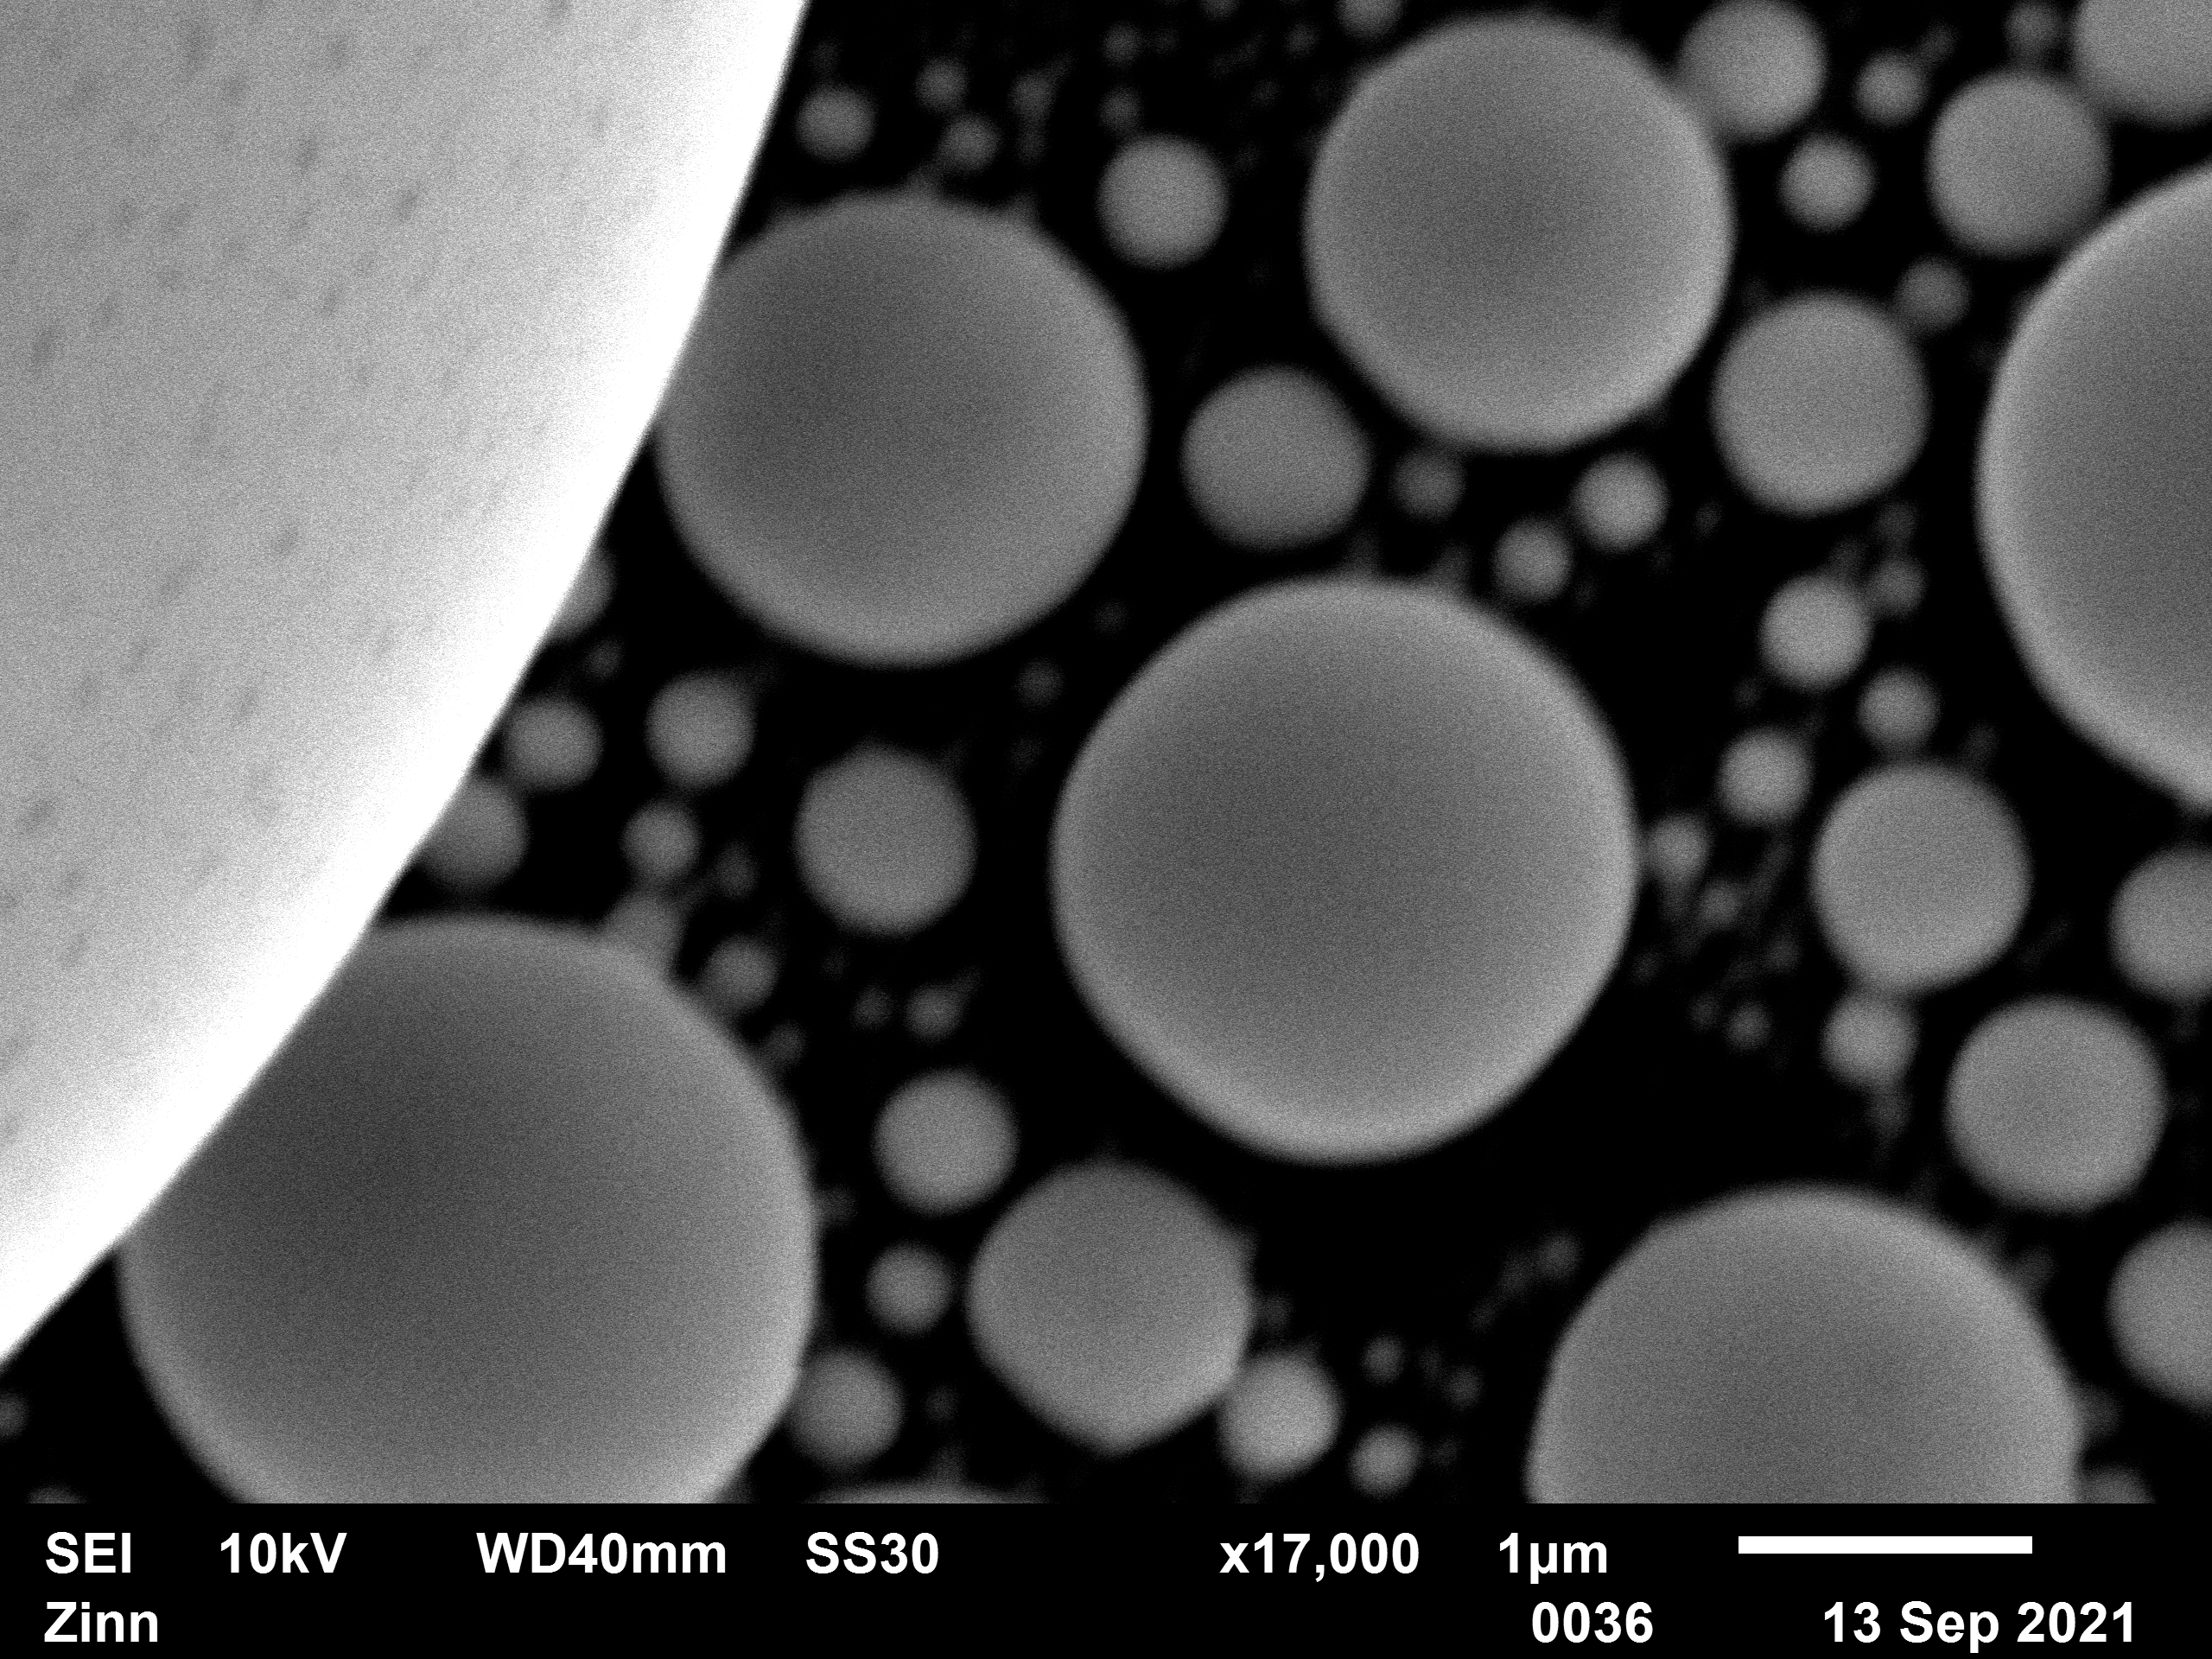
\includegraphics[width=\textwidth]{Auswertung/C/0036.png}
        \caption{10 kV}
    \end{subfigure}
    \hfill
    \begin{subfigure}[b]{0.25\textwidth}
        \centering
        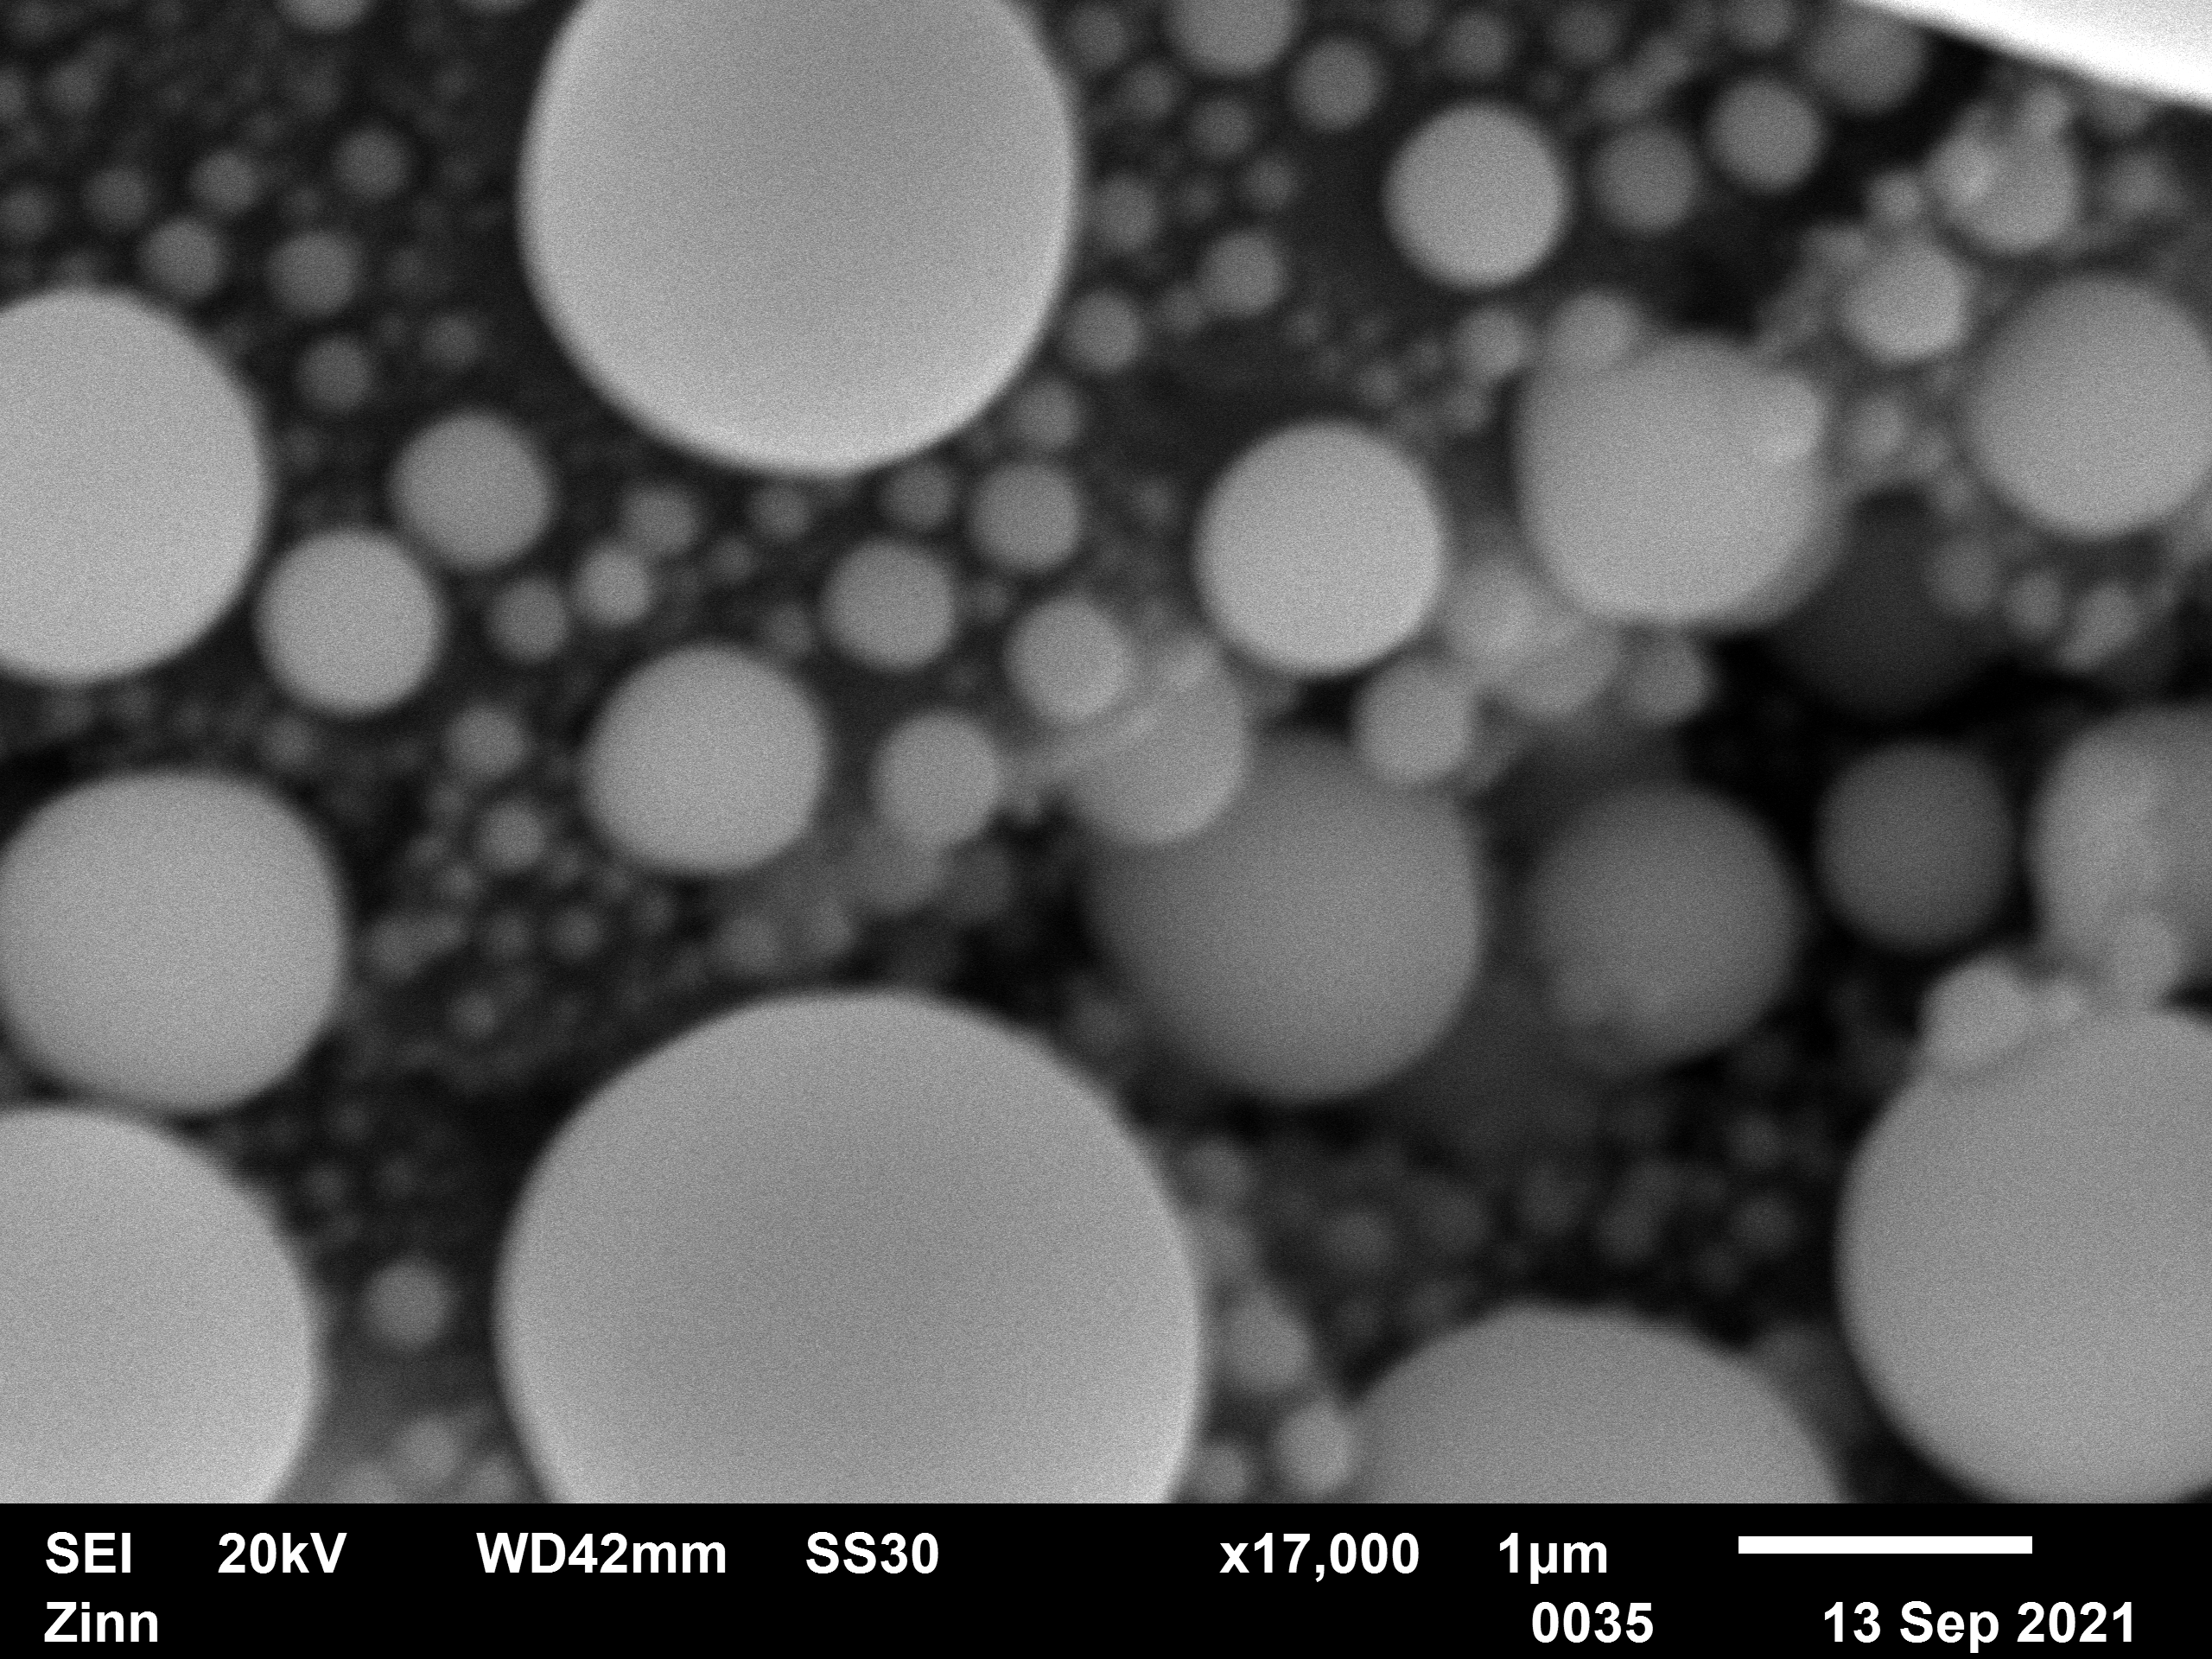
\includegraphics[width=\textwidth]{Auswertung/C/0035.png}
        \caption{20 kV}
    \end{subfigure}
    \hfill
    \begin{subfigure}[b]{0.25\textwidth}
        \centering
        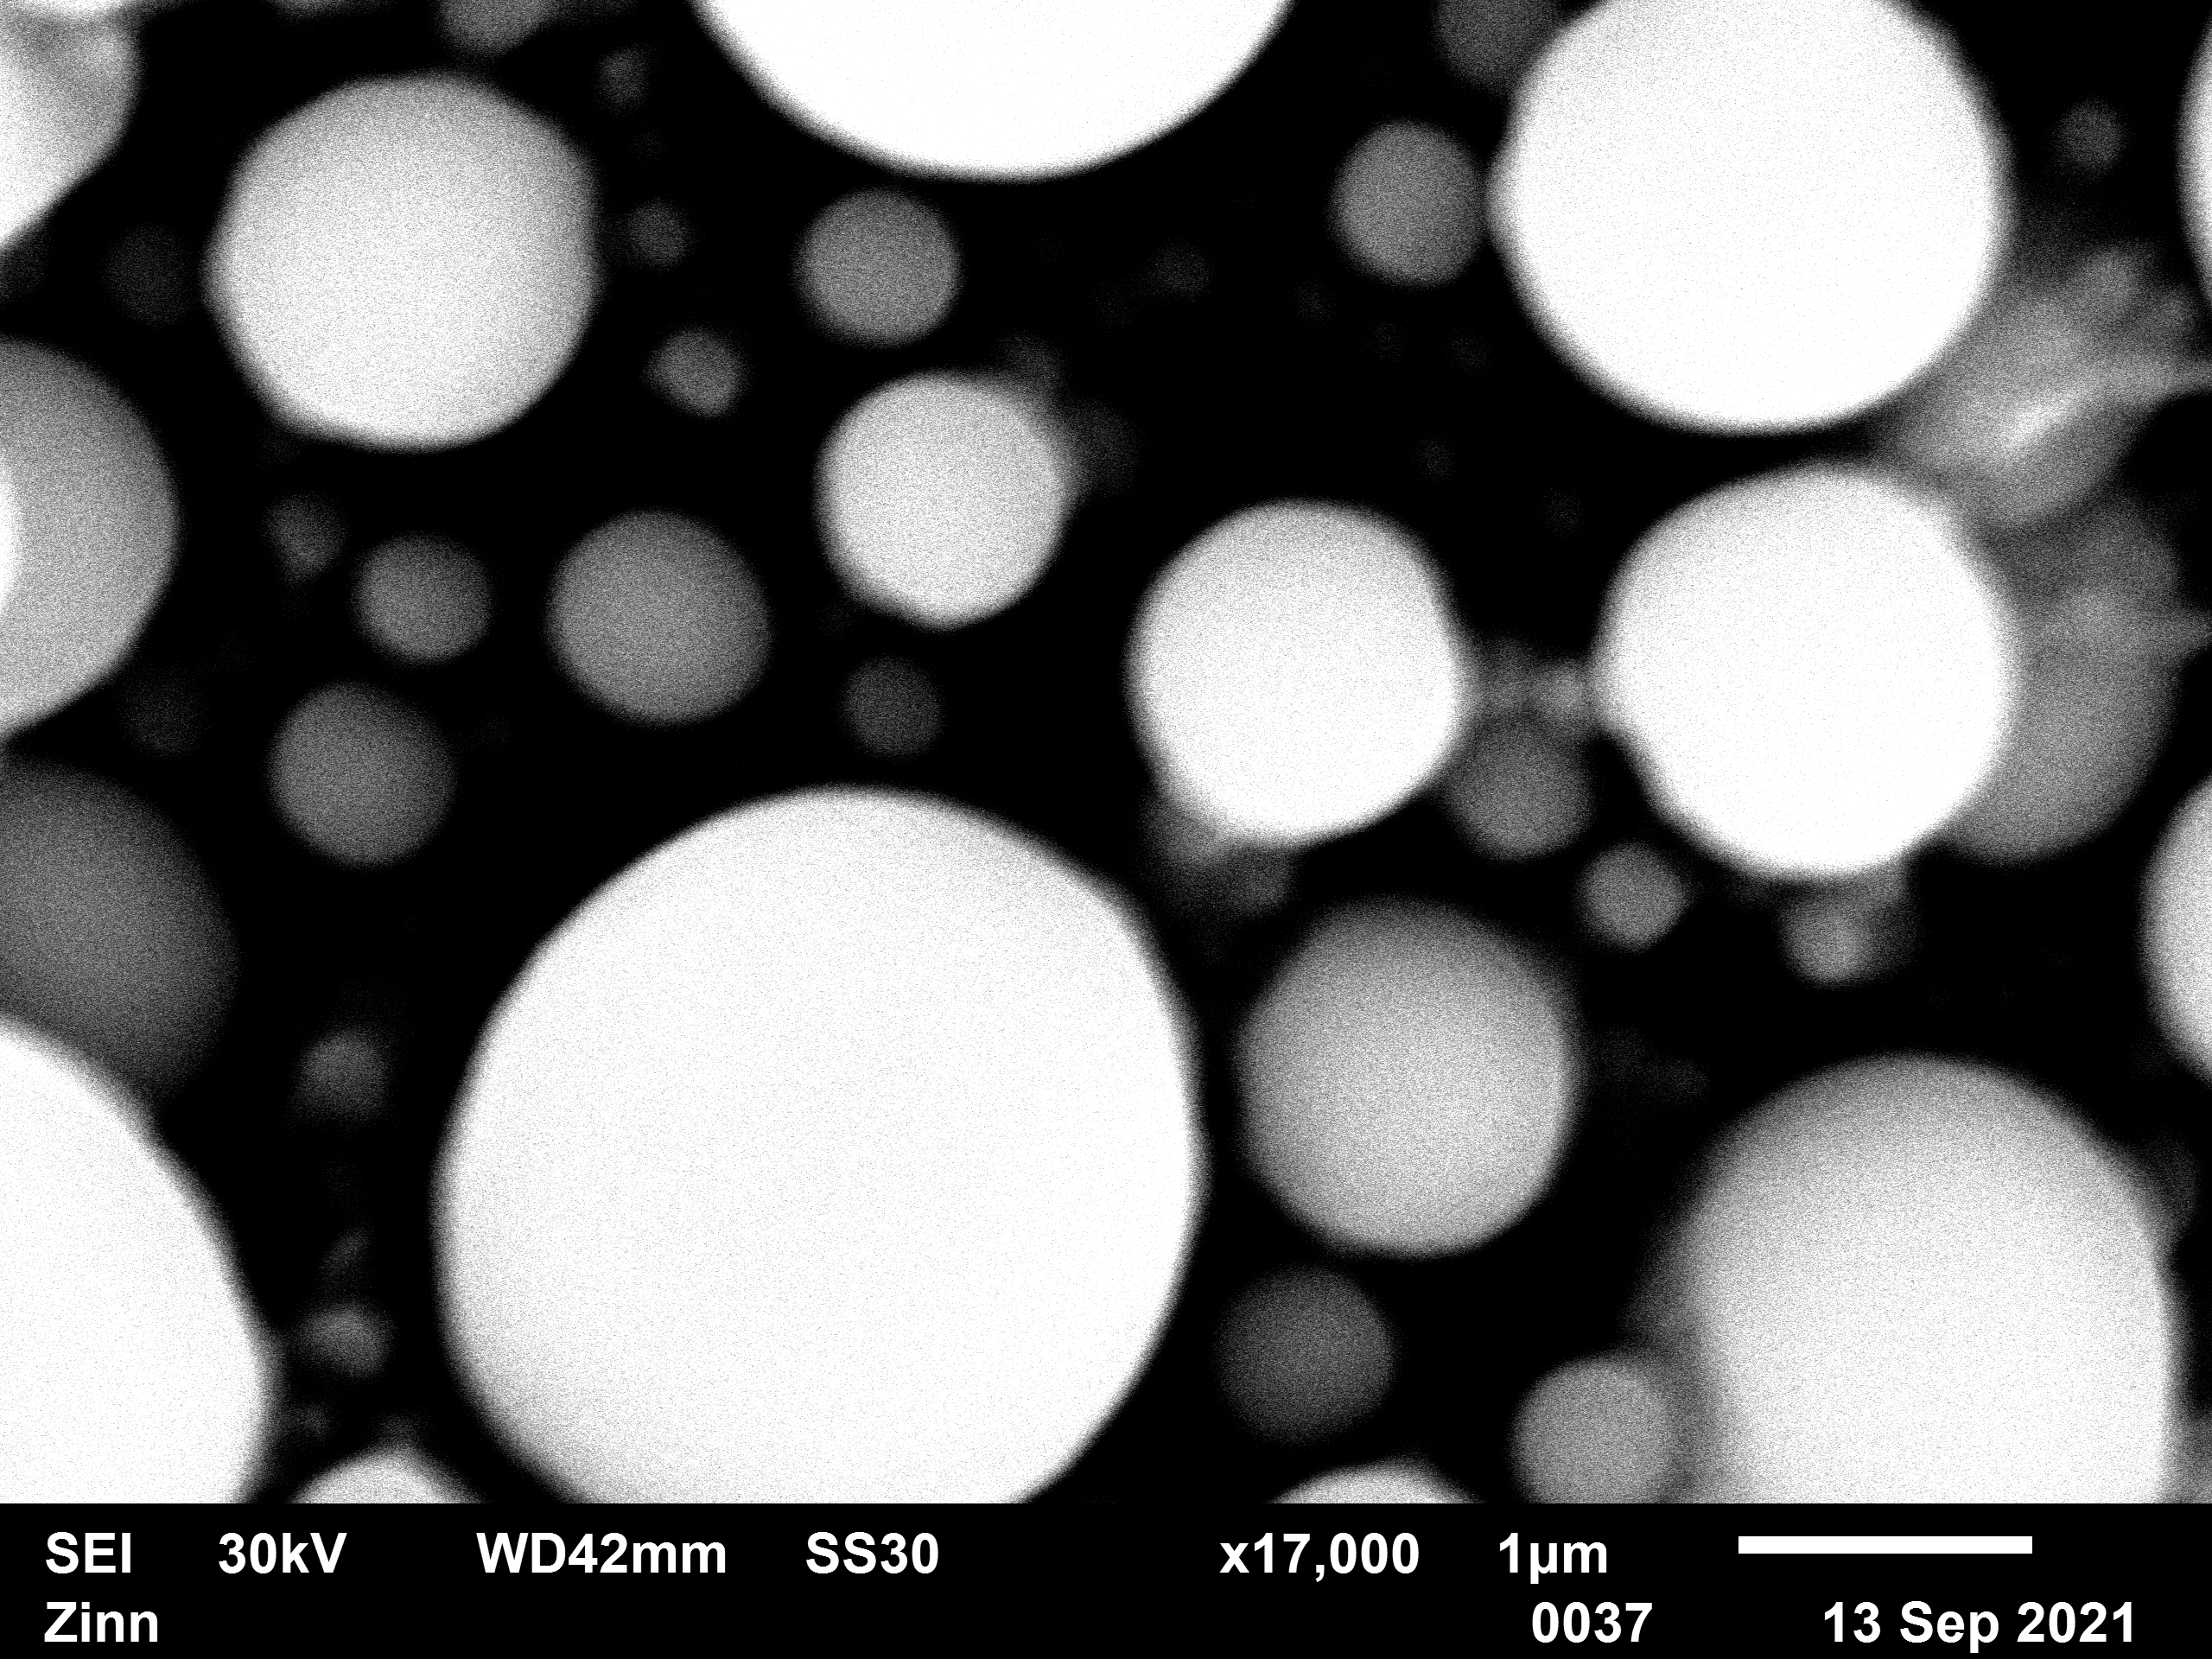
\includegraphics[width=\textwidth]{Auswertung/C/0037.png}
        \caption{30 kV}
    \end{subfigure}
    \caption{Zinstandart bei verschiedenen Beschleunigunsspannungen}
\end{figure}

Es fällt auf, dass bei 20 kV sehr viele Kugeln im hintergrund zu erkennen sind, wohingegen dies bei 30 kV fast gar nicht mehr der Fall ist. Es scheint nicht so als würde die Beschleunigungsspannung nier einen konkreten Unterschied bewirken, da keine klare Tendenz zu erkennen ist.

\newpage
Zum Schluss wurde dann der Arbeitsabstand variiert.
\begin{figure}[h]
    \centering
    
    \begin{subfigure}[b]{0.45\textwidth}
        \centering
        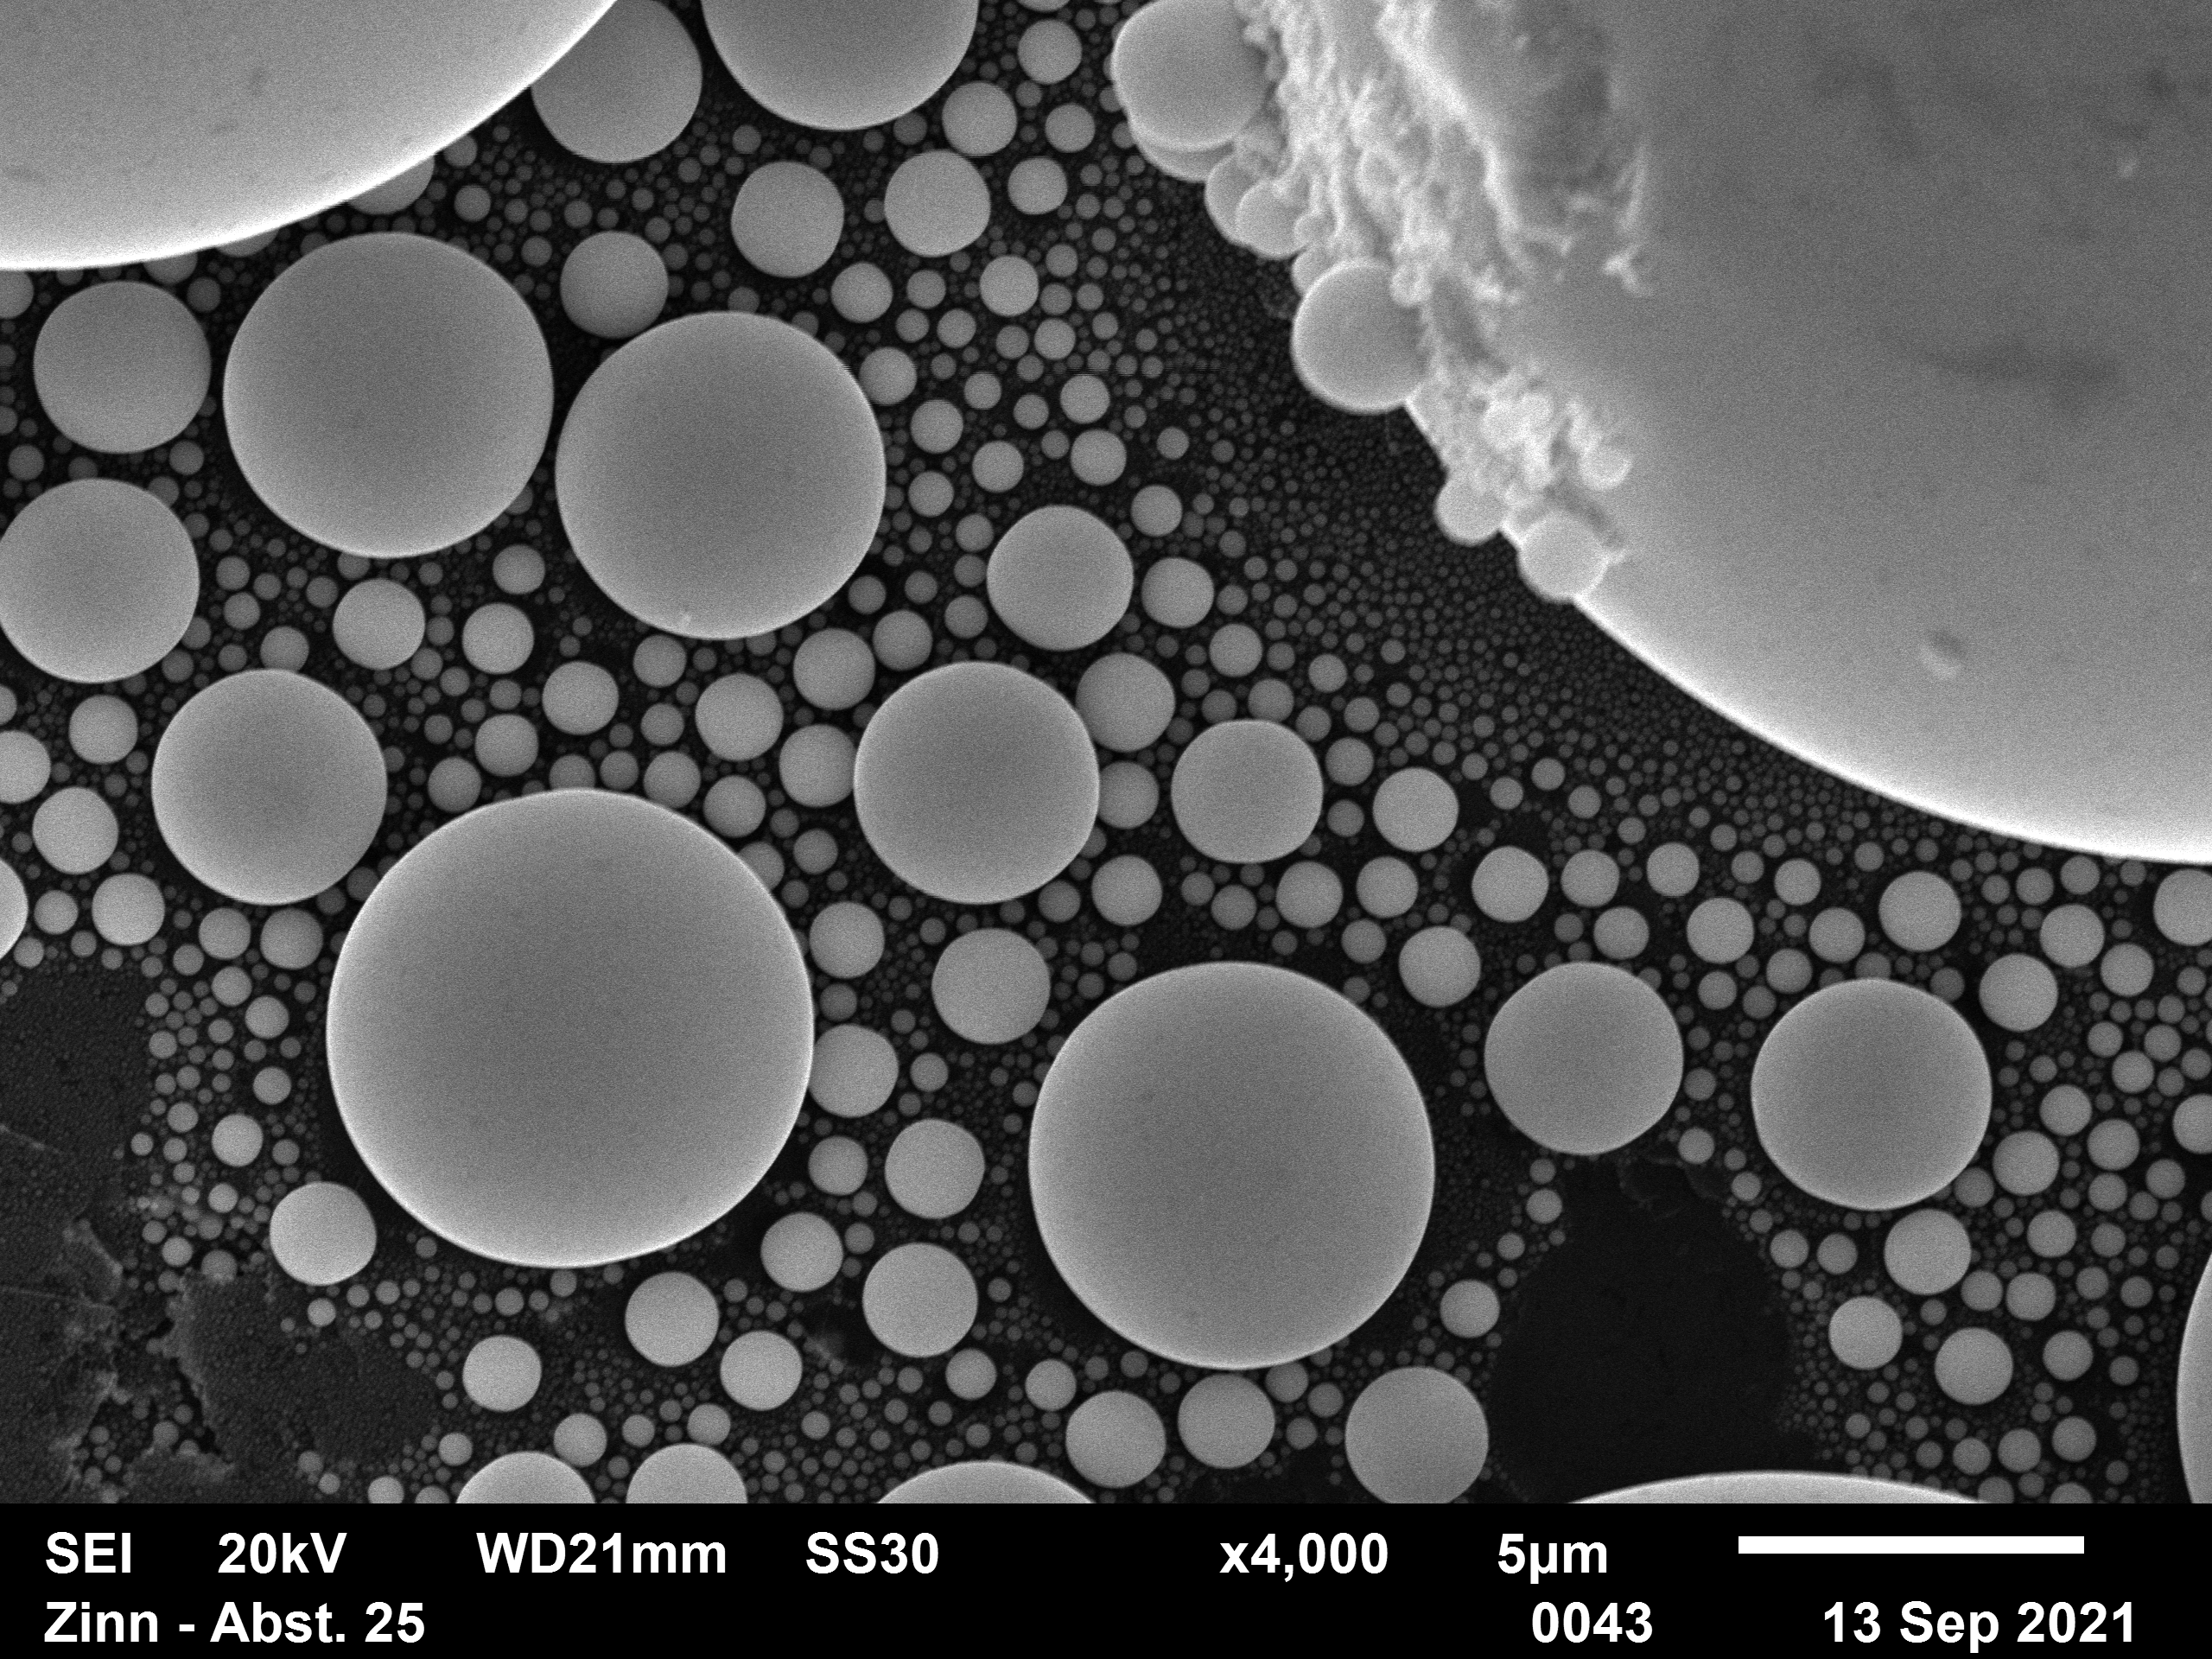
\includegraphics[width=\textwidth]{Auswertung/C/0043.png}
        \caption{Arbeitsabstand 25 mm}
    \end{subfigure}
    \hfill
    \begin{subfigure}[b]{0.45\textwidth}
        \centering
        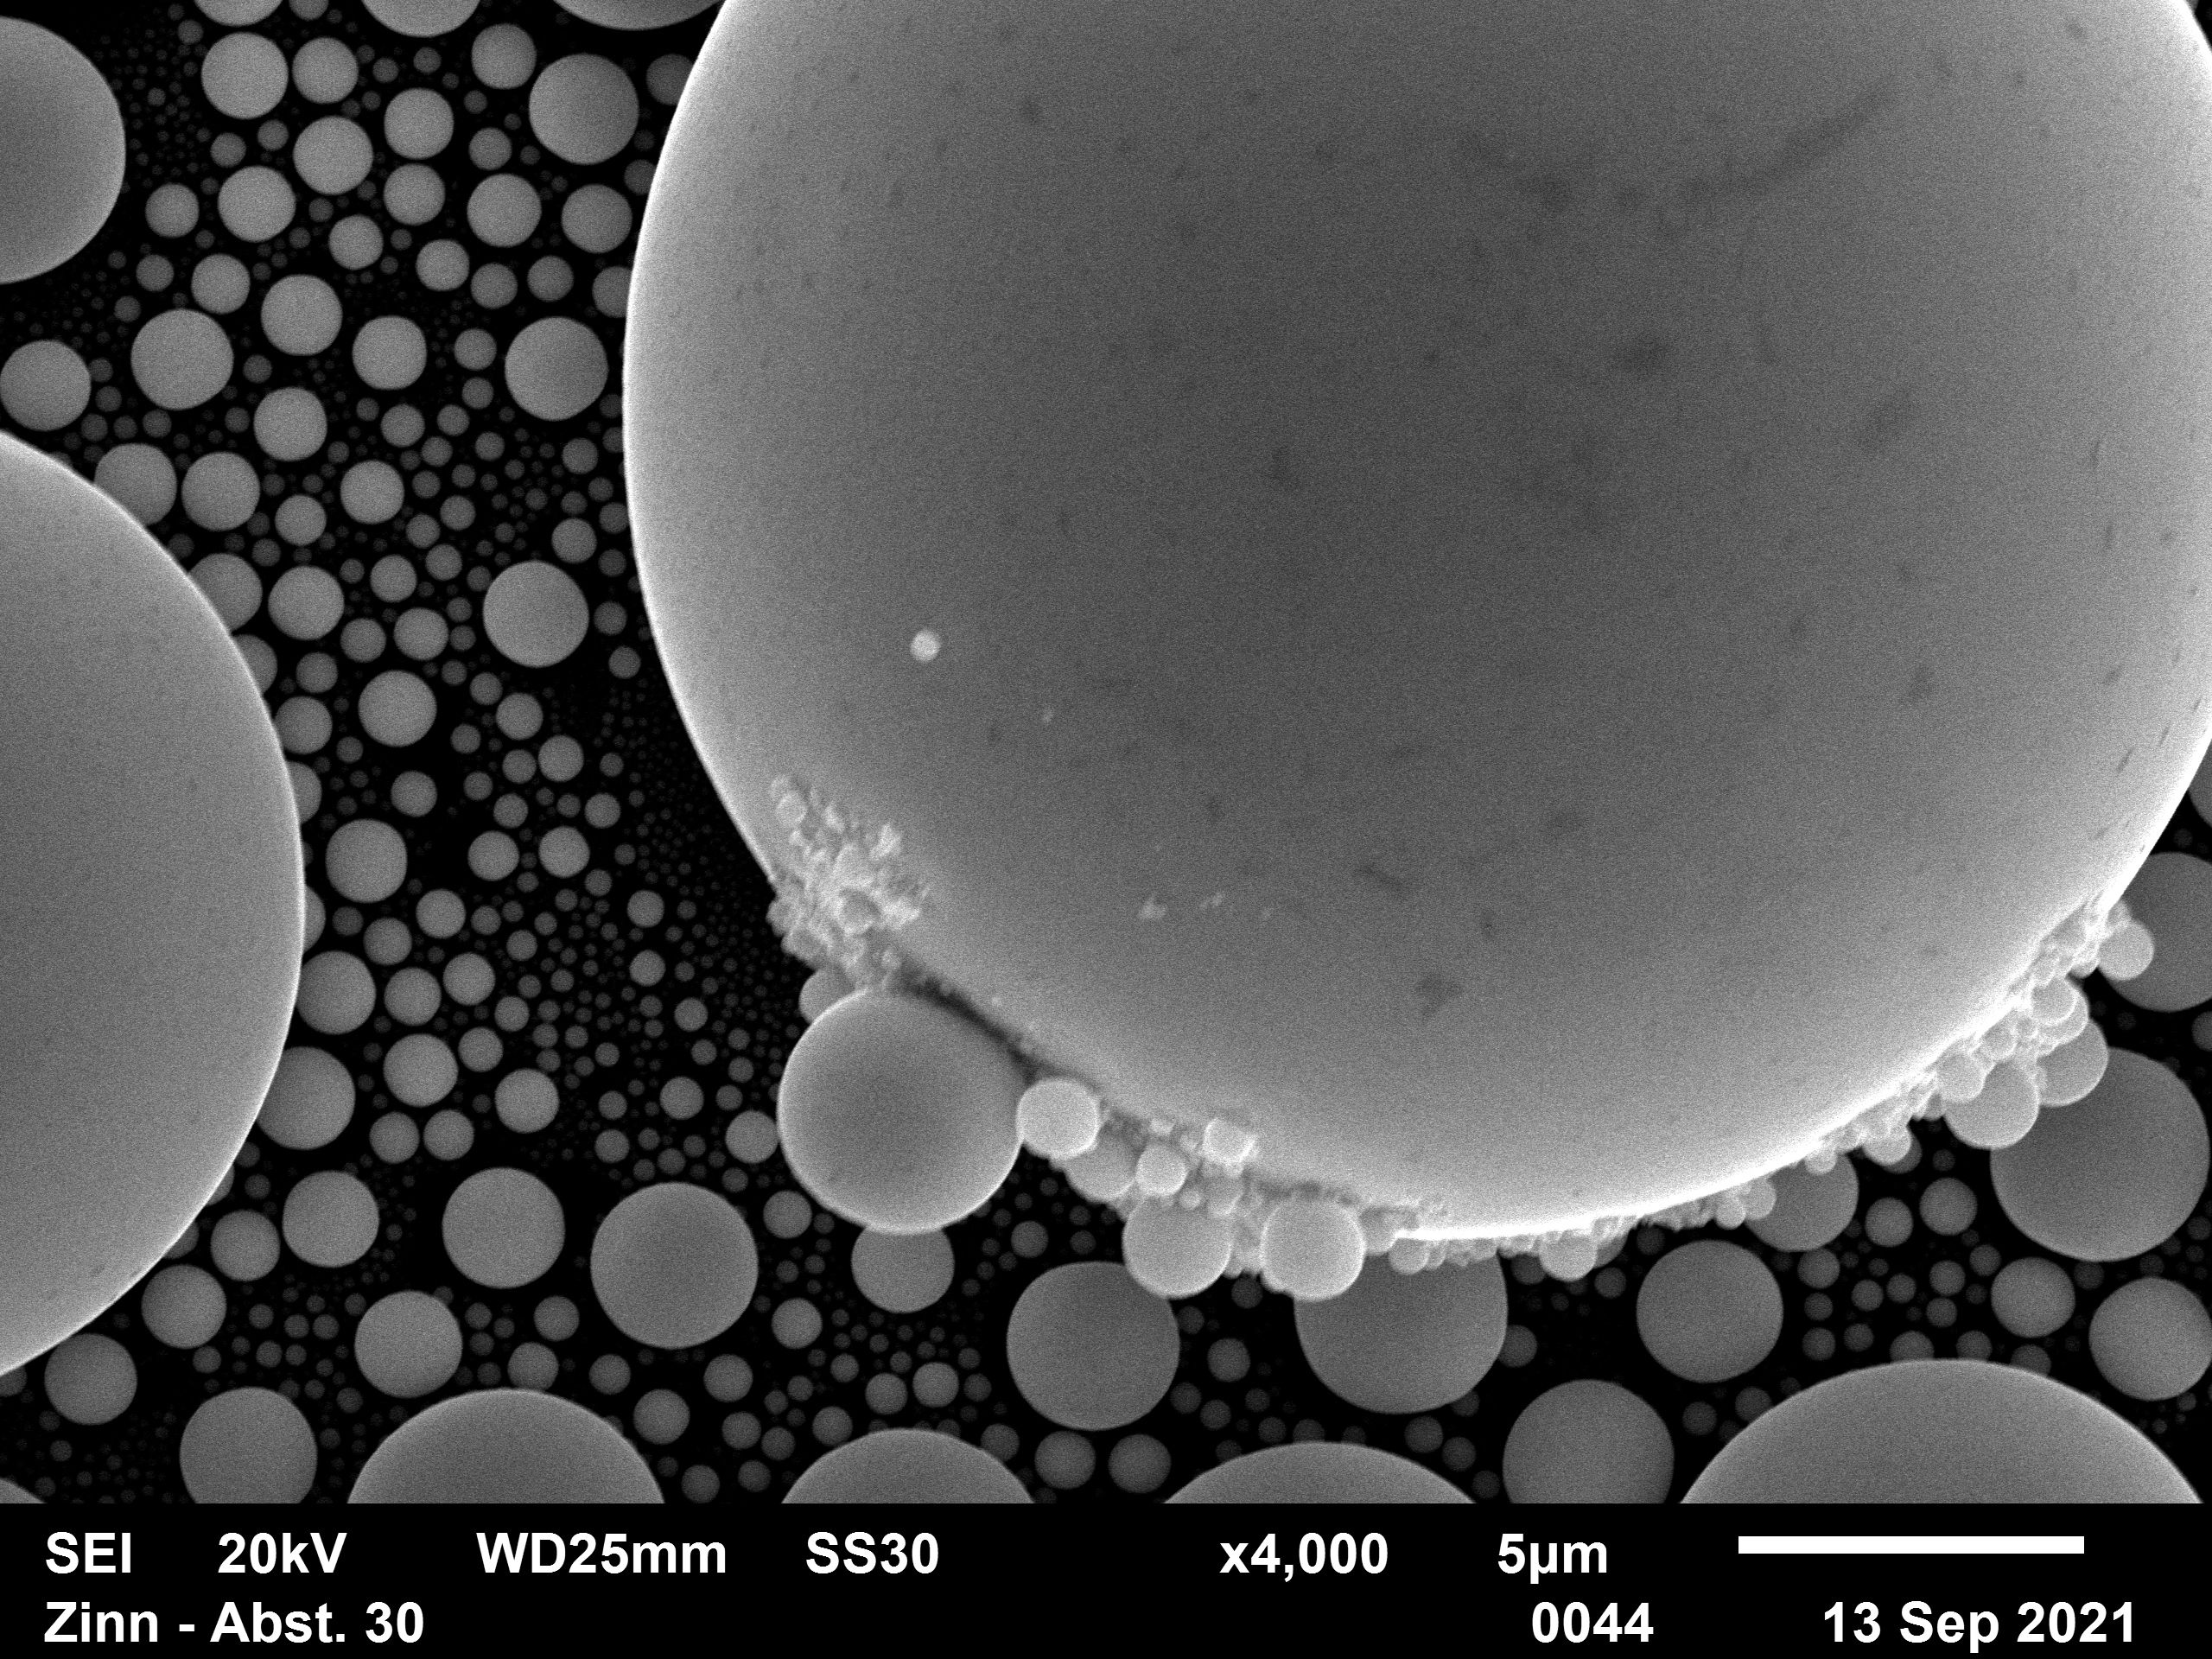
\includegraphics[width=\textwidth]{Auswertung/C/0044.png}
        \caption{Arbeitsabstand 30 mm}
    \end{subfigure}
    
    \caption{Zinnstandartbei unterschiedlichen Arbeitsabstand}
\end{figure}

Im bezug auf den Arbeitsabstand fällt auf, dass mit dessen Verringerung mehrere kleinere Kugeln in den hinteren ebenen zu erkennen sind.

\newpage
\section{Gebrochene Schraube}

In folgenden Versuchsteil soll die Bruchuhrsache einer Schraube ermittelt werden.

Im ersten Schritt wurden hierzu Bilder der Bruchfläche mit verschiedenen Detektoren aufgenommen.
\begin{figure}[h]
    \centering
    
    \begin{subfigure}[b]{0.45\textwidth}
        \centering
        \includegraphics[width=\textwidth]{Auswertung/D/0049.png}
        \caption{SEI}
    \end{subfigure}
    \hfill
    \begin{subfigure}[b]{0.45\textwidth}
        \centering
        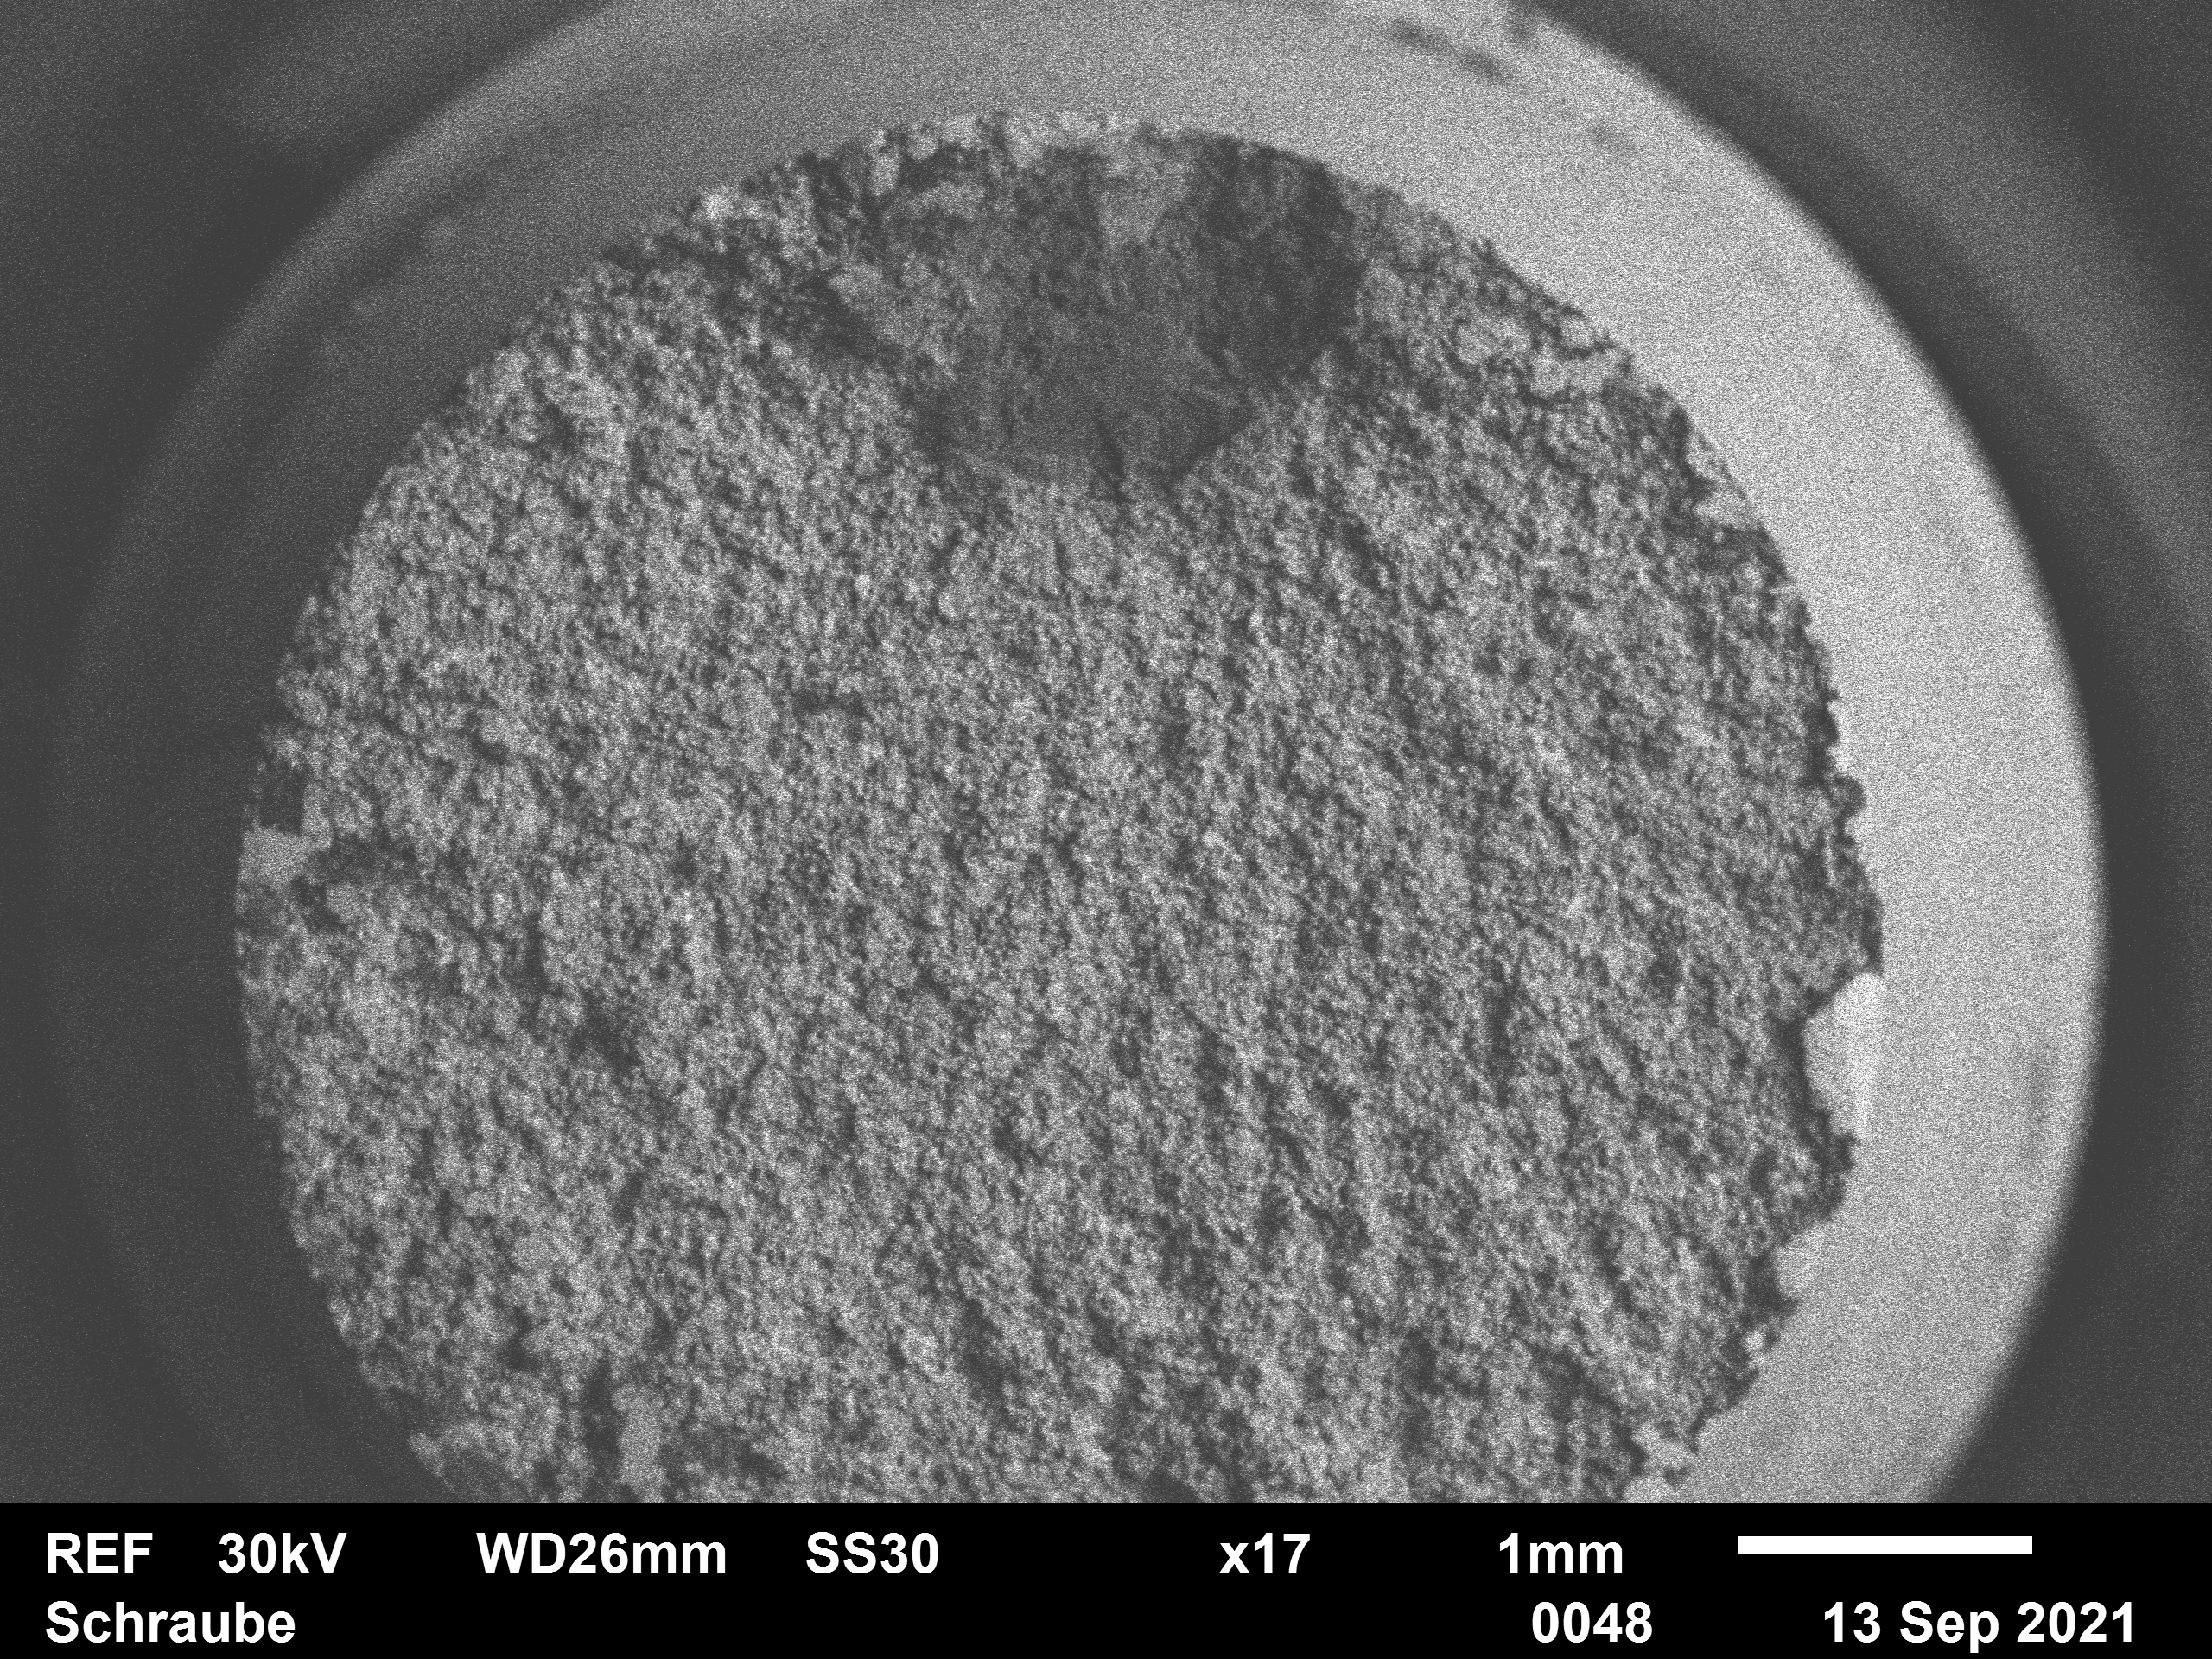
\includegraphics[width=\textwidth]{Auswertung/D/0048.png}
        \caption{REF}
    \end{subfigure}
    \\
    \begin{subfigure}[b]{0.45\textwidth}
        \centering
        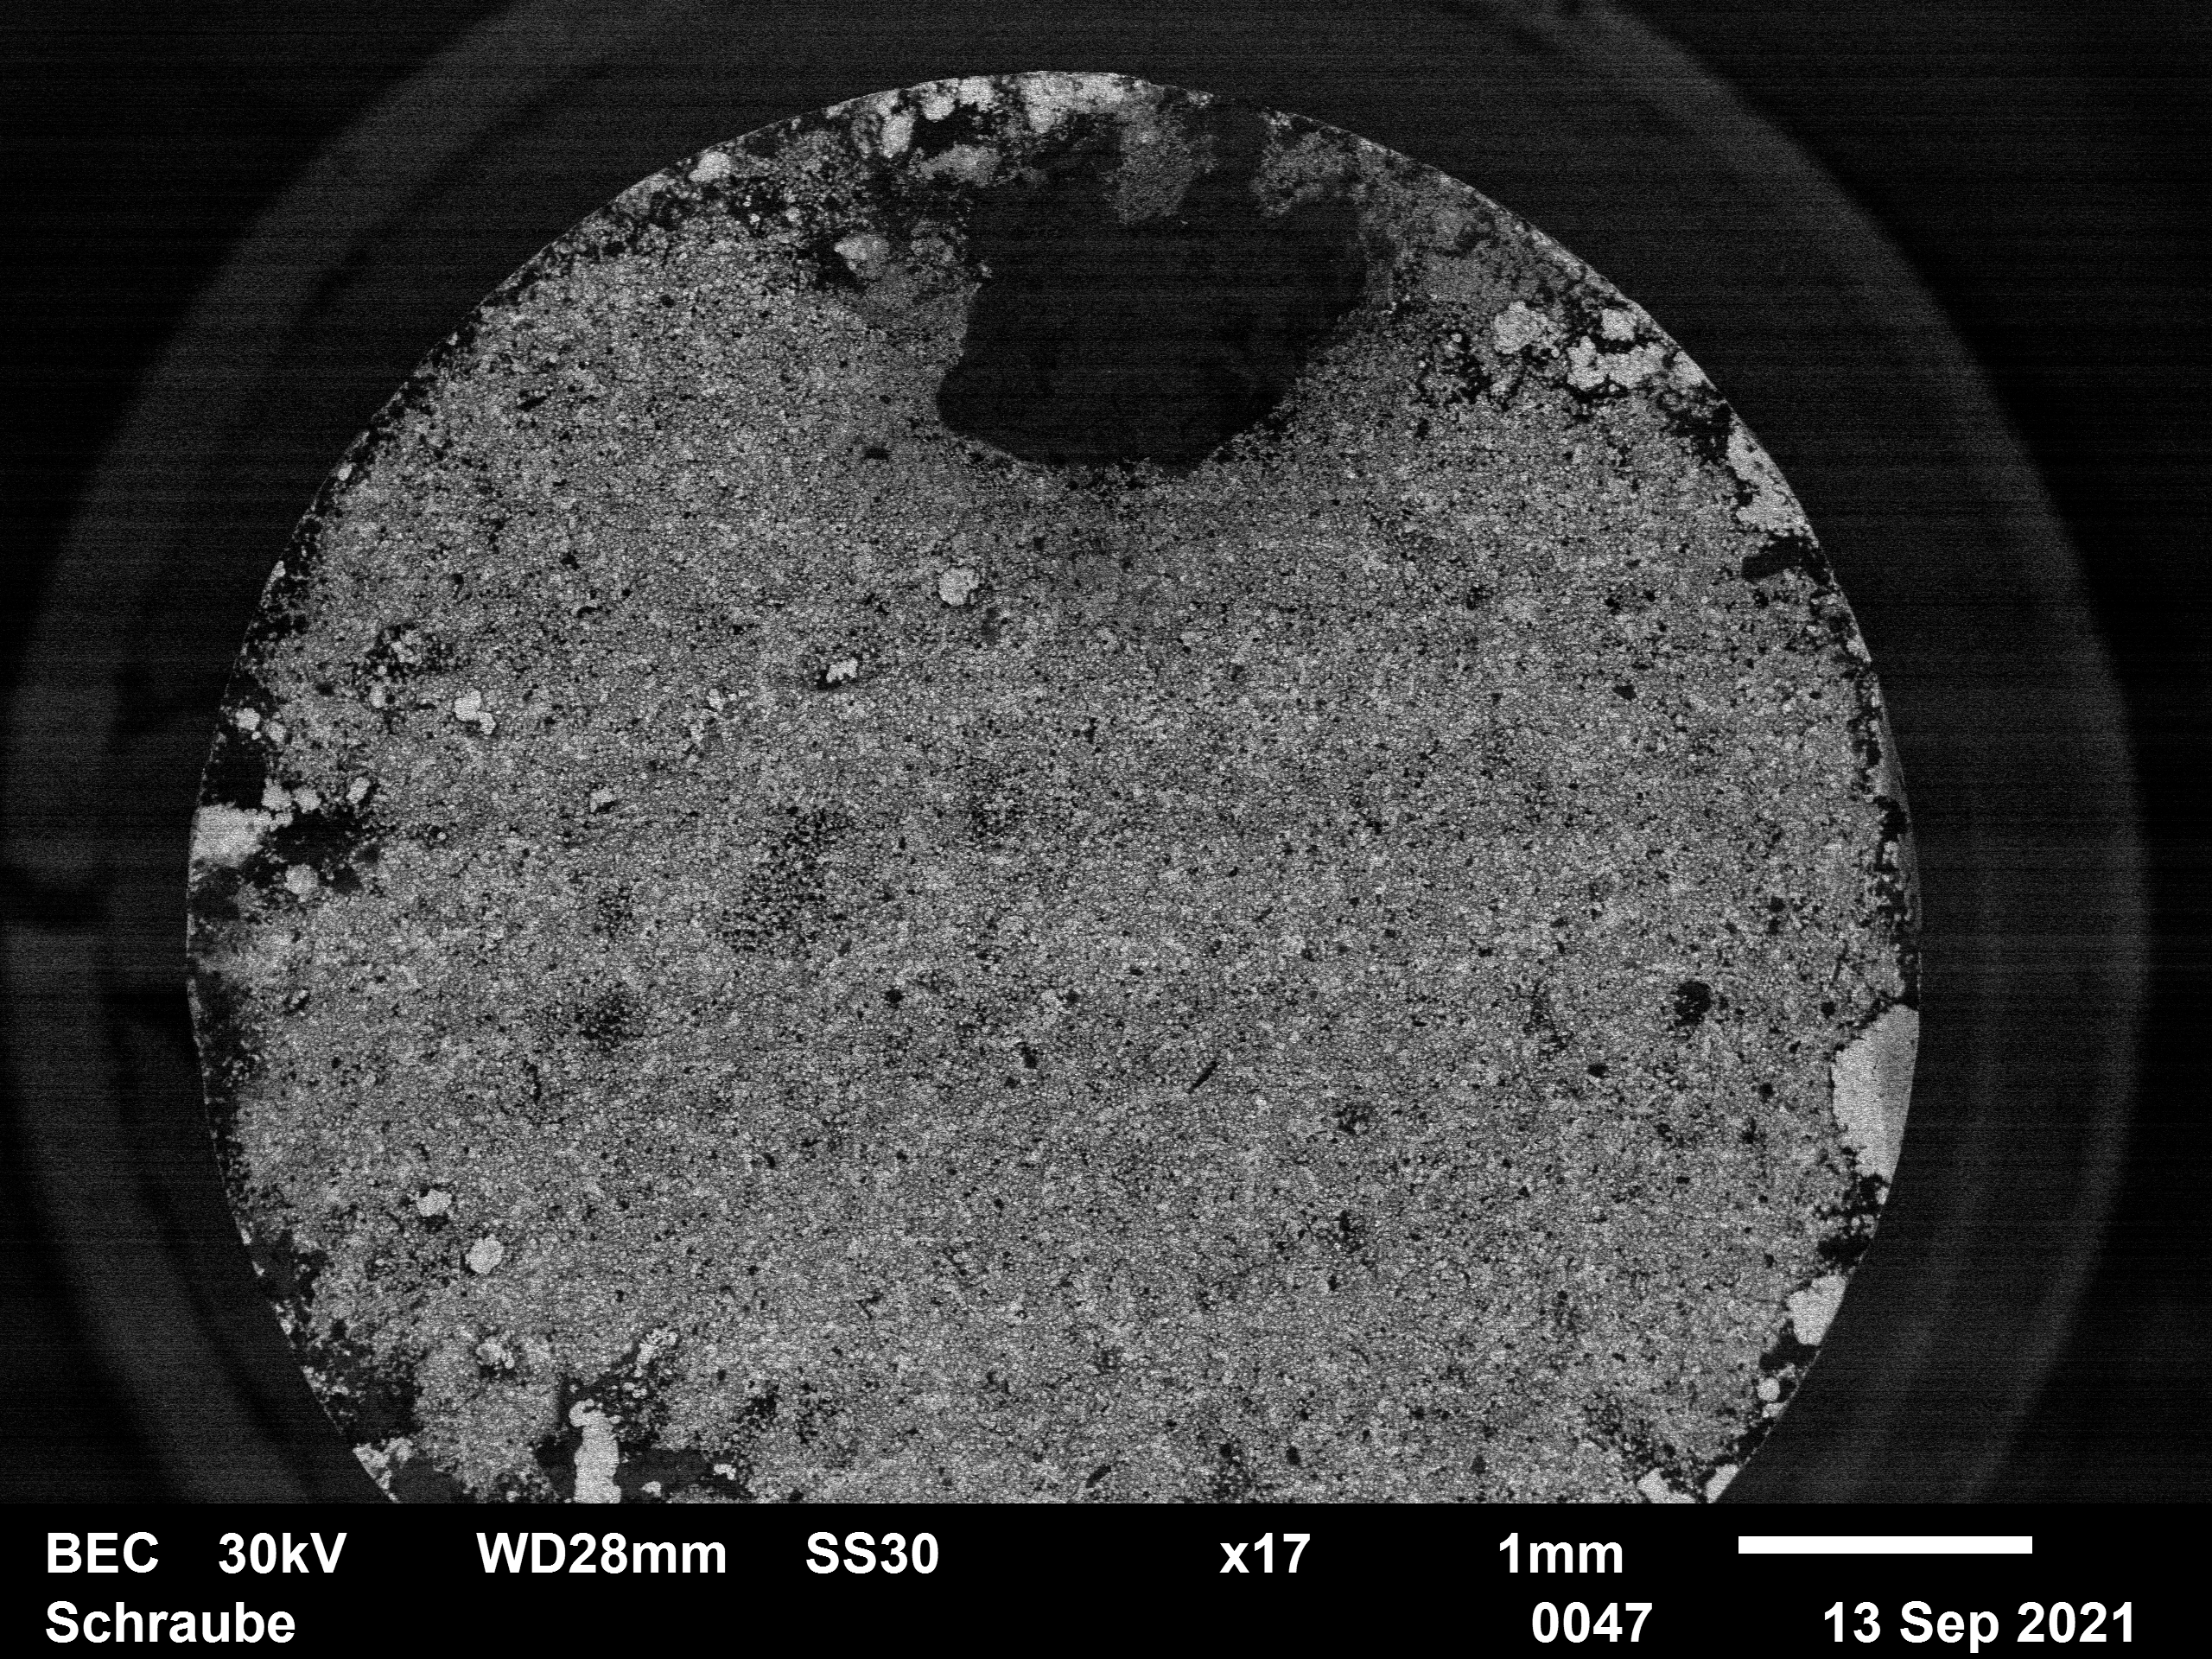
\includegraphics[width=\textwidth]{Auswertung/D/0047.png}
        \caption{BEC}
    \end{subfigure}
    \caption{Bruchfläche der Schraube mit unterschiedlichen Detektoren}
\end{figure}

Für einen guten ersten Eindruck eignet sich der SEI Modus, um die Struktur der Fläche zu untersuchen, eignet sich der REF Modus. In allen Aufnahmen und besonders im letzten Bild, im BEC Modus, sind drei unterschiedliche Zonen zu erkennen. Zum einen ein recht auffälliger dunkler Fleck im oberen Teil, daneben mehrere kleine hellere Zonen, die sich am Rand der Fläche zu konzentrieren scheinen und der übrige Teil der Schraube, dessen helligkeit zwischen den beiden anderen Zonen liegt. \\

\newpage
Als Nächstes wurde eine Nahaufnahme des dunklen Flecks angefertigt.
\begin{figure}[h]
    \centering
    
    \begin{subfigure}[b]{0.45\textwidth}
        \centering
        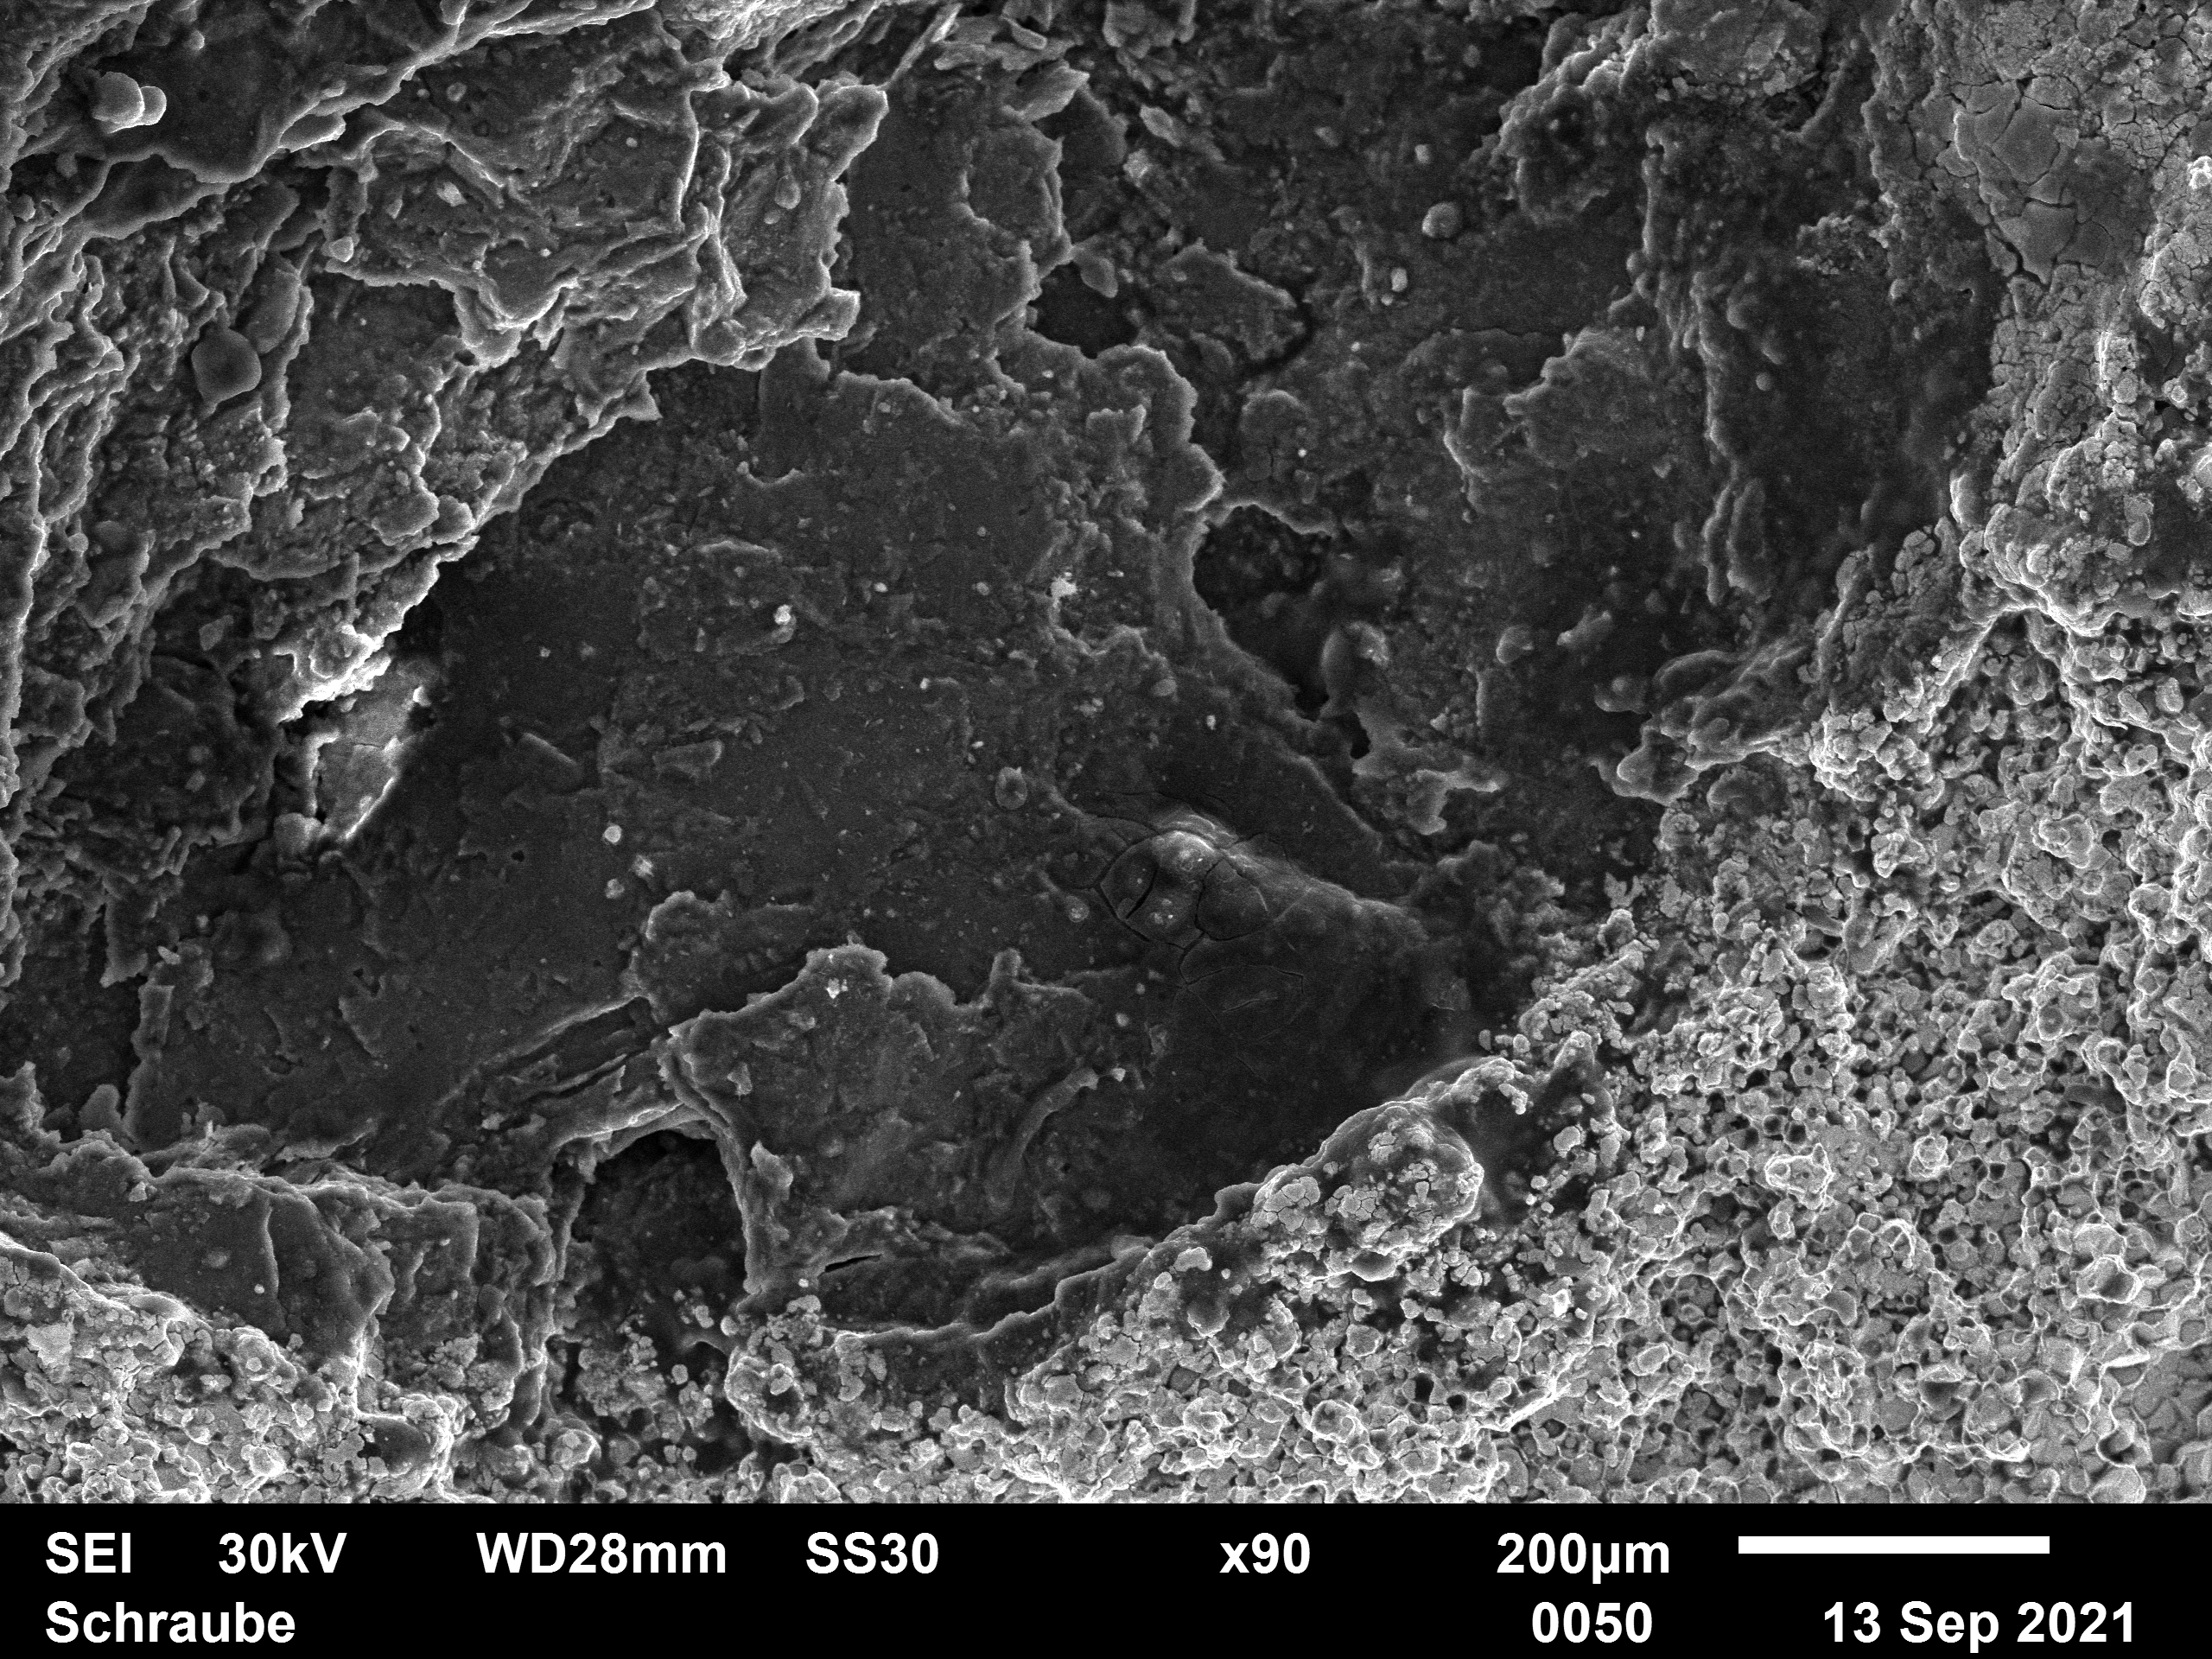
\includegraphics[width=\textwidth]{Auswertung/D/0050.png}
        \caption{SEI}
    \end{subfigure}
    \hfill
    \begin{subfigure}[b]{0.45\textwidth}
        \centering
        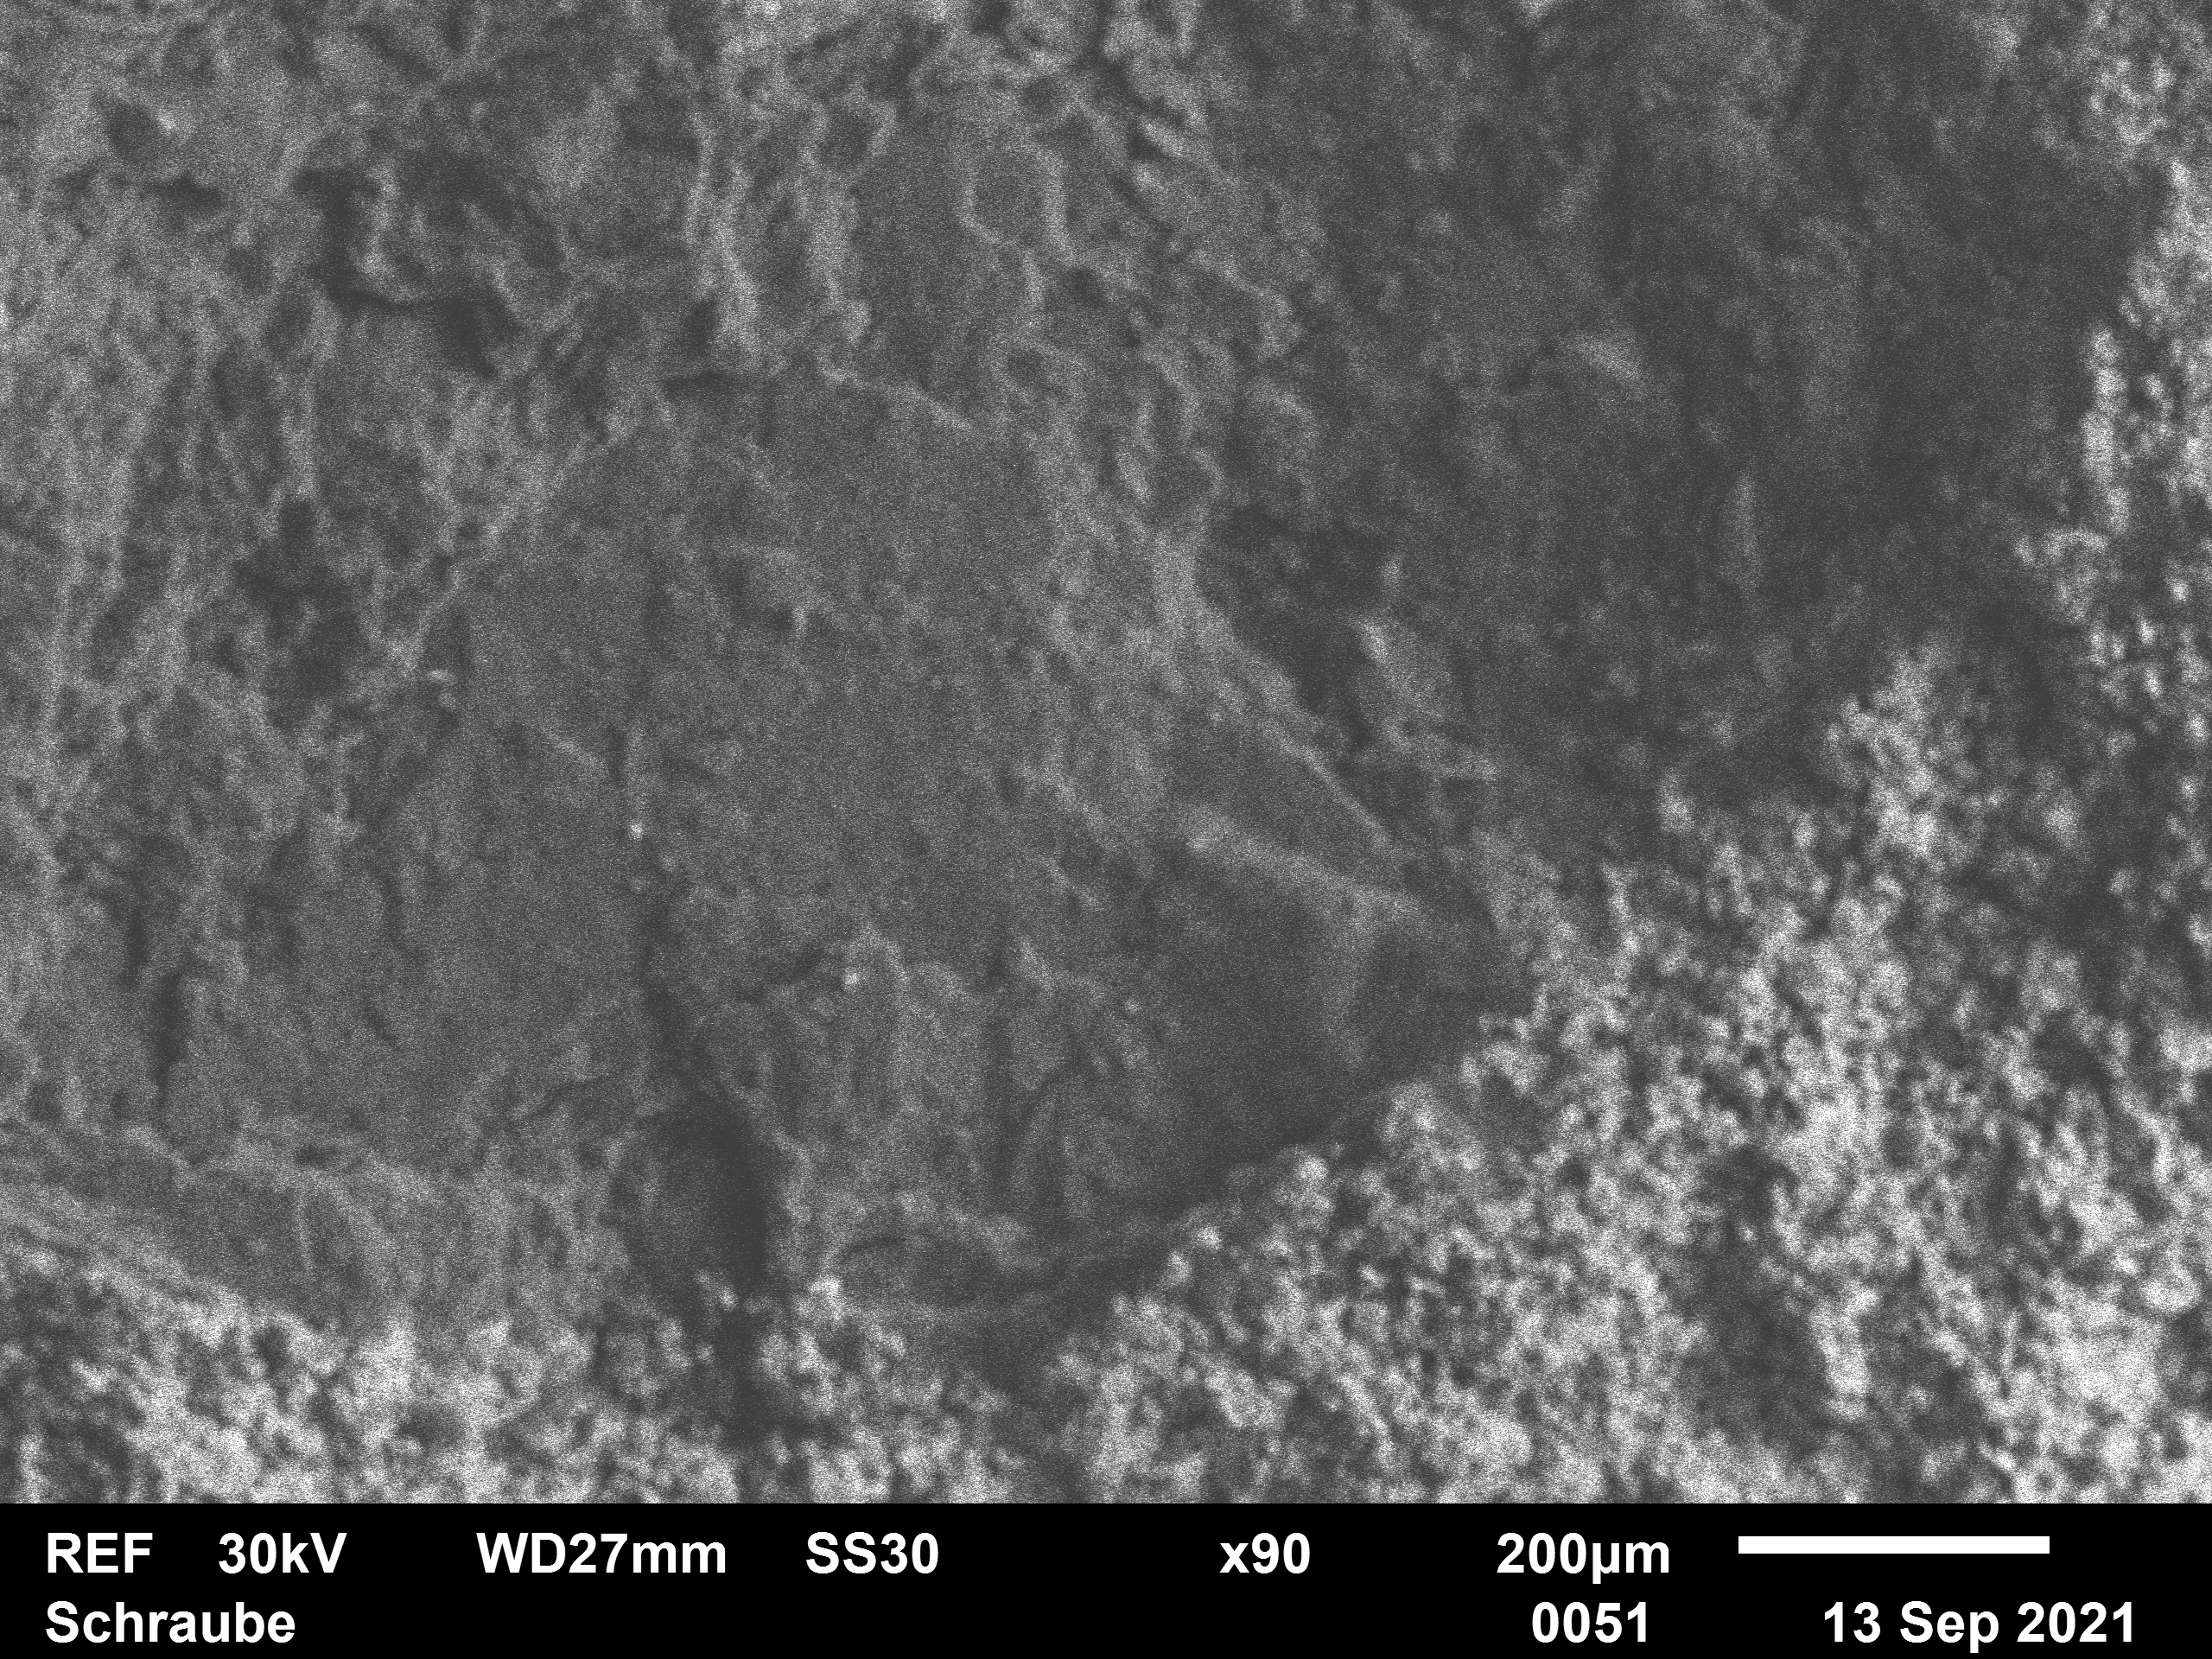
\includegraphics[width=\textwidth]{Auswertung/D/0051.png}
        \caption{REF}
    \end{subfigure}
    \caption{Nahaufnahme der Kante des dunklen Flecks}
\end{figure}

Aus diesen Aufnahmen geht hervor, dass der dunkle Fleck mit einer Vertiefung einhergeht.

\newpage
Nun soll eine EDX Analyse über die Materialzusammensetzung des dunklen Flecks aufschluss geben.
\begin{figure}[h]
    \centering
    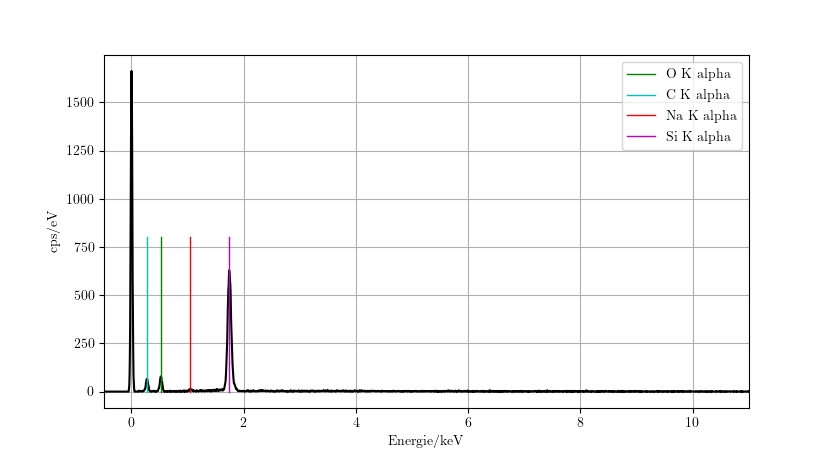
\includegraphics[width=\textwidth]{Auswertung/D/DunkelEDX.png}
    \caption{Röntgenspektrum des dunklen Flecks}
\end{figure}


\begin{table}[h]
    \centering
    \begin{tabular}{c|c|c|c|c|c|c}
        Element & OZ &Serie& unn. C & norm. C &  Atom. C  & Fehler (1 Sigma) \\
         & & & [Gew. \%] & [Gew. \%] & [At. \%] & [Gew. \%] \\
        \hline\hline
        C & 6 & K & 56,69 & 43,02 & 55,43 & 14,77\\
        O & 8 & K & 41,46 & 31,46 & 30,43 & 10,20\\
        Na & 11 & K & 0,89 & 0,67 & 0,45 & 0,16\\
        Si & 14 & K & 32,74 & 24,85 & 13,69 & 1,56
    \end{tabular}
    \caption{Ergebnisse der EDX-Analyse des dunklen Bereichs}
\end{table}

\newpage
Des Weiteren zeigt eine Nahaufnahmeder hellen gegenden, dass sich diese durch eine gewisse Erhabenheit auszeichnen. Außerdem erscheint die Oberfläche in diesem Bereich ebener.
\begin{figure}[h]
    \centering
    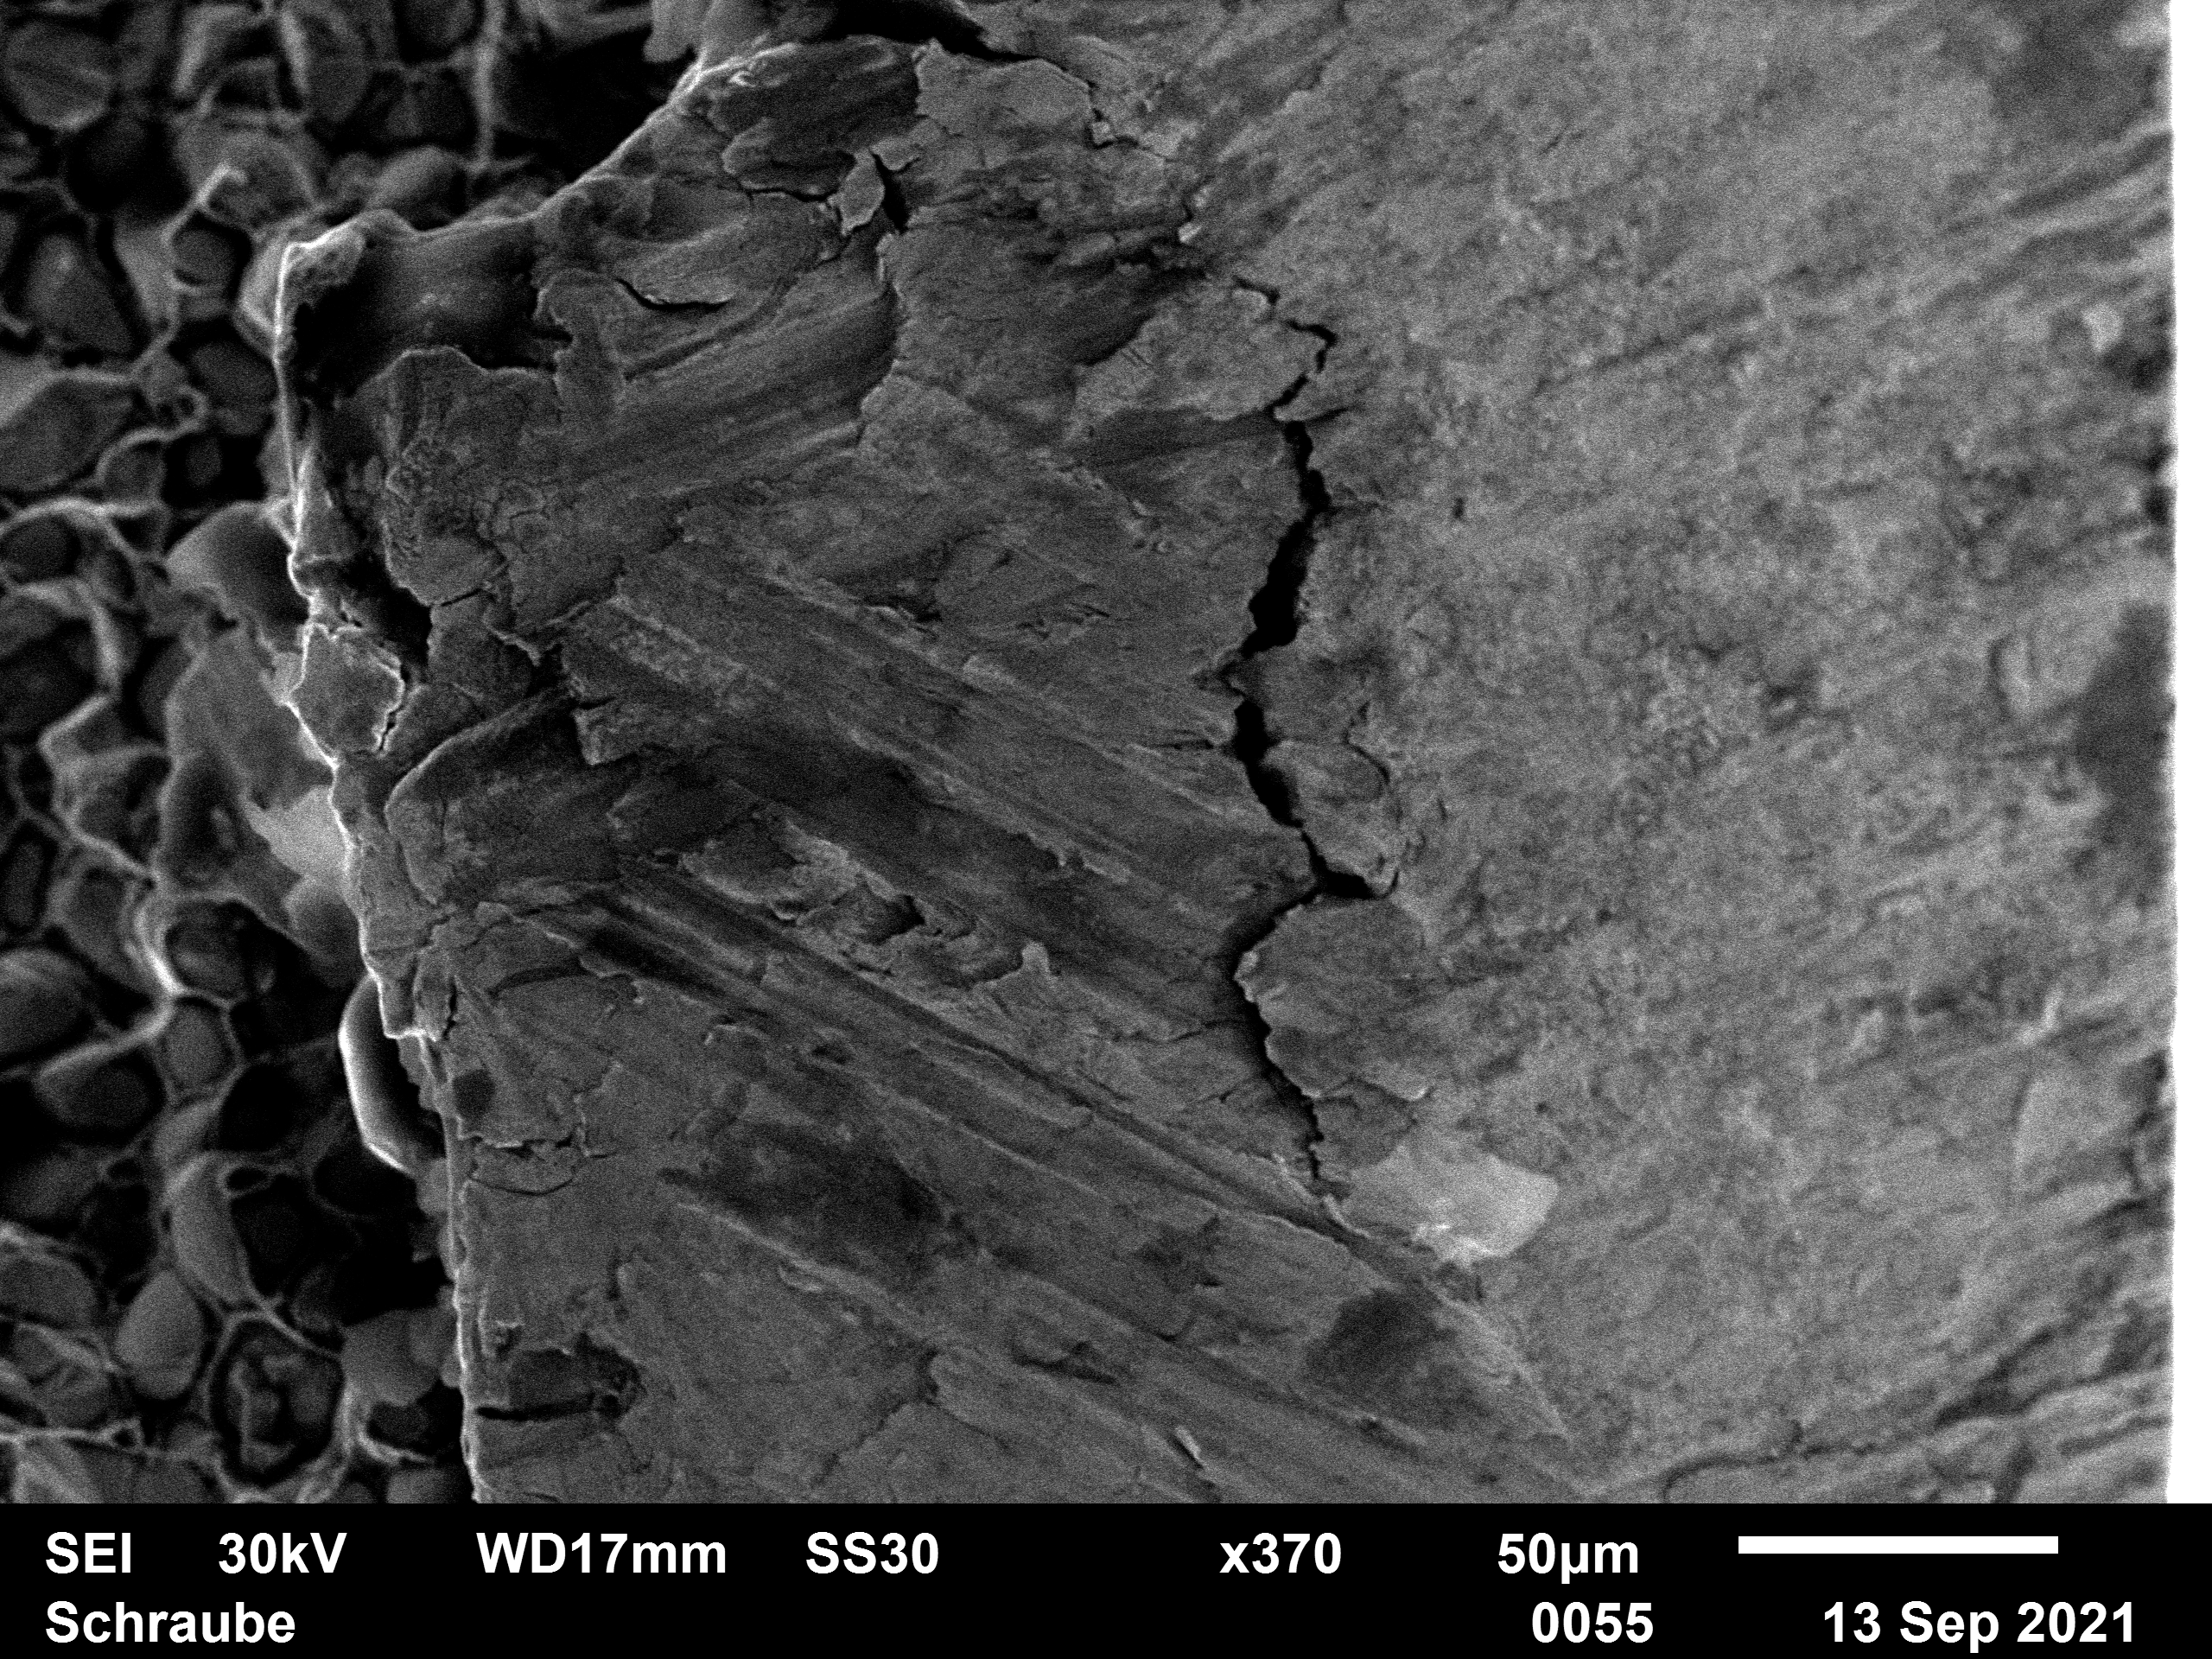
\includegraphics[width=\textwidth]{Auswertung/D/0055.png}
    \caption{Nahaufnahme einer hellen Region}
\end{figure}

\newpage
Über die Zusammensetzung soll wiederum eine EDX Analyse Aufschluss geben.
\begin{figure}[h]
    \centering
    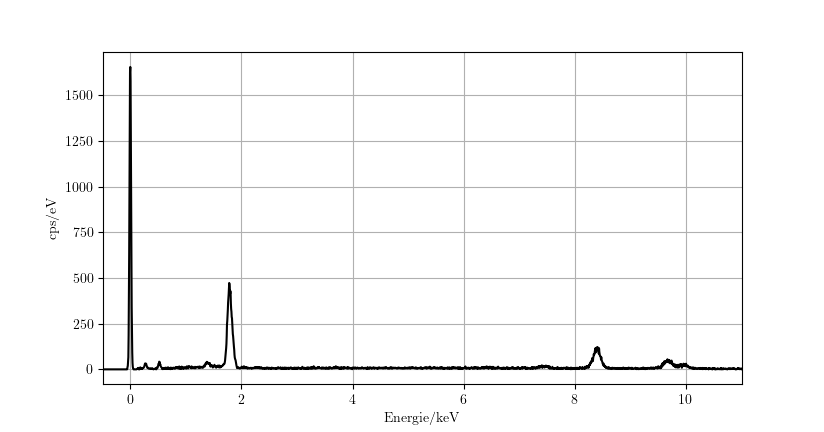
\includegraphics[width=\textwidth]{Auswertung/D/HellEDX.png}
    \caption{Röntgenspektrum der hellen Bereiche}
\end{figure}



\begin{table}[h]
    \centering
    \begin{tabular}{c|c|c|c|c|c|c}
        Element & OZ &Serie& unn. C & norm. C &  Atom. C  & Fehler (1 Sigma) \\
         & & & [Gew. \%] & [Gew. \%] & [At. \%] & [Gew. \%] \\
        \hline\hline
        C & 6 & K & 18,02 & 16,52 & 52,93 & 5,99\\
        O & 8 & K & 14,29 & 13,10 & 31,51 & 4,47\\
        Fe & 26 & K & 0,57 & 0,53 & 0,36 & 0,08\\
        Ni & 28 & K & 1,38 & 1,27 & 0,83 & 0,12\\
        W & 74 & L & 74,81 & 68,59 & 14,36 & 2,09
    \end{tabular}
    \caption{Ergebnisse der EDX-Analyse der hellen Bereiche}
\end{table}

\newpage
Nicht zu vergessen ist das Grundmaterial der Schraube, auch hierbei wird wieder eine EDX Analyse benutzt.
\begin{figure}[h]
    \centering
    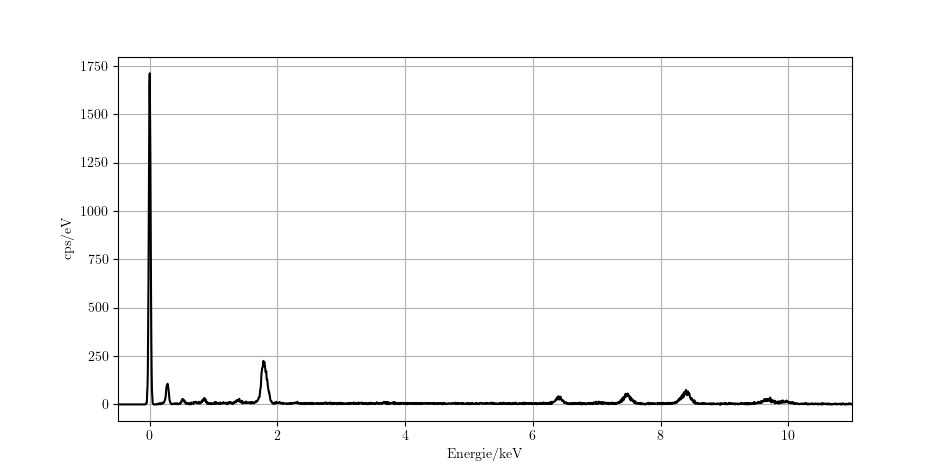
\includegraphics[width=\textwidth]{Auswertung/D/NormalEDX.png}
    \caption{Röntgenspektrum der normalen Bereiche}
\end{figure}


\begin{table}[h]
    \centering
    \begin{tabular}{c|c|c|c|c|c|c}
        Element & OZ &Serie& unn. C & norm. C &  Atom. C  & Fehler (1 Sigma) \\
         & & & [Gew. \%] & [Gew. \%] & [At. \%] & [Gew. \%] \\
        \hline\hline
        C & 6 & K & 42,64 & 43,61 & 78,17 & 9,71\\
        O & 8 & K & 9,86 & 10,08 & 13,57 & 3,42\\
        Fe & 26 & K & 3,94 & 4,03 & 1,55 & 0,20\\
        Ni & 28 & K & 6,88 & 7,04 & 2,58 & 0,28\\
        W & 74 & L & 34,45 & 35,24 & 4,13 & 1,08
    \end{tabular}
    \caption{Ergebnisse der EDX-Analyse der normalen Bereiche}
\end{table}

Unter berücksichtigung der soeben erlangten Erkenntnisse erscheint es als wahrscheinlich, dass der Dunkle Fleck eine Verunreinigung ist, welche bei der Herstellung in die Schmetze gelang. Diese Vermutung wurde am deutlichsten durch die EDX Analyse bestätigt, da dieser Bereich eine völlig andere Materialzusammensetzung besitzt. Die "normalen" und hellen Bereiche setzen sich hingegen aus den gleichen Materialien zusammen. \\

Durch die Verunreinigung (dunkle Anomalie) würde somit die Querschnittsfläche der Legierung an dieser Stelle verkleinert. Dies führte deshalb zu einer verminderung der stabilität, weshalb die Schraube an dieser Stelle gebrochen ist.

\newpage
\section{Chip Wafer}

Im letzten Teil haben wir uns einen Teil eines Chip Wafers vorgenommen. Gut zu erkennen sind die Leiterbahnen. Außerdem konnten wir auch ein Logo finden.

\begin{figure}[h]
    \centering
    
    \begin{subfigure}[b]{0.45\textwidth}
        \centering
        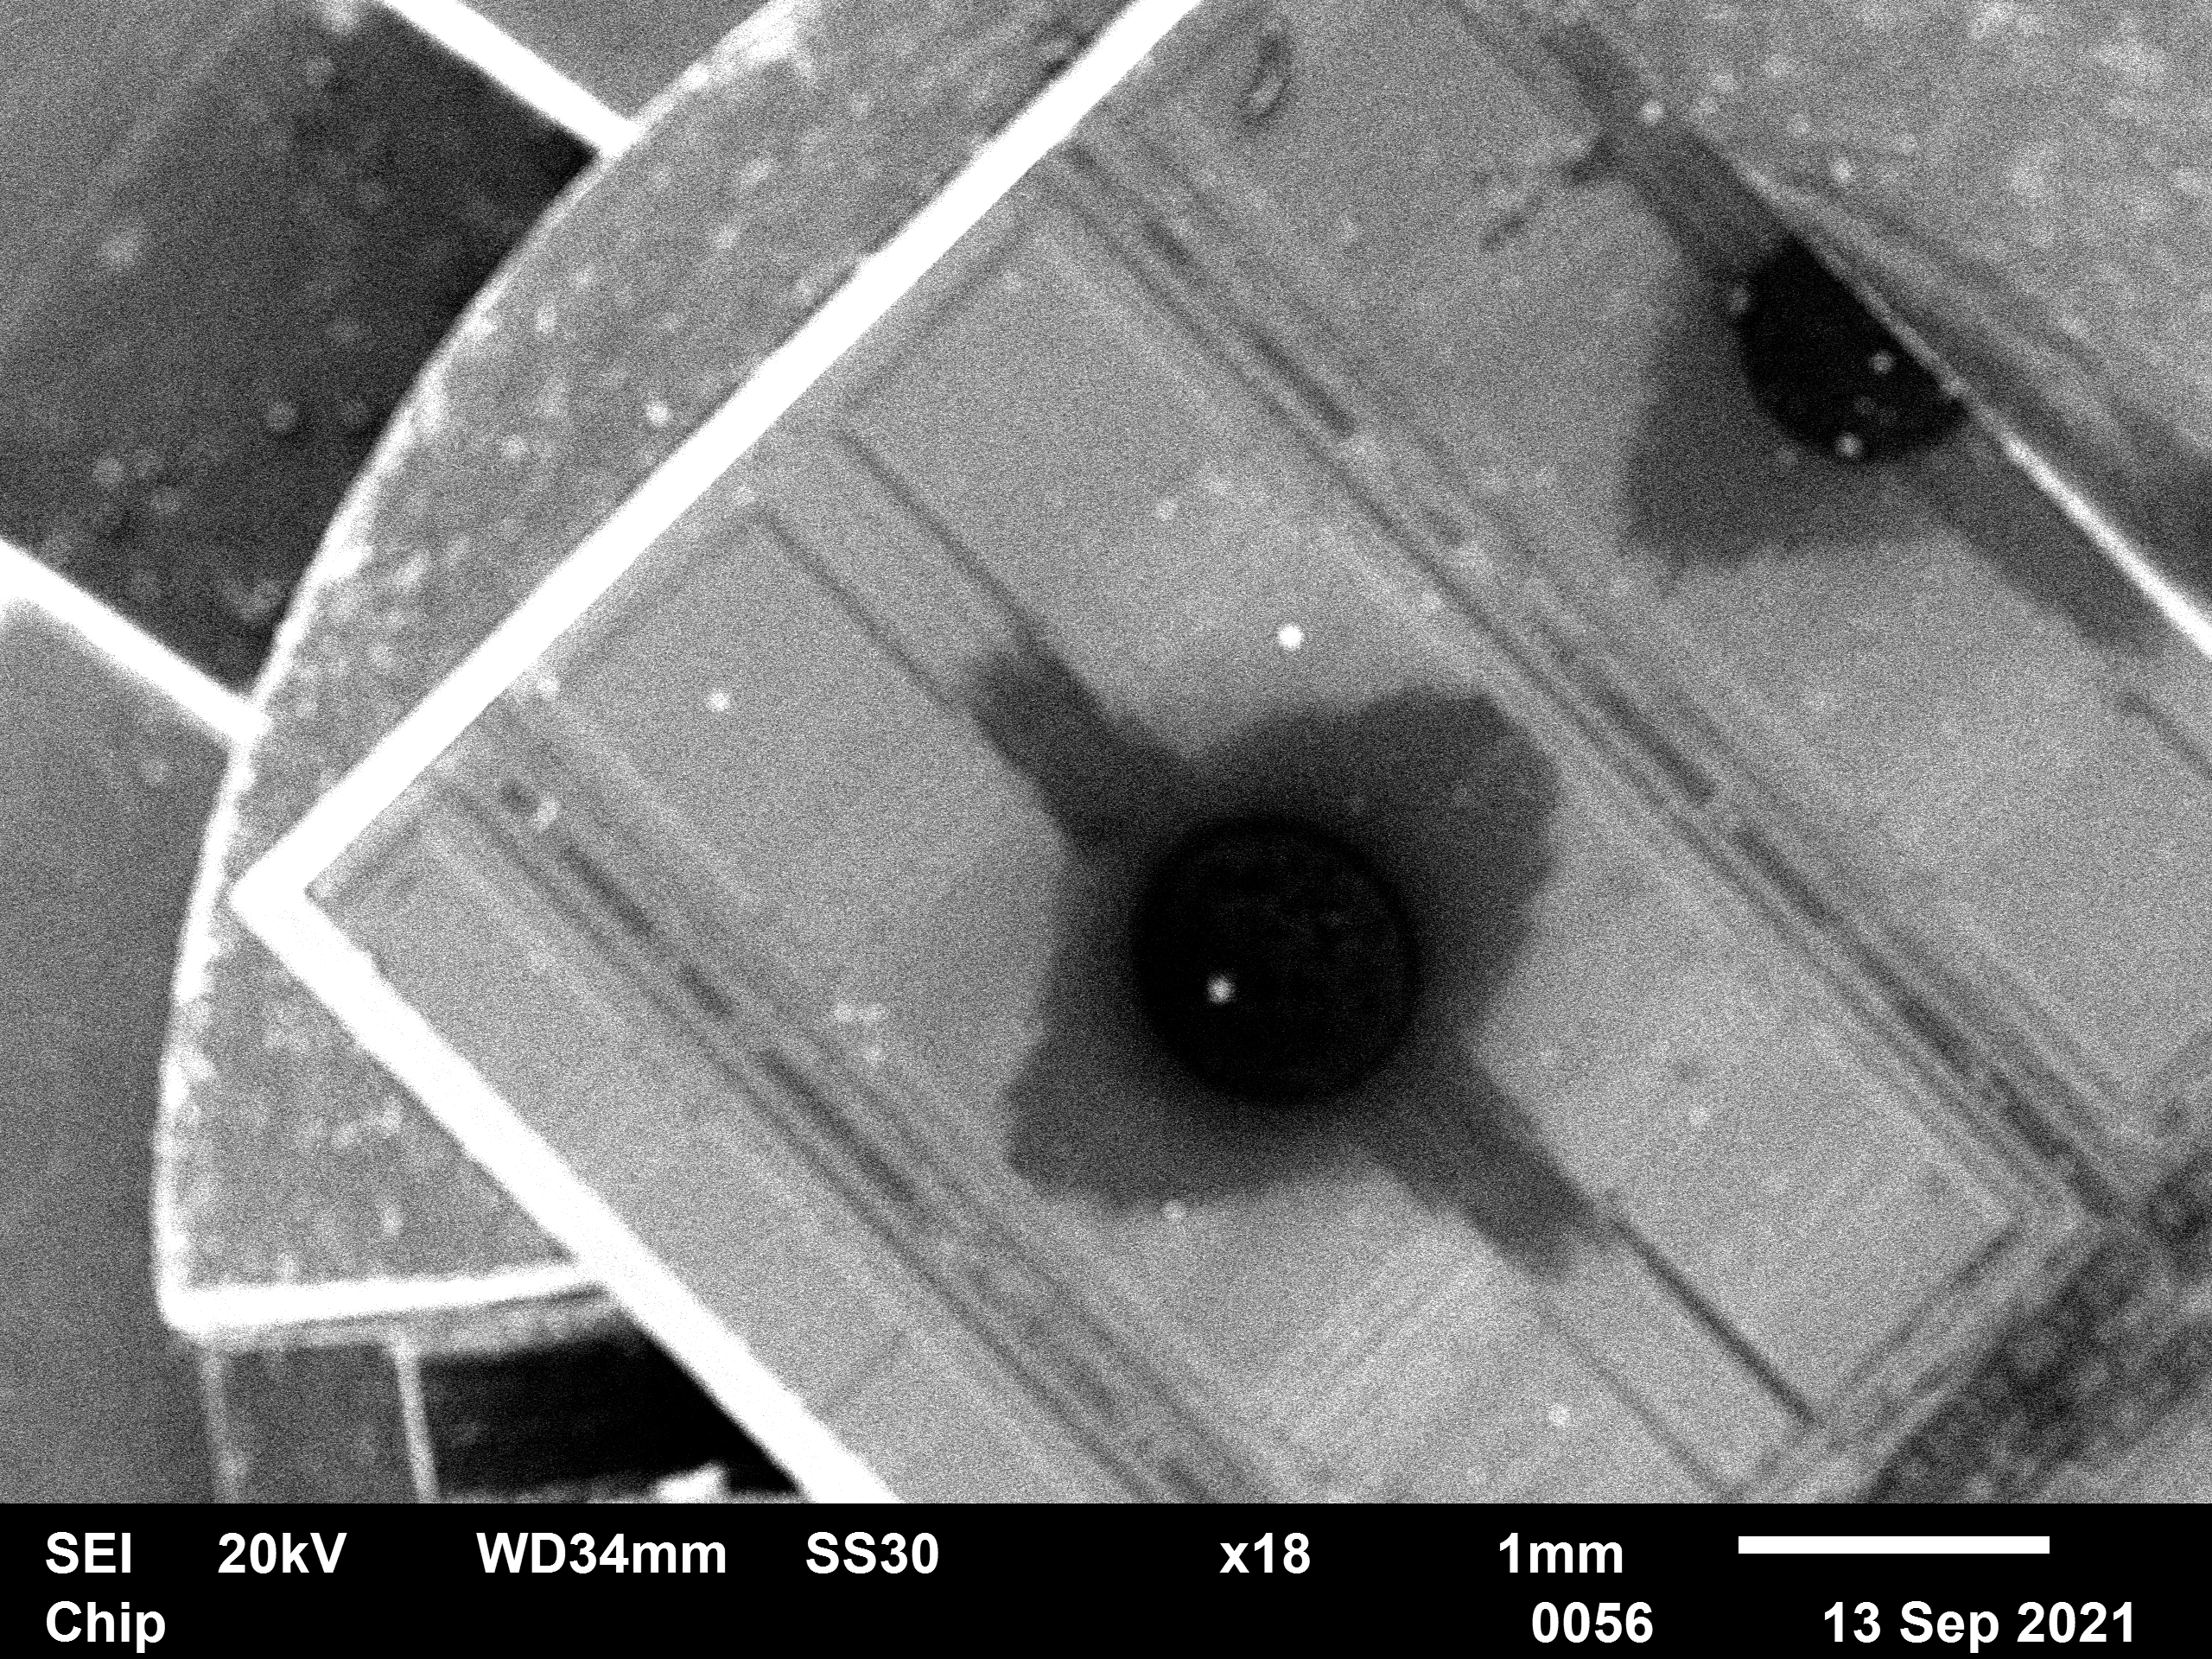
\includegraphics[width=\textwidth]{Auswertung/E/0056.png}
        \caption{Großaufnahme}
    \end{subfigure}
    \hfill
    \begin{subfigure}[b]{0.45\textwidth}
        \centering
        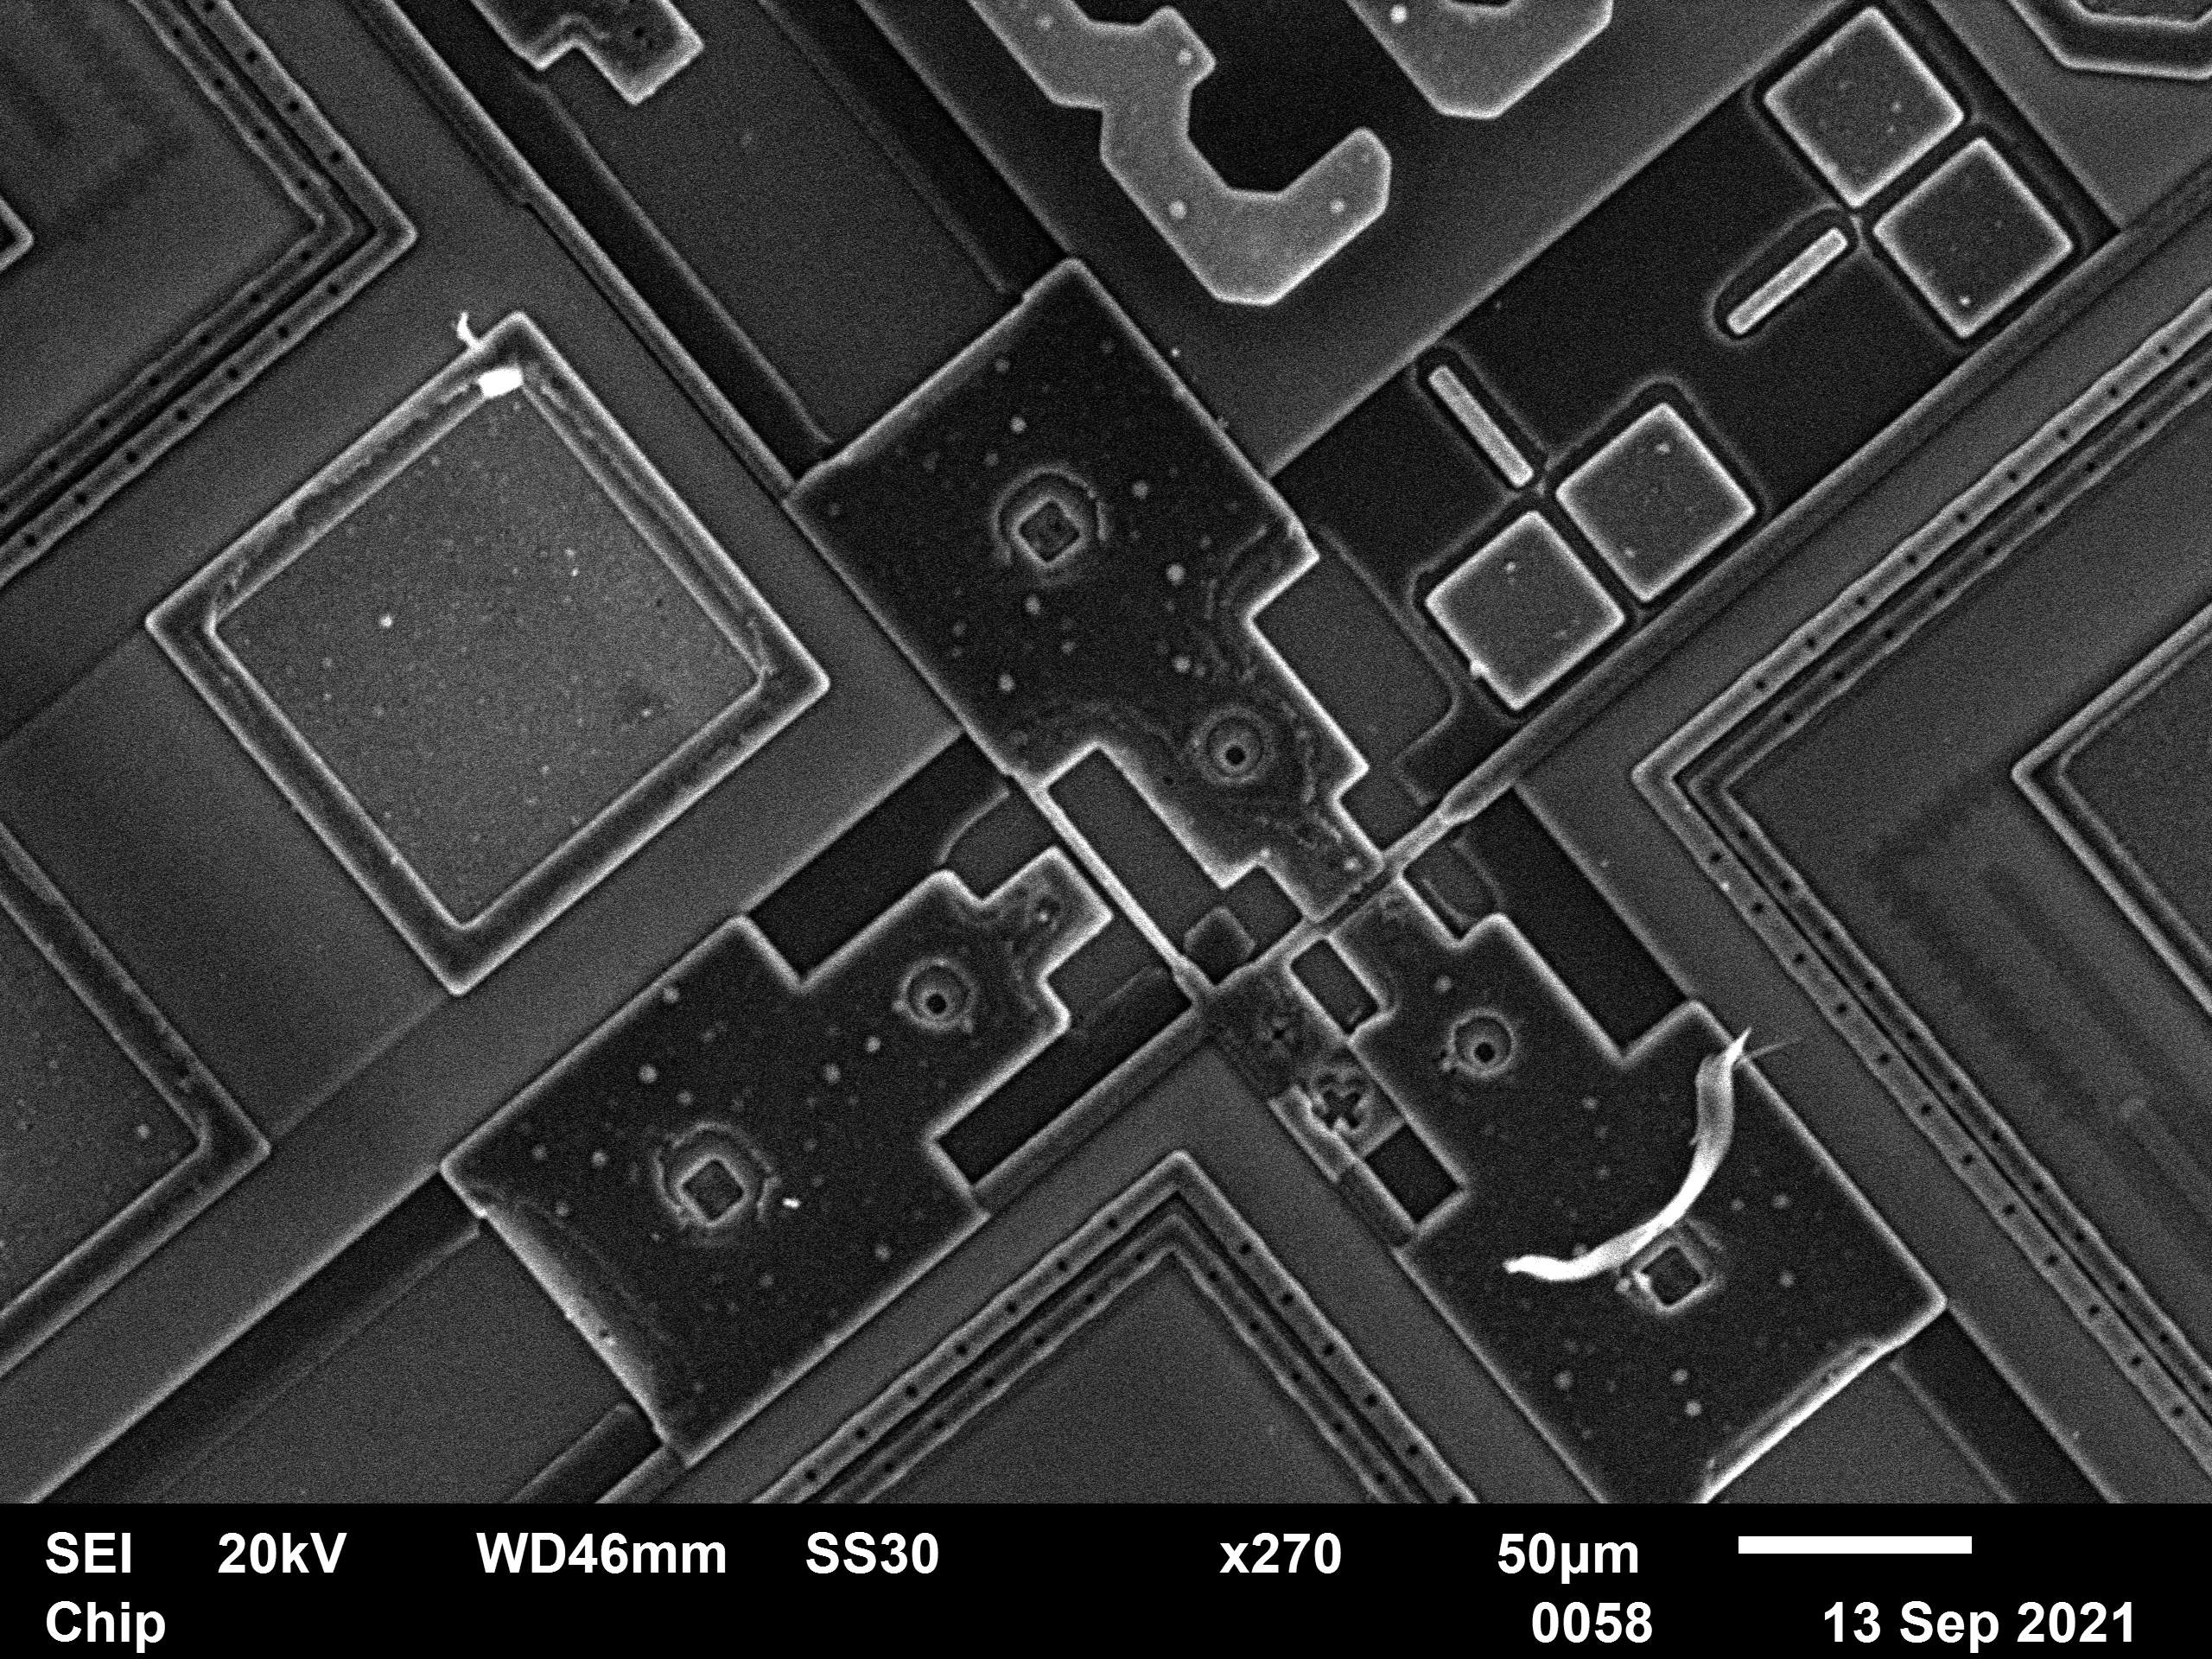
\includegraphics[width=\textwidth]{Auswertung/E/0058.png}
        \caption{Leiterbahnen}
    \end{subfigure}
    \\
    \begin{subfigure}[b]{0.45\textwidth}
        \centering
        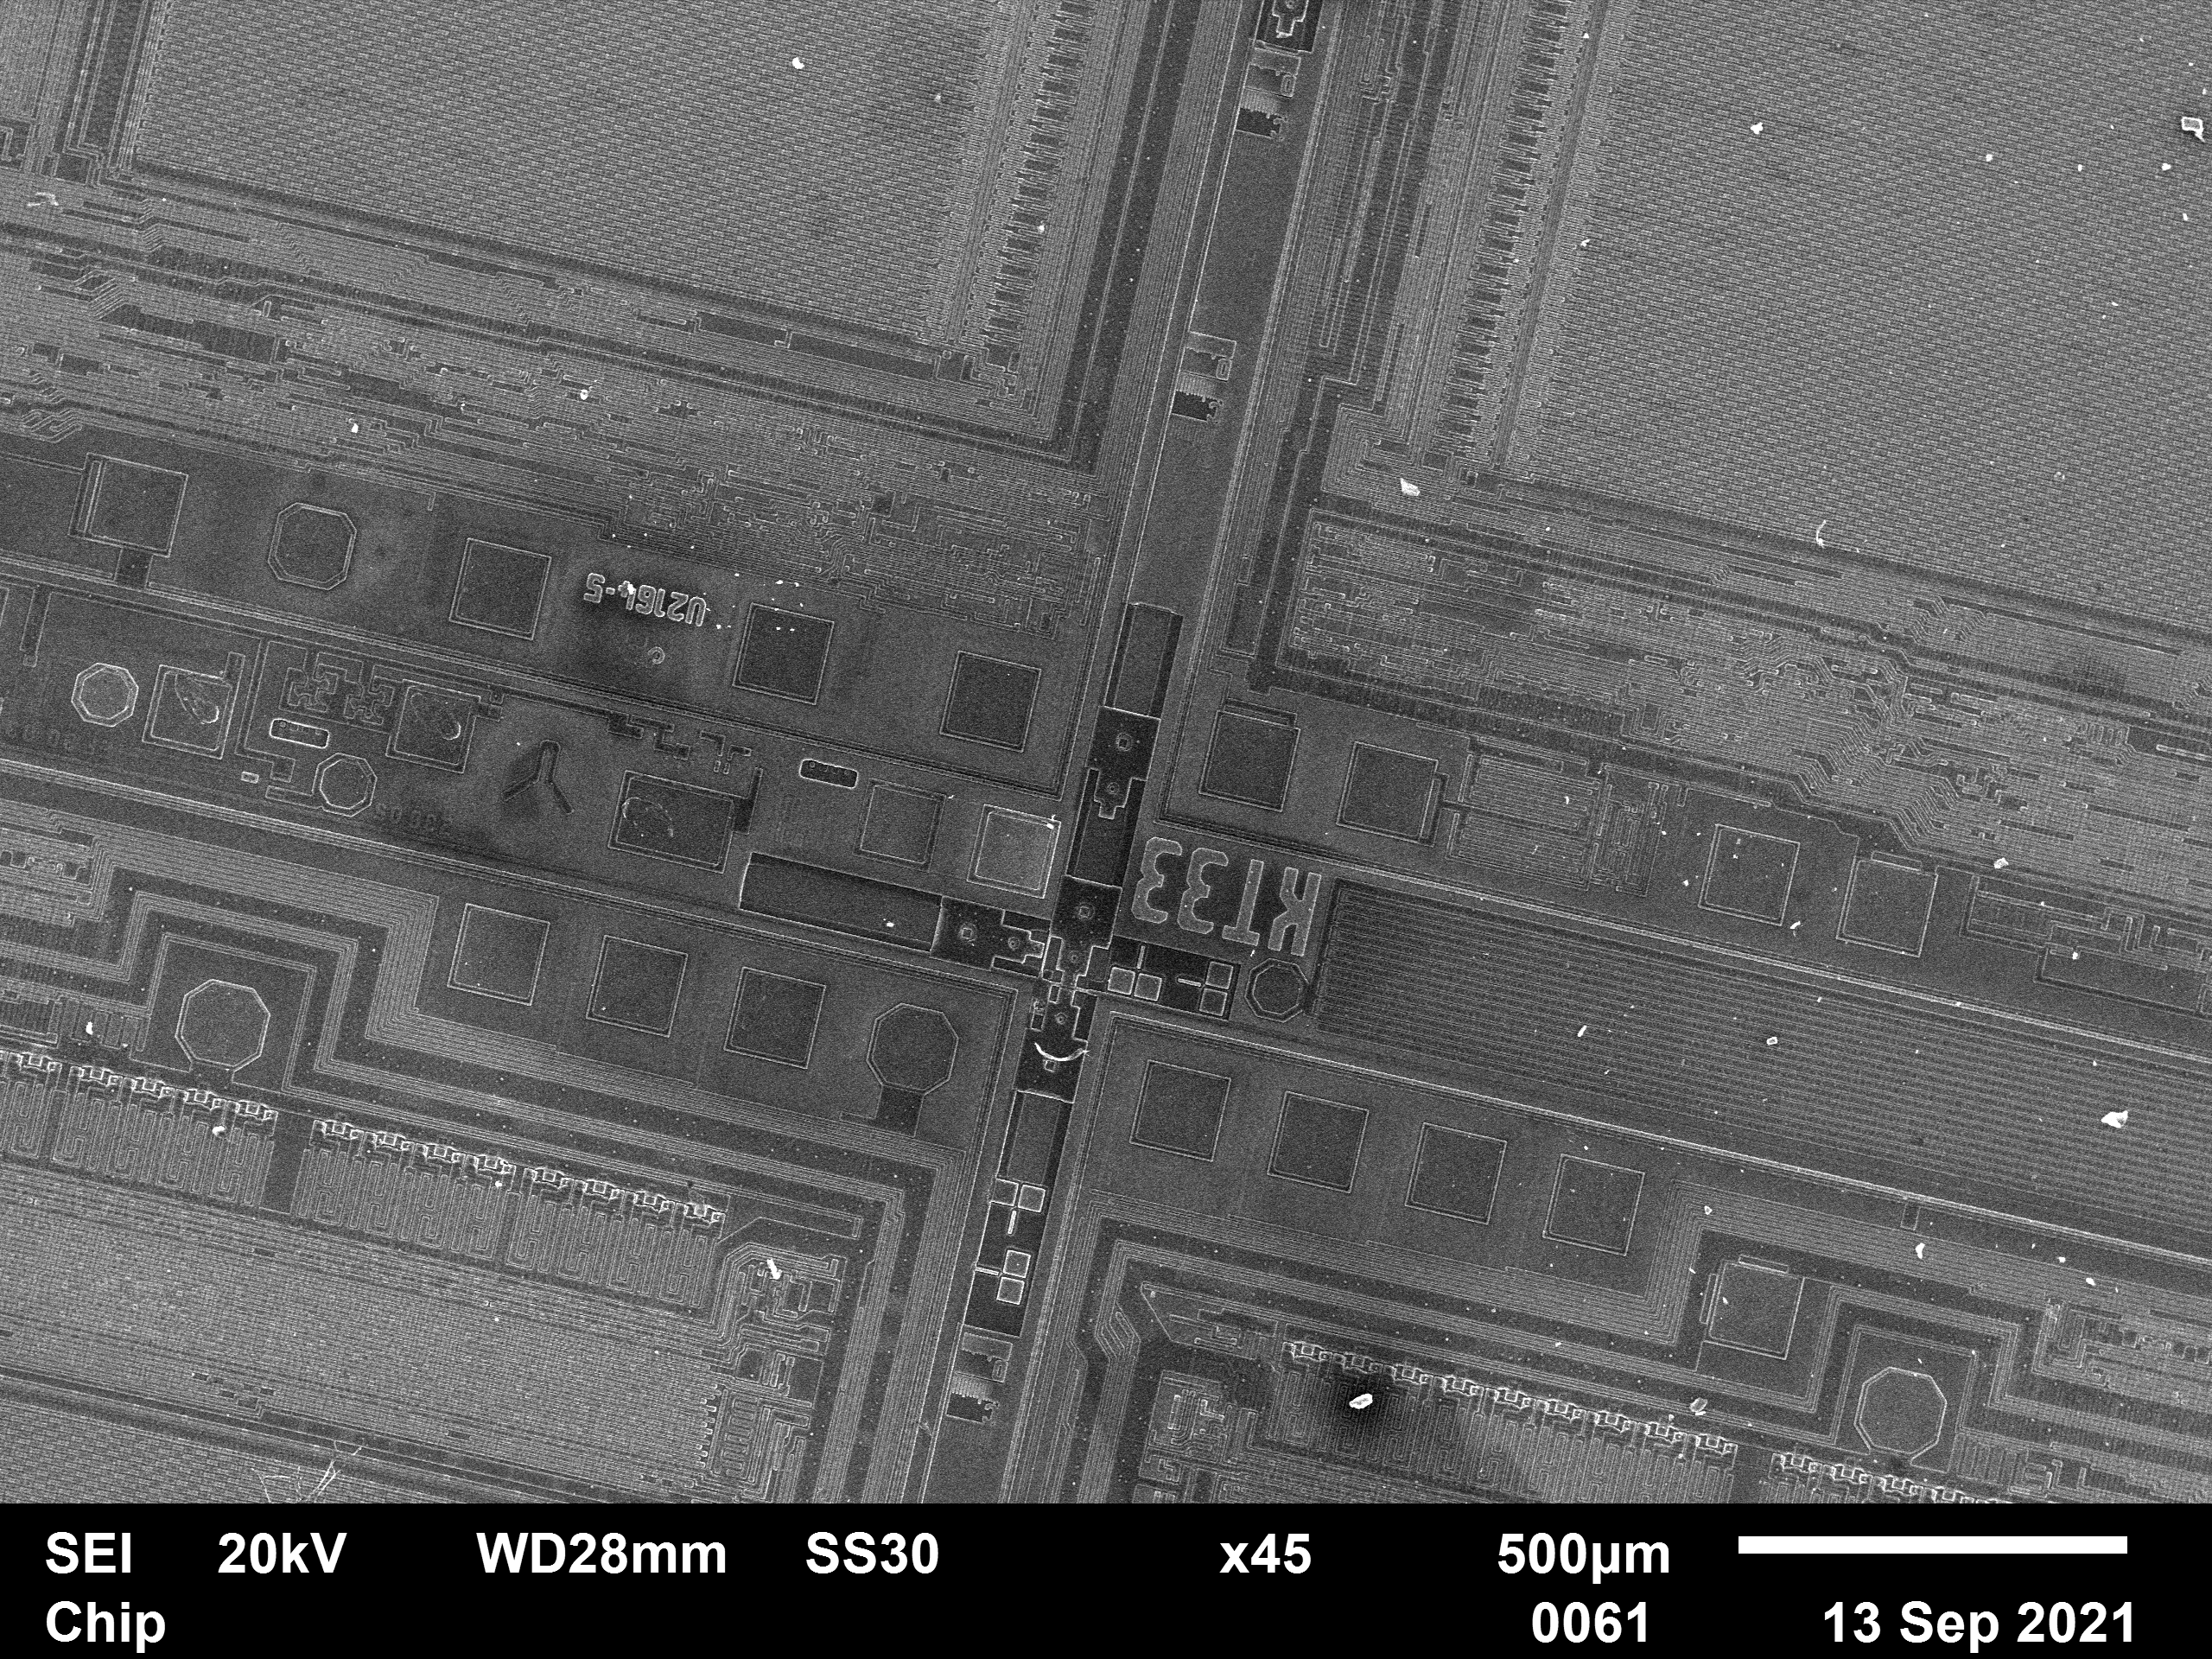
\includegraphics[width=\textwidth]{Auswertung/E/0061.png}
        \caption{Leiterbahnen}
    \end{subfigure}
    \hfill
    \begin{subfigure}[b]{0.45\textwidth}
        \centering
        \includegraphics[width=\textwidth]{Auswertung/E/0063.png}
        \caption{Logo}
    \end{subfigure}
    \caption{Bilder des Wafers}
\end{figure}